\documentclass{llncs}

\usepackage{hyperref}

\usepackage[T1]{fontenc} 
\usepackage[utf8]{inputenc}

% \usepackage{amsmath}
% \usepackage{amssymb}
% \usepackage{graphicx}
\usepackage{comment}
% \usepackage{wrapfig}
%\usepackage{url}
% \usepackage{multirow}
\usepackage{color}
% \usepackage{tabularx}  
% \usepackage{booktabs}
% \usepackage{framed}
\usepackage{boxedminipage}
% \usepackage{tikz}
% \usetikzlibrary{arrows,chains,matrix,positioning,scopes}

% \usepackage{enumitem}

% \usepackage{mathpartir}

\usepackage{listings}

%\newcommand{\code}[1]{\lstinline[language={},basicstyle=\lstinfigurestyle]{#1}}
\newcommand{\smcode}[1]{\lstinline[language={},basicstyle=\lstenumstyle]{#1}}
\newcommand{\lstinlinestyle}{\fontfamily{pcr}\fontsize{9pt}{11pt}\selectfont}
\newcommand{\lstfigurestyle}{\fontfamily{pcr}\fontsize{8pt}{10pt}\selectfont}
\newcommand{\lstenumstyle}{\fontfamily{pcr}\fontsize{9pt}{11pt}\selectfont}

%\lstset{backgroundcolor=\color{lightgray}}
\lstset{rulecolor=\color{lightgray}}
\lstset{basicstyle = \lstfigurestyle}
\lstset{tabsize = 2}
\lstset{numberbychapter=false}
\lstset{frame = single, framerule = 0.05pt}
\lstset{numbers = none, numberstyle = \scriptsize\sffamily}%\textcolor{black}}
\lstset{aboveskip=1.5\smallskipamount, belowskip=\smallskipamount}
\lstset{framexbottommargin=0pt}
\lstset{captionpos = t}
\lstset{escapeinside={/+}{+/}}
\lstset{moredelim=*[is][\underbar]{_}{_}}
\lstset{moredelim=[is][basicstyle]{`}{`}} % to escape non-keyword words
\lstset{showstringspaces=false}

\usepackage{atbegshi,ifthen,tikz}

% change this to customize the appearance of the highlight
\tikzstyle{highlighter} = [
  lightgray,
  line width = \baselineskip,
]

% implementation of the core highlighting logic; do not change!
\newcounter{highlight}[page]
\newcommand{\tikzhighlightanchor}[1]{\ensuremath{\vcenter{\hbox{\tikz[remember picture, overlay]{\coordinate (#1 highlight \arabic{highlight});}}}}}
\newcommand{\bh}[0]{\stepcounter{highlight}\tikzhighlightanchor{begin}}
\newcommand{\eh}[0]{\tikzhighlightanchor{end}}
\AtBeginShipout{\AtBeginShipoutUpperLeft{\ifthenelse{\value{highlight} > 0}{\tikz[remember picture, overlay]{\foreach \stroke in {1,...,\arabic{highlight}} \draw[highlighter] (begin highlight \stroke) -- (end highlight \stroke);}}{}}}

\newcommand{\langname}[1]{#1}

\lstdefinelanguage{SDF} {
	morekeywords={context, free, syntax, start, symbols, lexical, module, imports, exports, avoid, recover, cons, bracket, reject, templates, priorities, left},
	otherkeywords={},
	morecomment=[l]{\%\%},
	sensitive=true,
	mathescape=true
}

\newcommand{\sdfcode}[1]{\lstinline[language=SDF,basicstyle=\lstinlinestyle,breaklines=false]{#1}}
\newcommand{\sdfcodebl}[1]{\lstinline[language=SDF,basicstyle=\lstinlinestyle,breaklines=true]{#1}}
\newcommand{\SDF}{\langname{SDF}}

\lstdefinelanguage{SPT} {
	morekeywords={module, test, parse, succeeds, start, symbol, language},
	otherkeywords={[,]},
	morecomment=[l]{\%\%},
	sensitive=true,
	mathescape=true
}

\newcommand{\sptcode}[1]{\lstinline[language=SDF,basicstyle=\lstinlinestyle,breaklines=false]{#1}}
\newcommand{\sptcodebl}[1]{\lstinline[language=SDF,basicstyle=\lstinlinestyle,breaklines=true]{#1}}
\newcommand{\SPT}{\langname{SPT}}

\lstdefinelanguage{Stratego}{
	morekeywords=[1]{all, bagof, constructors, end, extend, fail, id, imports, in,
	let, module, not, one, overlays, override, prim, rec, rules, script, signature,
	some, sorts, rules, strategies, stratego, test, thread, where, with, if, then,
	else, switch, case, otherwise, depends, on}, 
	alsoletter={-}, 
	otherkeywords={<,<+,+>,?.!,*,>,[,$[,|,]}, 
	%morestring=[b]",
	morecomment=[l]{//},
	morecomment=[n]{(*}{*)},
	morecomment=[n]{/*}{*/},
	literate=
		%{|[}{{\texttt{|$\!\!$[}}}2%
		%{]|}{{\texttt{]$\!\!$|}}}2%
		{->}{$\rightarrow$~}2%
		{=>}{$\Rightarrow$~}2,
	sensitive=true,
	mathescape=false,
	keepspaces=true
}[keywords,comments,strings]

\newcommand{\strcode}[1]{\lstinline[language=Stratego,basicstyle=\lstinlinestyle,breaklines=false]{#1}}
\newcommand{\strcodebl}[1]{\lstinline[language=Stratego,basicstyle=\lstinlinestyle,breaklines=true]{#1}}
\newcommand{\Stratego}{\langname{Stratego}}

\lstdefinelanguage{NaBL} {
  morekeywords={module, namespaces, properties, binding, rules, implicitly, defines, unique, of, in, current, subsequent, scope, scopes, refers, to, enclosing, best, conformant, imports, imported, from, as, into, where, has, otherwise, and, or, by, minimal, distance, filters, disambiguates, else, with, error, surrounding},
  otherkeywords={non-unique,non-transitively},
  morekeywords=[2]{}, %% Namespaces
  morekeywords=[3]{}, %% Properties
  morestring=[b]"
	morecomment=[l]{//},
	morecomment=[n]{/*}{*/},
  literate={...}{$\ldots$}2,
  sensitive=true,
  mathescape=false
}

\newcommand{\nablcode}[1]{\lstinline[language=NaBL,basicstyle=\lstinlinestyle,breaklines=false]{#1}}
\newcommand{\nablcodebl}[1]{\lstinline[language=NaBL,basicstyle=\lstinlinestyle,breaklines=true]{#1}}
\newcommand{\NaBL}{\langname{NaBL}}

\lstdefinelanguage{TS} {
	morekeywords={module, imports,type, rules, definition, of, where, has, else, error, on, and, or,function, functions, defines, relations},
  morestring=[b]",
	morecomment=[l]{//},
	morecomment=[n]{/*}{*/},
  sensitive=true,
  mathescape=false
}

\newcommand{\tscode}[1]{\lstinline[language=TS,basicstyle=\lstinlinestyle,breaklines=false]{#1}}
\newcommand{\tscodebl}[1]{\lstinline[language=TS,basicstyle=\lstinlinestyle,breaklines=true]{#1}}
\newcommand{\TS}{\langname{TS}}

\newcommand{\javacode}[1]{\lstinline[language=Java,basicstyle=\lstinlinestyle,breaklines=false]{#1}}
\newcommand{\javacodebl}[1]{\lstinline[language=Java,basicstyle=\lstinlinestyle,breaklines=true]{#1}}
\newcommand{\Java}{\langname{Java}}
\lstdefinelanguage{DynSem} {
  morekeywords={
    module, imports,
    signature, sorts, constructors, native,
    rules, 
    value, 
    where},
  literate={!=}{$\not\equiv$}1{==}{$\equiv$}1{=>}{$\Rightarrow$}1{->}{$\rightarrow$}1{-->}{$\rightarrow$}1{|-}{$\vdash$}1{|-->}{$\mapsto$}1,
  comment=[l]{\/\/},
  mathescape=true,
  sensitive=true
}

\newcommand{\dynsemcode}[1]{\lstinline[language=DynSem,basicstyle=\lstinlinestyle]{#1}}
\newcommand{\DynSem}{\langname{DynSem}}

\newenvironment{dynsemfragment}{\begin{lstlisting}[language=DynSem]}{
\end{lstlisting}}
\lstdefinelanguage{ATerm} {
  morekeywords={},
  morekeywords=[2]{Variable},
  otherkeywords={non-unique,[,]}, % {+,*,?}, % ,-,>
  literate={...}{$\ldots$}2,
  comment=[l]{\%\%},
  mathescape=true,
  sensitive=true
}

\newcommand{\atermcode}[1]{\lstinline[language=ATerm,basicstyle=\lstinlinestyle]{#1}}

% lstlisting coq style (inspired from a file of Assia Mahboubi)
%
\lstdefinelanguage{Coq}{ 
%
% Anything betweeen $ becomes LaTeX math mode
mathescape=true,
%
% Comments may or not include Latex commands
texcl=false, 
%
% Vernacular commands
morekeywords=[1]{Section, Module, End, Require, Import, Export,
  Variable, Variables, Parameter, Parameters, Axiom, Hypothesis,
  Hypotheses, Notation, Local, Tactic, Reserved, Scope, Open, Close,
  Bind, Delimit, Definition, Let, Ltac, Fixpoint, CoFixpoint, Add,
  Morphism, Relation, Implicit, Arguments, Unset, Contextual,
  Strict, Prenex, Implicits, Inductive, CoInductive, Record,
  Structure, Canonical, Coercion, Context, Class, Global, Instance,
  Program, Infix, Theorem, Lemma, Corollary, Proposition, Fact,
  Remark, Example, Proof, Goal, Save, Qed, Defined, Hint, Resolve,
  Rewrite, View, Search, Show, Print, Printing, All, Eval, Check,
  Projections, inside, outside, Def},
%
% Gallina
morekeywords=[2]{forall, exists, exists2, fun, fix, cofix, struct,
  match, with, end, as, in, return, let, if, is, then, else, for, of,
  nosimpl, when},
%
% Sorts
morekeywords=[3]{Type, Prop, Set, true, false, option},
%
% Various tactics, some are std Coq subsumed by ssr, for the manual purpose
morekeywords=[4]{pose, set, move, case, elim, apply, clear, hnf,
  intro, intros, generalize, rename, pattern, after, destruct,
  induction, using, refine, inversion, injection, rewrite, congr,
  unlock, compute, ring, field, fourier, replace, fold, unfold,
  change, cutrewrite, simpl, have, suff, wlog, suffices, without,
  loss, nat_norm, assert, cut, trivial, revert, bool_congr, nat_congr,
  symmetry, transitivity, auto, split, left, right, autorewrite},
%
% Terminators
morekeywords=[5]{by, done, exact, reflexivity, tauto, romega, omega,
  assumption, solve, contradiction, discriminate},
%
% Control
morekeywords=[6]{do, last, first, try, idtac, repeat},
%
% Comments delimiters, we do turn this off for the manual
morecomment=[s]{(*}{*)},
%
% Spaces are not displayed as a special character
showstringspaces=false,
%
% String delimiters
morestring=[b]",
morestring=[d]�?,
%
% Size of tabulations
tabsize=3,
%
% Enables ASCII chars 128 to 255
extendedchars=false,
%
% Case sensitivity
sensitive=true,
%
% Automatic breaking of long lines
breaklines=false,
%
% Default style fors listings
%basicstyle=\small,
%
% Position of captions is bottom
captionpos=b,
%
% flexible columns
columns=[l]flexible,
%
% Style for (listings') identifiers
identifierstyle={\color{black}},
% Style for declaration keywords
keywordstyle=[1]{\color{eclipse-keywords}},
% Style for gallina keywords
keywordstyle=[2]{\color{eclipse-keywords}},
% Style for sorts keywords
keywordstyle=[3]{\color{eclipse-keywords}},
% Style for tactics keywords
keywordstyle=[4]{\color{eclipse-keywords}},
% Style for terminators keywords
keywordstyle=[5]{\color{eclipse-keywords}},
%Style for iterators
%keywordstyle=[6]{\ttfamily\color{dkpink}},
% Style for strings
%stringstyle=\ttfamily,
% Style for comments
commentstyle={\color{eclipse-comments}},
%
%moredelim=**[is][\ttfamily\color{red}]{/&}{&/},
literate=
    {\\forall}{{\color{dkgreen}{$\forall\;$}}}1
    {\\exists}{{$\exists\;$}}1
    {<-}{{$\leftarrow\;$}}1
    {=>}{{$\Rightarrow\;$}}1
    {==}{{\code{==}\;}}1
    {==>}{{\code{==>}\;}}1
%    {:>}{{\code{:>}\;}}1
    {->}{{$\rightarrow\;$}}1
    {<->}{{$\leftrightarrow\;$}}1
    {<==}{{$\leq\;$}}1
    {\#}{{$^\star$}}1 
    {\\o}{{$\circ\;$}}1 
    {\@}{{$\cdot$}}1 
    {\/\\}{{$\wedge\;$}}1
    {\\\/}{{$\vee\;$}}1
    {++}{{\code{++}}}1
    {~}{{\ }}1
    {\@\@}{{$@$}}1
    {\\mapsto}{{$\mapsto\;$}}1
    {\\hline}{{\rule{\linewidth}{0.5pt}}}1
%
}[keywords,comments,strings]

\newcommand{\coqcode}[1]{\lstinline[language=Coq,basicstyle=\lstinlinestyle]{#1}}

\lstdefinelanguage{PCFM} {
	morekeywords={module, import, include, def, fun, let, letrec, letpar, in, fix,
	ifz, then, else}, morestring=[b]",
	morecomment=[l]{//},
	morecomment=[n]{/*}{*/},
  sensitive=true,
  mathescape=true
}


\newcommand{\pcfmcode}[1]{\lstinline[language=PCFM,basicstyle=\lstinlinestyle,breaklines=false]!#1!}
\newcommand{\pcfmcodefig}[1]{\lstinline[language=PCFM,basicstyle=\lstfigurestyle,breaklines=false]!#1!}
\newcommand{\pcfmcodebl}[1]{\lstinline[language=PCFM,basicstyle=\lstinlinestyle,breaklines=true]!#1!}
\newcommand{\PCFM}{\langname{PCFM}}
\newcommand{\pcfmcodemm}[1]{\lstinline[language=PCFM,basicstyle={\fontfamily{pcr}\fontsize{9pt}{11pt}\selectfont},breaklines=true]!#1!}


\lstdefinelanguage{paplj} {
	morekeywords={program, run, class, this, Num, Bool, let, in},
	otherkeywords={},
	morecomment=[l]{\%\%},
	sensitive=true,
	mathescape=true
}

\newcommand{\papljcode}[1]{\lstinline[language=SDF,basicstyle=\lstinlinestyle,breaklines=false]{#1}}
\newcommand{\papljcodebl}[1]{\lstinline[language=SDF,basicstyle=\lstinlinestyle,breaklines=true]{#1}}
\newcommand{\paplj}{\langname{PAPLJ}}


\renewcommand{\ldots}{..}
\renewcommand{\texttt}[1]{\smcode{#1}}



\definecolor{eclipse-keywords}{rgb}{0.55,0,0.337}
\definecolor{eclipse-strings}{rgb}{0.165,0,1}
\definecolor{eclipse-comments}{rgb}{0.247,0.498,0.373}
\definecolor{eclipse-keywords2}{rgb}{0,0.25,0.5}

\definecolor{RoyalBlue}{cmyk}{1,0.50,0,0}


% \newcounter{rqno}
\newcommand{\rqdef}[1]{\refstepcounter{rqno}\emph{RQ\arabic{rqno}}\label{rq:#1}}
\newcommand{\rqref}[1]{\emph{RQ\ref{rq:#1}}}

\newcommand{\sectionlabel}[1]{\label{sec:#1}}
\newcommand{\figurelabel}[1]{\label{fig:#1}}
\newcommand{\listinglabel}[1]{\label{lst:#1}}
\newcommand{\appendixlabel}[1]{\label{apx:#1}}
\newcommand{\tablelabel}[1]{\label{tbl:#1}}

\newcommand{\sectionref}[1]{\ref{sec:#1}}
\newcommand{\figureref}[1]{\ref{fig:#1}}
\newcommand{\listingref}[1]{\ref{lst:#1}}
\newcommand{\appendixref}[1]{\ref{apx:#1}}
\newcommand{\tableref}[1]{\ref{tbl:#1}}

\newcommand{\Section}[1]{Section~\sectionref{#1}}
\newcommand{\Sections}[1]{Sections~#1}
\newcommand{\Figure}[1]{Fig.~\figureref{#1}}
\newcommand{\Figures}[1]{Figures~#1}
\newcommand{\Listing}[1]{Listing~\listingref{#1}}
\newcommand{\Listings}[1]{Listings~#1}
\newcommand{\Appendix}[1]{Appendix~\appendixref{#1}}
\newcommand{\Appendices}[1]{Appendices~#1}
\newcommand{\Table}[1]{Table~\tableref{#1}}
\newcommand{\Tables}[1]{Tables~#1}

%\newtheorem{lemma}{Lemma}
%\newtheorem{thm}{Theorem}
%\newtheorem{def}{Definition}

\newcommand{\mynote}[2]
     %%{\sorrynotesaredisallowedatthispoint}
     {{\bfseries\sffamily\scriptsize#1~{\small$\blacktriangleright$\textsf{\emph{#2}}$\blacktriangleleft$}}}

\newcommand\TODO[1]{\mynote{TODO}{#1}}

\newcommand{\AP}[1]{\mynote{AP}{#1}}
\newcommand{\EV}[1]{\mynote{EV}{#1}}
\newcommand{\PN}[1]{\mynote{PN}{#1}}
\newcommand{\APT}[1]{\mynote{APT}{#1}}
\newcommand{\GW}[1]{\mynote{GW}{#1}}
\newcommand{\cfg}{\ensuremath{G = (N, \Sigma, P, S)}}
\newcommand{\symbols}{\ensuremath{\left(N \cup \Sigma\right)^*}}
\newcommand{\derive}[1]{\ensuremath{\Rightarrow_{#1}}}
\newcommand{\prule}[2]{\ensuremath{\left(#1,#2\right)}}

\newcommand{\kw}[1]{\text{\lmrcodefig{#1}}}
\newcommand{\sep}[1]{\text{\lmrcode{#1}}}
\newcommand{\w}[1]{\ensuremath{\mathit{#1}}}
\newcommand{\te}[1]{\ensuremath{\mathrm{#1}}}

\newcounter{grammarrule}
\newenvironment{grammar}
{\small
\setcounter{grammarrule}{0}
\begin{math}\begin{array}{rrcl}}
{\end{array}\end{math}}

\newcommand{\sdn}[3]{#1 & \w{#2} & = & #3}
\newcommand{\sdnn}[2]{\sdn{}{#1}{#2}}
\newcommand{\sd}[2]{\stepcounter{grammarrule}\sdn{\pno{\arabic{grammarrule}}}{#1}{#2}}
\newcommand{\mc}[2]{ & #1 &  & \mbox{#2}}

\newcommand{\altf}[1]{\ |\ #1}
\newcommand{\altn}[2]{\\ #1 & & | & #2}
\newcommand{\altnn}[1]{\altn{}{#1}}
\newcommand{\alt}{\stepcounter{grammarrule}\altn{\pno{\arabic{grammarrule}}}}
\newcommand{\ks}[1]{\ensuremath{#1^*}}
\newcommand{\opt}[1]{\ensuremath{#1?}}

\lstdefinestyle{black-white}
       {keywordstyle=[2]\textit}
\lstdefinestyle{colours}{%
  keywordstyle={\color{eclipse-keywords}}, %
  keywordstyle=[2]{\color{eclipse-strings}}, %
  keywordstyle=[3]{\color{eclipse-keywords2}}, %
  stringstyle={\color{eclipse-strings}}, %
  commentstyle={\color{eclipse-comments}\textit}, %
}
%\lstset{style=colours}
% 
% Judgements
\newcommand{\firstdec}[1]{\emph{#1}\medskip}
\newcommand{\firstdecj}[2]{\emph{#1}\hfill\framebox{\framebox{#2}}\medskip}
\newcommand{\dec}[1]{\medskip\emph{#1}\medskip}
\newcommand{\decj}[2]{\medskip\emph{#1}\hfill\framebox{\framebox{#2}}\medskip}
\newcommand{\wfj}[2]{\ensuremath{#1\ \vdash #2}}
\newcommand{\wtsj}[4]{\ensuremath{#1\ \vdash #2#3 #4}}
\newcommand{\wtj}[3]{\wtsj{#1}{#2}{\,:\,}{#3}}
\newcommand{\wfji}[3]{\ensuremath{#2\ \vdash_{#1} #3}}
\newcommand{\wtjsi}[5]{\ensuremath{#2\ \vdash_{#1} #3#4 #5}}
\newcommand{\wtji}[4]{\wtsj{#1}{#2}{#3}{\,:\,}{#4}}
\newcommand{\ioj}[3]{\ensuremath{#1\ \vdash #2 \Downarrow #3}}
\newcommand{\iouj}[4]{\ensuremath{#2\ \vdash_{#1} #3 \Downarrow #4}}
\newcommand{\applyj}[3]{\ensuremath{\applyf{#1}{#2} = #3}}
\newcommand{\applyf}[2]{\ensuremath{#1\!\left(#2\right)}}
\newcommand{\domj}[2]{#2 \not\in \applyf{\mathit{dom}}{#1}}

\newcommand{\proj}[2]{\applyf{\pi_{#2}}{#1}}
\newcommand{\fst}[1]{\proj{#1}{1}}
\newcommand{\snd}[1]{\proj{#1}{2}}
% tuple
\newcommand{\tpl}[1]{\ensuremath{\langle\,#1\,\rangle}}

% rule name
\newcommand{\tg}[1]{{[}\ensuremath{\mathsf{#1}}{]}}

% axiom
\newcommand{\ax}[2]{\ensuremath{%
\begin{array}[b]{c}
#2
\end{array}\hfill
\begin{tabular}[c]{r}\vspace{.5em}{\tg{#1}}
\end{tabular}\medskip
}}

% inference rule
\newcommand{\ir}[3]{\ensuremath{%
\begin{array}[b]{c}
#2
\\ \midrule
#3
\end{array}\hfill
\begin{tabular}[b]{r}\vspace{.5em}\tg{#1}
\end{tabular}\bigskip
}}


\newcommand{\infrule}[3]{\ensuremath{%
\hfill\dfrac{
  \displaystyle #2
}{
  \displaystyle #3
}\hspace*{\fill}\makebox[0pt][r]{(\ensuremath{#1})}
}}
\newcommand{\infruleL}[3]{\ensuremath{%
\makebox[0pt][l]{(\ensuremath{#1})}\hfill\dfrac{
  \displaystyle #2
}{
  \displaystyle #3
}\hfill
}}
\newcommand{\infrulenl}[2]{\ensuremath{%
\hfill\dfrac{
  \displaystyle #1
}{
  \displaystyle #2
}\hfill}}


\newcommand{\labeled}[2]{\ensuremath{%
\hfill\ensuremath{\displaystyle #2}\hfill\makebox[0pt][r]{(\ensuremath{#1})}
}}
\newcommand{\labeledL}[2]{\ensuremath{%
\makebox[0pt][r]{(\ensuremath{#1})}\hfill\ensuremath{\displaystyle #2}\hfill
}}

\newcommand{\display}[1]{
\bigskip #1 \bigskip
}

% axiom as inference rule
\newcommand{\axr}[2]{\ir{#1}{}{#2}}

% premises
\newcommand{\psep}{\wedge} % change for implicit conjunctions
\newcommand{\pno}[1]{\ensuremath{\mathsf{(#1)}}}
\newcommand{\sps}[1]{\begin{array}{lll}&#1\end{array}}
\newcommand{\np}{\\\psep&}
\newcommand{\nsps}[2]{\begin{array}{rcll}\!\!\!\!\pno{#1}&&#2\end{array}}
\newcommand{\nnsps}[1]{\begin{array}{ccll}&&#1\end{array}}
\newcommand{\nnp}[1]{\\\!\!\pno{#1}&\psep&}
\newcommand{\nnnp}{\\&\psep&}
\newcommand{\dnp}{\ \ \psep\ \ }

% \newcommand{\prf}[1]{\ensuremath{\begin{array}{crll}&&#1\end{array}}}
% \newcommand{\iffnn}{&\Leftrightarrow\\&&}
% \newcommand{\iffn}[1]{&\Leftrightarrow\\&&&}
% \newcommand{\andnn}{\\&\wedge&}
% \newcommand{\andn}[1]{\\(#1) &\wedge&}
% \newcommand{\nmb}[1]{\\(#1) &&}

\newcommand{\prf}[1]{\begin{displaymath}\begin{array}{ccrll}&&&#1\end{array}\end{displaymath}}
\newcommand{\lbrk}{\\&&&\qquad}
\newcommand{\iffnn}{\\\Leftrightarrow&&&}
\newcommand{\iffn}[1]{\\\Leftrightarrow&(#1)&&}
\newcommand{\ifnn}{\\\Rightarrow&&&}
\newcommand{\ifn}[1]{\\\Rightarrow&(#1)&&}
\newcommand{\andnn}{\\&&\wedge&}
\newcommand{\andn}[1]{\\&(#1) &\wedge&}
\newcommand{\nmb}[1]{\\&(#1) &&}
\newcommand{\vds}{\\\vdots&&&}
\newcommand{\avds}{\\&&\vdots&}

% Commands used in nabl-semantics
% Shortcut for the semantic interpretation
\newcommand{\semop}[1]{[\![ #1 ]\!]}
\newcommand{\sem}[2]{\semop{#1}(#2)}
% PCFM code for math mode
\newcommand{\semcode}[1]{\text{\pcfmcodefig{#1}}}
% Formula for regular interpretation translation
\newcommand{\semf}[4]{
 $\semop{#1}(#2) = #3$\\
\smallskip
\qquad$\text{\textsf{where}} \ #4 $
}
\newcommand{\semfs}[4]{
$\sems{#1}{#2} = #3$\\
\smallskip
\qquad$\text{\textsf{where}} \ #4 $
}
\newcommand{\semfp}[5]{
$\semp{#1}{#2}{#3} = #4$\\
\smallskip
\qquad$\text{\textsf{where}} \ #5 $
}

\newcommand{\semfline}[4]{
 $\semop{#1}(#2) = #3 \quad\text{\textsf{where}} \ #4 $
}

\newcommand{\semp}[3]{\semop{#1}^p(#2,#3)}
\newcommand{\sems}[2]{\semop{#1}^s(#2)}

\newcommand{\sappend}{\ \text{+=}\ }
\newcommand{\sdefine}{\ \text{:=}\ }

%\newcommand{\sig}{\ensuremath{\Sigma}}
\newcommand{\sort}{\ensuremath{\sigma}}%{\mathcal{S}}
\newcommand{\sorts}{\ks{\sort}}
\newcommand{\cons}{\w{cn}}%{\mathcal{C}}
\newcommand{\term}{\ensuremath{t}}%{\mathcal{T}}
\newcommand{\trms}{\ks{\term}}
\newcommand{\trmsi}{\cns{\term_0}{\cns{\ldots}{\term_n}}}

\newcommand{\pos}{\w{p}}
%\newcommand{\Pos}{\w{P}}

\newcommand{\idsort}{\kw{id}}
\newcommand{\id}{\w{x}}
\newcommand{\idp}{\iota}
\newcommand{\Idp}{\w{I}}
\newcommand{\Defs}{\mathcal{D}}

\newcommand{\scope}{\w{s}}
\newcommand{\Scopes}{\w{S}}
\newcommand{\pscope}{\scope_\w{p}}
\newcommand{\PosScope}{\w{P}}
\newcommand{\DefScopes}{\Scopes_\w{def}}
\newcommand{\Imports}{\Idp_\w{imp}}

\newcommand{\brule}{\w{r}}
\newcommand{\brules}{\w{R}}

\newcommand{\env}{\ensuremath{E}}
\newcommand{\defp}{\ensuremath{D}}
\newcommand{\defn}{\env}
\newcommand{\scopeenv}{\w{S}}

\newcommand{\scopepos}{\w{s}}
\newcommand{\termpos}[2]{\ensuremath{{#1|}_{#2}}}
\newcommand{\emptylist}{[]}
\newcommand{\cns}[2]{\concat{#1}{#2}}
\newcommand{\concat}[2]{\ensuremath{#1 \cdot #2}}

% Comments on notations in order to avoid confusion between metatheory relations and language relations
% -- \mathcal command for metatheory element of type Type (set of constructors, set of identifiers, set of terms)
% -- greek lowercase letters for sorts
% -- \sf font for constructors
% -- _s for variables of type list
% -- \upepsilon for has sort (\hs)  
% -- [r] to lift the relation r to lists (Forall r)
% -- : as the type relation at metatheory level (coq typing relation)
% -- :: as the type relation of the studied language (has type in ts/nabl)

\newcommand{\psort}{\mathcal{S}}
\newcommand{\pcons}{\mathcal{C}}
\newcommand{\pterm}{\mathcal{T}}

% % The sets that define a scope graph.
\newcommand{\G}{\mathcal{G}} 
\renewcommand{\S}[1]{\mathcal{S}(#1)}
\newcommand{\D}[1]{\mathcal{D}(#1)}
\newcommand{\DG}[2]{\mathcal{D}_{#1}(#2)}
\newcommand{\R}[1]{\mathcal{R}(#1)}
\newcommand{\RG}[2]{\mathcal{R}_{#1}(#2)}
\newcommand{\I}[1]{\mathcal{I}(#1)}
\newcommand{\IG}[2]{\mathcal{I}_{#1}(#2)}
\newcommand{\IT}[1]{\mathcal{I}^t(#1)}
\renewcommand{\P}[1]{\mathcal{P}(#1)}
\newcommand{\PG}[2]{\mathcal{P}_{#1}(#2)}

% References and declarations
%\renewcommand{\r}[1]{r_{#1}}   % reference
%\newcommand{\ri}[2]{r_{#1}^{\,#2}}  % reference with position
%\renewcommand{\d}[1]{d_{#1}} % declaration
%\newcommand{\di}[2]{d_{#1}^{\,#2}} % declaration with position
%\newcommand{\ds}[2]{d_{#1}\!\!:\!\!{#2}} % declaration with scope
%\newcommand{\dsi}[3]{d_{#1}^{\,#2}\!\!:\!\!{#3}} % declaration with position and scope
%\newcommand{\dsio}[3]{d_{#1}^{\,#2}{\mbox{\it[$:\!\!{#3}$]}}} % declaration with position and scope
% replace below with above to revert to old notation:
\newcommand{\goodsize}{\scriptsize}
\renewcommand{\r}[1]{{#1}^{\mbox{\goodsize\sf R}}}   % reference
\newcommand{\tr}[1]{{#1}^{\mbox{\goodsize\sf TR}}}   % transitive import reference
\newcommand{\er}[1]{{#1}^{\mbox{\goodsize\sf ER}}}   % export reference
\newcommand{\ri}[2]{{#1}^{\mbox{\goodsize\sf R}}_{#2}}  % reference with position
\renewcommand{\d}[1]{{#1}^{\mbox{\goodsize\sf D}}} % declaration
\newcommand{\di}[2]{{#1}^{\mbox{\goodsize\sf D}}_{#2}} % declaration with position
\newcommand{\ds}[2]{{#1}^{\mbox{\goodsize\sf D}}\!\!:\!\!{#2}} % declaration with scope
\newcommand{\dsi}[3]{{#1}^{\mbox{\goodsize\sf D}}_{#2}\!\!:\!\!{#3}} % declaration with position and scope
% reference to reference in examples
\newcommand{\re}[2]{\lstinline{#1}$_{_{#2}}$}

% Steps in paths:
\newcommand{\dstep}[1]{\mbox{\rm\bf{D}}(#1)}
\newcommand{\pstep}{\mbox{\rm\bf{P}}}
\newcommand{\istep}[2]{\mbox{\rm\bf{I}}(#1,#2)}

% Seen sets
\newcommand{\seeni}{\mathbb{I}}
\newcommand{\seens}{\mathbb{S}}

% Spacing stuff.
\newcommand{\premsep}{\hspace*{0.5cm}}
\newcommand{\tab}{\hspace*{0.3cm}}

\usepackage{relsize}

% Should be dead now, but temporarily used to define the next set of things
\newcommand{\lra}{\ \mathlarger{\mathlarger{\rightarrowtail}}\ }
\newcommand{\lrau}{\ \mathlarger{\mathlarger{\twoheadrightarrow}}\ }
\newcommand{\scopea}[2]{\longrightarrow_{#1}^{#2}}
\newcommand{\scopeau}[1]{\longrightarrow_{#1}}
\newcommand{\resolveau}{\longmapsto}
\newcommand{\resolvea}[1]{\longmapsto^{#1}}
\renewcommand{\scopea}[1]{\stackrel{#1}{\longrightarrow}}

% Resolution calculus relations
\newcommand{\edge}{\scopea{}}
\newcommand{\medge}{\lrau{}}  % multi-edge
\newcommand{\reach}{\lra}
\newcommand{\resolve}{\resolveau}

% Well-formedness
\newcommand{\WF}{\mbox{\it{WF}}}

% Environments and resolution
\newcommand{\Res}[2]{\mbox{\it{Resolve}}[#1](#2)}
\newcommand{\Env}[4]{\mbox{\it{E}}_{#1}[#2,#3](#4)}
\newcommand{\Envu}[1]{\mbox{\it{E}}_{#1}}

% Path sets
\newcommand{\pathx}[1]{\mathbb{P}_{#1}}
\newcommand{\paths}[4]{\mathbb{P}_{#1}[#2,#3](#4)}

\newcommand{\defsof}[1]{\Delta(#1)}
\newcommand{\defof}[1]{\delta(#1)}
% \newcommand{\bndof}[1]{\chi(#1)}

\newcommand{\hiding}{\triangleleft}

\newcommand{\visible}{\mbox{\it{visible}}}

% Equivalence relation for alpha-eq
\renewcommand{\a}{$\alpha$}
\newcommand{\seq}[1]{\stackrel{#1}{\sim}}
\newcommand{\mtt}[1]{\text{\tt #1}}
\newcommand{\aeq}{\stackrel{\alpha}{\approx}}

% Old stuff now unused
%\newcommand{\Def}[1]{\mbox{\it D}(#1)}
%\newcommand{\Ref}[1]{\tpl{#1}}%{\hbox{\it R}(#1)}
%\newcommand{\Imp}[1]{\mbox{\it I}(#1)}
%\newcommand{\Impp}[1]{I(#1)} % for use as subscript
%\newcommand{\Lab}[1]{\hbox{(#1)}}

%\newcommand{\Lex}{Lex}
%\newcommand{\Loc}{Loc}

%\newcommand{\Res}[2]{\hbox{\it R}_{#2}(#1)}


%\newcommand{\nilscope}{\varnothing}
%\newcommand{\shadowset}{\lhd}
%\newcommand{\rootscope}{\top}
%\newcommand{\ntrans}{\hbox{NT}}
%\newcommand{\trans}{\hbox{T}}

%\newcommand{\impset}{\mathcal{I}}
%\newcommand{\scoset}{\mathcal{S}}

%\renewcommand{\d}{\delta}

%\newcommand{\longtwoheadrightarrow}{\mathrel{\longrightarrow\!\!\!\!\!\rightarrow}}
%\newcommand{\lra}[1]{\stackrel{#1}{\longtwoheadrightarrow}}

%%% Local Variables: 
%%% mode: latex
%%% TeX-master: "../document"
%%% End: 


% \setcounter{totalnumber}{10}
% \setcounter{topnumber}{10}
% \setcounter{bottomnumber}{10}
% \renewcommand{\topfraction}{1}
% \renewcommand{\textfraction}{0}
% \renewcommand{\bottomfraction}{1}
% \setlength{\floatsep}{1\baselineskip}
% \setlength{\textfloatsep}{1\baselineskip}
% \setlength{\intextsep}{\baselineskip}
% \renewcommand{\floatpagefraction}{0.1} 

\parindent0pt
\parskip0.5\baselineskip

\newcommand{\BookGitRepo}{https://github.com/MetaBorgCube/declare-your-language}
\newcommand{\BookWebSite}{http://metaborgcube.github.io/declare-your-language}

\newcommand{\BookOnGithub}[1]{\href{\BookWebSite}{#1}}




\title{A Theory of Name Resolution}

\author{
  Pierre Neron \inst{1}
  \and
  Andrew Tolmach\inst{2}
  \and
  Eelco Visser\inst{1}
  \and
  Guido Wachsmuth\inst{1}
}

\authorrunning{} % abbreviated author list (for running head)

\institute{%
	$^{1)}$ Delft University of Technology, The Netherlands,\\
	\email{\{p.j.m.neron, e.visser, g.wachsmuth\}@tudelft.nl},\\
	$^{2)}$ Portland State University, Portland, OR, USA\\
	\email{tolmach@pdx.edu}
}



\begin{document}

	\pagestyle{headings}
	\mainmatter
	\maketitle
	
	\begin{abstract}
	We describe a language-independent theory for name binding and resolution,
suitable for programming languages with complex scoping rules including both
lexical scoping and modules. We formulate name resolution as a two-stage
problem. First a language-independent scope graph is constructed using
language-specific rules from an abstract syntax tree. Then references in the
scope graph are resolved to corresponding declarations using a
language-independent resolution process. We introduce a resolution calculus as a
concise, declarative, and language-independent specification of name resolution.
We develop a resolution algorithm that is sound and complete with respect to the
calculus. Based on the resolution calculus we develop language-independent
definitions of $\alpha$-equivalence and rename refactoring. We illustrate the
approach using a small example language with modules. In addition, we show how
our approach provides a model for a range of name binding patterns in existing
languages.

	\end{abstract}
	
% 	\parindent0pt
% 	\parskip0.5\baselineskip

        \newcommand{\refcoverageappendix}{A}
        \newcommand{\refproofappendix}{B}
	
	\section{Introduction}\sectionlabel{introduction}

Naming is a pervasive concern in the design and implementation of
programming languages. Names identify \emph{declarations} of program
entities (variables, functions, types, modules, etc.) and allow these
entities to be \emph{referenced} from other parts of the program. Name
\emph{resolution} associates each reference to its intended
declaration(s), according to the semantics of the language. Name
resolution underlies most operations on languages and programs,
including static checking, translation, mechanized description of
semantics, and provision of editor services in IDEs. Resolution is often
complicated, because it cuts across the local inductive structure of
programs (as described by an abstract syntax tree). For example, the
name introduced by a \pcfmcode{let} node in an ML AST may be referenced by an
arbitrarily distant child node. Languages with explicit name spaces
lead to further complexity; for example, resolving a qualified
reference in Java requires first resolving the class or package name to
a context, and then resolving the member name within that context. 
But despite this diversity, 
it is intuitively clear that the basic concepts of resolution reappear in
similar form across a broad range of lexically-scoped languages.

In practice, the name resolution rules of real programming
languages are usually described using {\it ad hoc} and informal
mechanisms. Even when a language \emph{is} formalized, its resolution
rules are typically encoded as part of static and dynamic judgments
tailored to the particular language, rather than being presented
separately using a uniform mechanism. This lack of modularity in
language description is mirrored in the implementation of language
tools, where the resolution rules are often encoded multiple times to
serve different purposes, e.g., as the manipulation of a symbol table in
a compiler, a use-to-definition display in an IDE, or a substitution
function in a mechanized soundness proof. This repetition results in
duplication of effort and risks inconsistencies. To see how much better
this situation might be, we need only contrast it with 
the realm of syntax definition, where context-free grammars provide 
a well-established declarative formalism that underpins a 
wide variety of useful tools. 

\paragraph{Formalizing resolution.}\label{formalizing-resolution}
This paper describes a formalism that we believe can help play 
a similar role for name resolution in lexically-scoped languages. 
It consists of a
\emph{scope graph}, which represents the naming structure of a program,
and a \emph{resolution calculus}, which describes how to resolve
references to declarations within a scope graph. The scope graph
abstracts away from the details of a program AST, leaving just the
information relevant to name resolution. Its nodes include name
references, declarations, and ``scopes,'' which (in a slight abuse of
conventional terminology) we use to mean minimal program regions that
behave uniformly with respect to name resolution. 
Edges in the scope graph associate
references to scopes, declarations to scopes, or scopes to ``parent''
scopes (corresponding to lexical nesting in the original program AST).
The resolution calculus specifies how to construct a path through
the graph from a reference to a declaration, which corresponds to 
a possible resolution of the reference. Hiding of one definition
by a ``closer'' definition is modeled by providing
an ordering on resolution paths. Ambiguous references 
correspond naturally to multiple resolution paths starting
from the same reference node; unresolved references correspond
to the absence of resolution paths.  
To describe programs involving explicit name
spaces, the scope graph also supports giving names to scopes, and can
include ``import'' edges to make the contents of a named scope visible
inside another scope. The calculus supports complex import patterns including
transitive and cyclic import of scopes.

This language-independent formalism gives us clear, abstract definitions
for concepts such as scope, resolution, hiding, and import. 
We build on these concepts to define generic notions 
of $\alpha$-equivalence and valid renaming.  
We also give a practical algorithm for computing conventional
static environments mapping bound identifiers to the 
AST locations of the corresponding declarations,
which can be used to implement
a deterministic, terminating resolution function that is consistent 
with the calculus.  We expect that the formalism can be used 
as the basis for other language-independent tools. 
In particular, any tool that relies
on use-to-definition information, such as an IDE offering code completion for
identifiers, or a live variable analysis in a compiler, should
be specifiable using scope graphs.

On the other hand, 
the construction of a scope graph from a given program is a
language-\emph{dependent} process. For any given language, the
construction can be specified by a conventional syntax-directed
definition over the language grammar; 
we illustrate this approach for a small language in this paper.  
We would also like a more
generic \emph{binding specification language} which could be
used to describe how to 
construct the scope graph for an arbitrary object language.
We do not present such a language in this paper. However, the
work described here was inspired in part by our previous work on 
NaBL~\cite{KonatKWV12}, a DSL that provides high-level,
non-algorithmic descriptions of name binding and scoping rules 
suitable for use by a  (relatively) naive language designer.
The NaBL implementation integrated into the Spoofax Language Workbench
\cite{KatsV10} automatically generates an incremental name resolution
algorithm that supports services such as code completion and static
analysis. However, the NaBL language itself is defined largely by
example and lacks a high-level semantic description; one might say that
it works well in practice, but not in theory. Because they are
language-independent, scope graphs can be used to give a formal
semantics for NaBL specifications, although we defer detailed
exploration of this connection to further work. 

\paragraph{Relationship to Related Work.}

The study of name binding has received a great deal of attention,
focused in particular on two topics.
The first is how to represent 
(already resolved) programs in a way that makes the binding
structure explicit and supports 
convenient program manipulation ``modulo
$\alpha$-equivalence''~\cite{deBruijn72,DBLP:conf/pldi/PfenningE88,Chargueraud12,GabbayP02,Cheney05a}.
Compared to this work, our system is novel in several significant respects.
(i)~Our representation of program binding structure is {\it independent}
of the underlying language grammar and program AST, with the
benefits described above.
(ii)~We support representation of ill-formed programs, 
in particular, programs with ambiguous or undefined references; such programs
are the normal case in IDEs and other front-end tools. 
(iii)~We support description of binding in languages with
explicit name spaces, such as modules or OO classes, which
are common in practice.  

A second well-studied topic is binding specification languages, 
which are usually enriched grammar descriptions that permit simultaneous 
specification of language syntax and binding
structure~\cite{SewellNOPRSS10,DybvigHB92,HermanW08,StansiferW14,WeirichYS11}.
This work is essentially complementary to the design we present here. 

\paragraph{Specific contributions.}\label{contributions}

\begin{itemize}
  
 \item \emph{Scope Graph and Resolution Calculus}: We introduce a
 language-independent framework to capture the relations among
 \emph{references}, \emph{declarations}, \emph{scopes}, and  \emph{imports} in a
 program. 
We give a declarative specification of the resolution of
 references to declarations by means of a calculus that defines resolution paths
 in a scope graph (\Section{rescalc}).

 \item \emph{Variants}: We illustrate the modularity of our core framework design
by describing several variants that support more complex binding 
schemes (\Section{extensions}).

 \item \emph{Coverage}: We show that the framework covers interesting  name
 binding patterns in existing languages, including various flavors of let bindings,
 qualified names, and inheritance in Java (\Section{coverage}).
  
 \item \emph{Scope graph construction:} We show how scope graphs can be constructed
 for arbitrary programs in a simple example language via straightforward syntax-directed traversal (\Section{construction}).

 \item \emph{Resolution algorithm}: We define a deterministic and terminating
 resolution algorithm based on the construction of binding environments, and
 prove that it is sound and complete with respect to the calculus
 (\Section{resalg}).
 
 \item \emph{$\alpha$-equivalence and renaming}: We define a language-independent
 characterization of $\alpha$-equivalence of programs, and use it to define a 
 notion of valid renaming (\Section{applications}).

\end{itemize}

\techrep{The extended version of this paper \cite{TUD-SERG-2015-001-local}}{The appendixes of this paper} present\techrep{s}{} the encoding 
of additional name binding patterns and the details of the correctness proof 
of the resolution algorithm.


\endinput


\TODO{This is an attempt at relating scope graphs to traditional notions of
scope. Not clear that this is useful (too meta) or where it should go. }

The traditional understanding of `Scope'\footnote{We will use Scope with a
capital S for the traditional sense of scope.} in programming languages is
described in
Wikipedia\footnote{\url{http://en.wikipedia.org/wiki/Scope_(computer_science)}}
as ``[T]he [S]cope of a name binding – an association of a name to an entity,
such as a variable – is the part of a computer program where the binding is
valid: where the name can be used to refer to the entity.'' Thus, a Scope in
this sense is a collection of program points (AST nodes), in which a
declaration can be referred to (in which it is visible).
Such a notion of Scope is the \emph{outcome} of name resolution and cannot be
used as a \emph{building block} for a \emph{theory of name resolution}.
Each language and each scoping construct can define a complicated function,
selecting a more or less arbitrary set of AST nodes to compose the Scope for a
declaration, inhibiting a general, language independent theory of name
resolution.
Even if a Scope assignment is more well behaved, it is non-modular.
Two declarations defined close to each other, say in the same block, do not
necessarily have the same Scope, since the Scope of a declaration may be
affected by \emph{other} declarations (for the same name) through shadowing.

To remedy this situation we introduce a theory that provides a principled
procedure for determining the Scope of declarations.
The basic building block of our theory is a \emph{scope} (with lower case s;
for lack of a better term), which corresponds to a \kw{letrec} block (or a module), i.e.
a group of mutually recursive declarations, \emph{not} including the set of all
program points in which these bindings are valid.
We model visibility of declarations in other scopes than the scope in which they
are declared, through \emph{edges} in the scope graph.
Scope graph edges provide a unified model of different scoping regimes.
We first consider \emph{lexical scope}, in which names are declared in the local
lexical environment.
In \Section{imports} we consider \emph{imports}, which make names from a
non-local context available.



	%\newpage\clearpage	
	\vspace*{-\baselineskip}
	\section{Scope Graphs and Resolution Paths}
\sectionlabel{rescalc}

\lstset{language=PCFM}

Defining name resolution directly in terms of the abstract syntax tree leads to
complex scoping patterns.
In unary lexical binding patterns, such as lambda abstraction, the scope of the
bound variable is the subtree dominated by the binding construct.
However, in name binding patterns such as the sequential \pcfmcode{let} in ML,
or the variable declarations in a block in Java, the set of abstract
syntax tree locations where the bindings are visible does not necessarily 
form a contiguous region.
Similarly, the list of
declarations of formal parameters of a function is contained in a subtree of the
function definition that does not dominate their use positions.
Informally, we can understand these name binding patterns by a conceptual 
mapping from the abstract
syntax tree to an underlying pattern of \emph{scopes}.
However, this mapping is not made explicit in conventional descriptions of
programming languages.

We introduce the language-independent concept of a \emph{scope graph} to capture
the scoping patterns in programs.
A scope graph is obtained by a language-specific mapping from the abstract
syntax tree of a program.
The mapping collapses all abstract syntax tree nodes that behave uniformly with
respect to name resolution into a single `scope' node in the scope graph.
In this paper, we do not discuss how to specify such mappings for arbitrary
languages, which is the task of a binding specification language, but
we show how it can be done for a particular toy language, first by example and
then systematically. 
We assume that it should be possible to build a scope graph in a single
traversal of the abstract syntax tree.
Furthermore, the mapping should be \emph{syntactic}; \emph{no name resolution}
should be necessary to construct the mapping.  
%APT: repeats from intro.
%In previous work \cite{KonatKWV12} we have developed a generic name binding language,
%NaBL, that has these properties.
%The scope graph model developed in this paper is a generalization and formal
%definition of the resolution model underlying NaBL.

\begin{figure}[p]

\begin{minipage}[t]{.49\hsize}
\begin{boxedminipage}[t]{\hsize}
\textbf{References and declarations}
\begin{itemize}
  \item $\mbox{$\dsi{x}{i}{S}$}$: declaration with name $x$ at position $i$ and optional
  associated named scope $S$
  \item $\ri{x}{i}$: reference with name $x$ 
  at position~$i$ 
\end{itemize}
\textbf{Scope graph}
\begin{itemize}
  \item $\G$: scope graph
  \item $\S{\G}$: scopes $S$ in $\G$ 
  \item $\D{S}$: declarations $\dsi{x}{i}{S'}$ in $S$
  \item $\R{S}$: references $\ri{x}{i}$ in $S$
  \item $\I{S}$: imports $\ri{x}{i}$ in $S$
  \item $\P{S}$: parent scope of $S$
\end{itemize}
\textbf{Well-formedness properties}
\begin{itemize}
  \item $\P{S}$ is a partial function
  \item The parent relation is well-founded
  \item Each $\ri{x}{i}$ and $\di{x}{i}$ appears in exactly one scope $S$
\end{itemize}
\end{boxedminipage}
\caption{Scope graphs}
\figurelabel{scope-graph}
\end{minipage}
\begin{minipage}[t]{.49\hsize}
\begin{boxedminipage}[t]{\hsize}
\textbf{Resolution paths}
\vspace*{-0.4\baselineskip}
$$\begin{array}{rl}
          s & := \dstep{\di{x}{i}}\ |\ \istep{\ri{x}{i}}{\dsi{x}{j}{S}}\ |\ \pstep\\
          p & := []\ |\ s\ |\ p\cdot p\\
          & \mbox{\rm (inductively generated)} \\[0pt]
          [] \cdot p & = p \cdot [] = p\\
          (p_1 \cdot p_2) &\cdot\ p_3  = p_1 \cdot (p_2 \cdot p_3)
\end{array}$$ 

\textbf{Well-formed paths}

\vspace*{-0.5\baselineskip}

\[
	   \WF(p) \Leftrightarrow p \in \pstep^* \cdot \istep{\_}{\_}^* 
\]
	
\textbf{Specificity ordering on paths}

%\bigskip

	\infrule{DI}{}{
		\dstep{\_} < \istep{\_}{\_}
	}

\medskip

	\infrule{IP}{}{
		\istep{\_}{\_} < \pstep 
	}

\medskip

	\infrule{DP}{}{
		 \dstep{\_} < \pstep
	}

\medskip

    \infrule{Lex1}{
		s_1 < s_2
	}{ 
		s_1\cdot p_1 < s_2 \cdot p_2
	}


\medskip

	\infrule{Lex2}{
		p_1 < p_2
	}{ 
		s \cdot p_1 < s \cdot p_2
	}

\smallskip

\end{boxedminipage}
\caption{Resolution paths, well-formedness predicate, and specificity
ordering.}
\figurelabel{order}
\end{minipage}

\bigskip

\begin{boxedminipage}{\hsize}
\textbf{Edges in scope graph}
\smallskip

	\infrule{P}{
		\P{S_1} = S_2
	}{
		\seeni \vdash \pstep : S_1 \edge S_2
	}

\medskip

	\infrule{I}{
		\ri{y}{i} \in \I{S_1}\setminus\seeni  
		\tab
		\seeni \vdash p : \ri{y}{i} \resolve \dsi{y}{j}{S_2}
	}{
		\seeni \vdash \istep{\ri{y}{i}}{\dsi{y}{j}{S_2}} : S_1 \edge S_2 
	}

\medskip
\textbf{Transitive closure}

%\medskip
       
	\infrule{N}{
		}{
		\seeni \vdash [] : A \medge A
	}

\medskip

	\infrule{T}{
		\seeni \vdash s : A \edge B
		\tab 
		\seeni \vdash p : B \medge C
	}{
		\seeni \vdash s \cdot p : A \medge C
	}

\smallskip

\textbf{Reachable declarations}
\medskip

	\infrule{R}{
		\di{x}{i} \in \D{S'}
		\tab
		\seeni \vdash p : S \medge S'
		\tab 
		\WF(p)
	}{
		\seeni \vdash p \cdot \dstep{\di{x}{i}} : S \reach \di{x}{i}
	}

\medskip

\textbf{Visible declarations}
\medskip

\infrule{V}{
 	\seeni \vdash p : S \reach \di{x}{i}
			\tab
			\tab
			% tab
  		\forall j,p' (
  		   \seeni \vdash p' : S \reach \di{x}{j} \Rightarrow 
  		   \neg (p' < p)
  		)
  	}{
		\seeni \vdash {p} : S \resolve \di{x}{i}
	}

\medskip

\textbf{Reference resolution}

\medskip 

\infrule{X}{
		\ri{x}{i} \in \R{S}
    \tab
    \{ \ri{x}{i} \} \cup \seeni \vdash p : S \resolve \di{x}{j}
	}{
		\seeni \vdash p : \ri{x}{i} \resolve \di{x}{j}
	}
\end{boxedminipage}
\caption{Resolution calculus}
\figurelabel{rescalc}



\end{figure}



Figures \ref{fig:scope-graph} to \ref{fig:rescalc} define the full theory.
\Figure{scope-graph} defines the structure of scope graphs.
\Figure{order} defines the structure of \emph{resolution paths}, a subset of
resolution paths that are \emph{well-formed}, and a \emph{specificity ordering} on
resolution paths.
Finally, \Figure{rescalc} defines the \emph{resolution calculus}, which consists
of the definition of \emph{edges} between scopes in the scope graph and their
transitive closure, the definition of \emph{reachable} and \emph{visible}
declarations in a scope, and the \emph{resolution} of references to
declarations.
In the rest of this section we motivate and explain this theory.



\subsection{Example Language}

\begin{figure}[t]
\begin{boxedminipage}{\hsize}
\begin{grammar}
\sdnn{\pcfmcode{program}}{\ks{\w{\pcfmcode{decl}}}}
\\
\sdnn{\pcfmcode{decl}}{\text{\pcfmcodemm{module}}\ \w{\pcfmcode{id \{}}\ \ks{\w{\pcfmcode{decl}}}\ \kw{\pcfmcode{\}}}}
\altf{\text{\pcfmcodemm{import}}\ \w{\pcfmcode{qid}}}
\altf{\text{\pcfmcodemm{def}}\ \w{\pcfmcode{id}}\ \kw{=}\ \w{\pcfmcode{exp}}}
\\
\sdnn{\pcfmcode{exp}}{\w{\pcfmcode{qid}}}
%\altf{\kw{(}\ \w{exp}\ \w{)}}
%\altf{\kw{ifz}\ \w{exp}\ \kw{then}\ \w{exp}\ \kw{else}\ \w{exp}}
\altf{\text{\pcfmcodemm{fun}}\ \w{\pcfmcode{id \{ exp \}}}}
\altf{\text{\pcfmcodemm{fix}}\ \w{\pcfmcode{id \{ exp \}}}}
\altnn{\text{\pcfmcodemm{let}}\ \ks{\w{\pcfmcode{bind}}}\ \text{\pcfmcodemm{in}}\ \w{\pcfmcode{exp}}}
\altf{\text{\pcfmcodemm{letrec}}\ \ks{\w{\pcfmcode{bind}}}\ \text{\pcfmcodemm{in}}\ \w{\pcfmcode{exp}}}
\altf{\text{\pcfmcodemm{letpar}}\ \ks{\w{\pcfmcode{bind}}}\ \text{\pcfmcodemm{in}}\ \w{\pcfmcode{exp}}}
\altnn{\w{\pcfmcode{exp}}\ \w{\pcfmcode{exp}}}
\altf{\w{\pcfmcode{exp}}\ \kw{\oplus}\ \w{\pcfmcode{exp}}}
\altf{\w{\pcfmcode{int}}}
\\
\sdnn{\pcfmcode{qid}}{\w{\pcfmcode{id}}}
\altf{\w{\pcfmcode{id}}\ \kw{.}\ \w{\pcfmcode{qid}}}
\\
\sdnn{\pcfmcode{bind}}{\w{\pcfmcode{id}}\ \kw{=}\ \w{\pcfmcode{exp}}}
%\mc{id}{identifiers}
%\\
%\mc{int}{integer constants}
\end{grammar}
\end{boxedminipage}
\vspace*{-\baselineskip}
  \caption{Syntax of LM.}
  \figurelabel{pcfm:grammar}
\end{figure}
  

%\begin{figure}[t]
%\begin{boxedminipage}{\hsize}
\begin{lstlisting}
module A {      // module definition
  import B      // import of content of module
  import C      // import through import
  def a = 0      
  def b = a  
  def b = b + c // access imported definition
}
module B {
  module C {
    def c = D.f(3) // qualified access
  }
  module D {
    def f = 
      fix f {      // shadowing 
        fun n {    // m
          ifz n then 1 else n * (f (n - 1))
        } 
      }
  }
}
// todo: no def-before-use
// todo: transitive import
// todo: let binding
\end{lstlisting}
% module C {
%   import B
%   ...
% }
% module B {
%   import A
%   def x = 1
%   def x =2
% }
% module A {
%   def y = 5
% }
% module C {
%   import B
%   def z = x + y
% }
%\end{boxedminipage}
\caption{Example LM program.}
\figurelabel{example-program}
\end{figure}


To illustrate the scope graph framework we use the toy language LM, defined in
\Figure{pcfm:grammar}, which contains a 
rather eclectic combination of features chosen to 
exhibit both simple and challenging name binding patterns.
%The example program in \Figure{example-program} illustrates the use of some of
%the features of LM.
%(It is important to note that this language is not a binding specification 
%language for our framework, but just an example language to which it is applied.)
LM supports the following constructs for binding variables:

\begin{itemize}
  \item Lambda and mu: The functional abstractions \pcfmcode{fun} and \pcfmcode{fix}
  represent lambda and mu terms, respectively; both have basic unary 
  lexically scoped bindings.
  \item Let: The various flavors of let bindings (sequential \pcfmcode{let},
  \pcfmcode{letrec}, and \pcfmcode{letpar}) challenge the unary lexical binding
  model.
  \item Definition: A definition (\pcfmcode{def}) declares a variable and binds
  it to the value of an initializing expression. The definitions in a module are
  not ordered (no requirement for `def-before-use'), giving rise to mutually recursive
  definitions.
\end{itemize}

Most programming languages have some notion of \emph{module} to divide a
program into separate units and a notion of \emph{imports} that make
elements of one module available in another. Modules change the standard lexical
scoping model, since names can be declared either in the lexical parent or in an
imported module. The modules of LM support the following features:

\begin{itemize}
  \item Qualified names: Elements of modules can be addressed by means of a
  qualified name using conventional dot notation. 
%For example, the expression \pcfmcode{D.f(3)} in
%  \Figure{example-program} calls a function defined in module D.
  \item Imports: All declarations in an imported module are made visible without 
    the need for qualification.
  \item Transitive imports: The definitions imported into an imported module are
  themselves visible in the importing module.
  \item Cyclic imports: Modules can (indirectly) mutually import each other,
  leading to cyclic import chains.
  \item Nested modules: Modules may have sub-modules, which can be accessed using
  dot notation or by importing the containing module.
% APT: same thing as above
%  \item Resolution of imports through imports: The modules defined in a module
%  are available for import in an importing module. 
%For example, in
%  \Figure{example-program} module A imports module C through the import of
%  module B.
\end{itemize}



\noindent
In the remainder of this section, we use LM examples to illustrate the basic
features of our framework.  In \Section{coverage} and 
Appendix \refcoverageappendix~of \cite{TUD-SERG-2015-001-local} we explore the expressive
power of the framework by applying it to a range of name binding patterns
from both LM and real languages.
\Section{construction} shows how to 
construct scope graphs for arbitrary LM programs. 

\subsection{Declarations, References, and Scopes}

We now introduce and motivate the various elements of the name binding framework,
gradually building up to the full system described
in Figures~\ref{fig:scope-graph} to \ref{fig:rescalc}.
The central concepts in the framework are \emph{declarations},
\emph{references}, and \emph{scopes}.
A \emph{declaration} (also known as \emph{binding occurrence}) \emph{introduces} a
name.
For example, the \pcfmcode{def x = e} and \pcfmcode{module m \{ .. \}}
constructs in LM introduce names of variables and
modules, respectively.  (A declaration may or may not also \emph{define} the name;
this distinction is unimportant for name resolution---except in the case where
the declaration defines a module, as discussed in detail later.)
A \emph{reference} (also known as \emph{applied occurrence}) is the
\emph{use} of a name that refers to a declaration with the same name.
In LM, the variables in expressions and the names in import
statements (e.g. the \pcfmcode{x} in \pcfmcode{import x}) are references.
Each reference and declaration is unique and is distinguished not
just by its name, but also by its position in the program's AST.
Formally, we write $\ri{x}{i}$ for a reference with name $x$ at position $i$ and
$\di{x}{i}$ for a declaration with name $x$ at position $i$. 

A \emph{scope} is an abstraction over a group of nodes in the abstract syntax tree that behave
uniformly with respect to name resolution.
Each program has a \emph{scope graph} $\G$, whose nodes are 
a finite set of scopes $\S{\G}$.
Every program has at least one scope,
the global or \emph{root} scope.
Each scope $S$ has an associated
finite set $\D{S}$ of declarations and finite set $\R{S}$ of references 
(at particular program positions), and 
each declaration and reference in a program belongs to a unique scope.
A scope is the atomic grouping for name resolution: roughly speaking, 
each reference $\ri{x}{i}$ in a scope resolves to a declaration of the 
same variable $\di{x}{j}$ in the scope, if one exists. 
Intuitively, a single scope corresponds to a group of mutually recursive
definitions, e.g., a \pcfmcode{letrec} block, the declarations in a module, or
the set of top-level bindings in a program. 
Below we will see that edges between
nodes in a scope graph determine visibility of declarations in one scope
from references in another scope.

\paragraph{Name resolution.}

We write $\R{\G}$ and $\D{\G}$ for the (finite) sets of all 
references and all declarations, respectively, in the program with scope graph $\G$. 
Name resolution is specified by a relation
$\resolve\; \; \subseteq \R{\G} \times \D{\G}$ 
between references and corresponding declarations in $\G$.
In the absence of edges, this relation is very simple:

\vspace*{-\baselineskip}

\begin{center}
\infrule{X_0}{
	{\ri{x}{i}} \in \R{S}
  	\tab
  	{\di{x}{j}} \in \D{S}
}{
  \ri{x}{i} \resolveau \di{x}{j}
}
\end{center}

\vspace*{-0.5\baselineskip}

\noindent
That is, a reference $\ri{x}{i}$ resolves to a declaration $\di{x}{j}$, if the scope $S$ in
which $\ri{x}{i}$ is contained also contains $\di{x}{j}$. 
We say that there is a \emph{resolution path} from $\ri{x}{i}$ to $\di{x}{j}$. We will see
soon that paths will grow beyond the one step relation defined by the rule
above.


\paragraph{Scope graph diagrams.}

It can be illuminating to depict a scope graph graphically. In a scope graph
diagram, a scope is depicted as a circle, a reference as a box with an arrow
pointing \emph{into} the scope that contains it, and a declaration as a box with
an arrow \emph{from} the scope that contains it. 
\Figure{decs-and-refs} shows an LM program consisting of a set of mutually-recursive
global definitions; its scope graph; 
the resolution paths for variables \pcfmcode{a}, \pcfmcode{b}, and \pcfmcode{c};
and an incomplete resolution path for variable \pcfmcode{d}.
In concrete example programs and scope diagrams we write both $\ri{x}{i}$ and
$\di{x}{i}$ as $x_i$, relying on context to distinguish references and declarations.
For example, in \Figure{decs-and-refs}, all occurrences $\pcfmcode{b}_i$ denote
the \emph{same name} $\pcfmcode{b}$ at \emph{different positions}.
In scope diagrams, the numbers in scope circles are arbitrarily chosen,
and are just used to identify 
different scopes so that we can talk about them.

\begin{figure}[t]
\begin{boxedminipage}{\hsize}
\centering
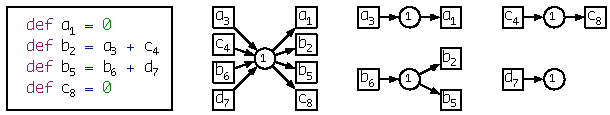
\includegraphics{figures/scope-graphs/global/example.pdf}
\end{boxedminipage}
\vspace*{-\baselineskip}
\caption{Declarations and references in global scope.}
\figurelabel{decs-and-refs}
\end{figure}


\paragraph{Duplicate declarations.}

It is possible for a scope to contain multiple references and/or
declarations with the same name.
For example, scope $1$ in \Figure{decs-and-refs} has two declarations of the
variable \pcfmcode{b}.
While the existence of multiple references is normal, multiple
declarations may give rise to multiple resolutions.
For example, the $\pcfmcode{b}_6$ reference in \Figure{decs-and-refs}
resolves to \emph{each} of the two declarations $\pcfmcode{b}_2$ and
$\pcfmcode{b}_5$.  

Typically, correct programs will not declare the same identifier
at two different locations in the same scope,
although some languages have constructs (e.g. or-patterns in OCaml~\cite{ocamlrefman}) that are most
naturally modeled this way. 
But even when the existence of multiple resolutions implies an erroneous program, 
we want the resolution
calculus to identify \emph{all} these resolutions, since IDEs and other
front-end tools need to be able to represent erroneous programs.
For example, a rename refactoring should support consistent renaming of identifiers, even in
the presence of ambiguities (see \Section{applications}).
The ability of our calculus to describe ambiguous resolutions distinguishes it
from systems, such as nominal logic~\cite{Cheney05a}, that inherently require unambiguous resolution of references. 

\vspace*{-0.5\baselineskip}

\subsection{Lexical Scope}

We model lexical scope by means of the \emph{parent} relation on scopes.
In a well-formed scope graph, each scope has at most one parent and the parent
relation is well-founded.
Formally, the partial function $\P{\_}$ maps a scope $S$ to its \emph{parent}
scope $\P{S}$.
Given a scope graph with parent relation we can define the notion of
\emph{reachable} and \emph{visible} declarations in a scope.

\Figure{lexical} illustrates how the parent relation is used to model common
lexical scope patterns.
Lexical scoping is typically presented through nested regions in the abstract
syntax tree, as illustrated by the nested boxes in \Figure{lexical}.
Expressions in inner boxes may refer to declarations in surrounding boxes, but
not vice versa.
Each of the scopes in the program is mapped to a scope (circle) in the scope
graph.
The three scopes correspond to the global scope, the scope for \pcfmcode{fix
f}$_2$, and the scope for \pcfmcode{fun n}$_3$.
The edges from scopes to scopes correspond to the parent relation.
The resolution paths on the right of \Figure{lexical} illustrate the consequences
of the encoding.
From reference \pcfmcode{f}$_6$ both declarations \pcfmcode{f}$_1$ and
\pcfmcode{f}$_2$ are \emph{reachable}, but from reference \pcfmcode{f}$_9$ only
declaration \pcfmcode{f}$_1$ is reachable.
In languages with lexical scoping, the redeclaration of
a variable inside a nested region typically \emph{hides} the outer
declaration.
Thus, the duplicate declaration of variable \pcfmcode{f} does not indicate
a program error in this situation
because only \pcfmcode{f}$_2$ is \emph{visible} from the scope of
\pcfmcode{f}$_6$.


\begin{figure}[t]
\begin{boxedminipage}{\hsize}
\centering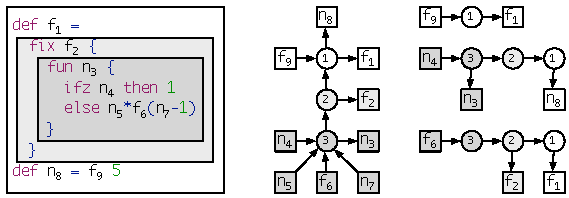
\includegraphics{figures/scope-graphs/lexical/example.pdf}
\end{boxedminipage}
\vspace*{-\baselineskip}
\caption{Lexical scoping modeled by edges between scopes in the scope
graph with example program, scope graph, and reachability paths for
references.}
\figurelabel{lexical}
\end{figure}


\paragraph{Reachability.}

The first step towards a full resolution calculus is to take into account
reachability. We redefine rule $(X_0)$ as follows: 

\begin{center}
	\infrule{X_1}{
		{\ri{x}{i}} \in \R{S_1}
        \tab
        p : S_1 \medge S_2
        \tab
  	    {\di{x}{j}} \in \D{S_2}
	}{
		p : \ri{x}{i} \resolveau \di{x}{j}
	}
\end{center}
	
\noindent
That is, $\ri{x}{i}$ in scope $S_1$ can be resolved to $\di{x}{j}$ in scope $S_2$, if
$S_2$ is \emph{reachable} from $S_1$, i.e. if $S_1 \medge S_2$.
Reachability is defined in terms of the parent relation as follows:

\begin{center}	
   \infrulenl{
		\P{S_1} = S_2
	}{
		\pstep : S_1 \edge S_2
	}
	\infrulenl{
	}{
		[] : A \medge A
	}
	\infrulenl{
		s : A \edge B
		\tab 
		p : B \medge C
	}{
		s \cdot p : A \medge C
	}
\end{center}

\noindent The parent relation between scopes gives rise to a direct edge $S_1
\edge S_2$ between child and parent scope, and $A \medge B$ is the reflexive, transitive
closure of the direct edge relation. 
In order to reason about the different ways in which a reference can be
resolved, we record the resolution path $p$. 
For example, in \Figure{lexical} reference \pcfmcode{f}$_6$ can be resolved with
path $\pstep$ to declaration \pcfmcode{f}$_2$ and with path
$\pstep\cdot\pstep$ to \pcfmcode{f}$_1$.


\paragraph{Visibility.}

Under lexical scoping, multiple possible resolutions are not problematic, as long as
the declarations reached are not declared in the same scope.
A declaration is \emph{visible} unless it is shadowed by a declaration that is
`closer by'.
To formalize visibility, we first extend reachability of scopes to
\emph{reachability of declarations}:

\display{		
	\infrule{R_2}{
                \di{x}{i} \in \D{S'}
                \tab
                p : S \medge S'
	}{
		p \cdot \dstep{\di{x}{i}} : S \reach \di{x}{i}
	}
}

\noindent
That is, a declaration $\di{x}{i}$ in $S'$ is reachable from scope $S$ ($S \reach
\di{x}{i}$), if scope $S'$ is reachable from $S$.

Given multiple reachable declarations, which one should we prefer? A reachable
declaration $\di{x}{i}$ is \emph{visible} in scope $S$ ($S \resolve \di{x}{i}$) if
there is no other declaration for the same name that is reachable
through a \emph{more specific} path:

\display{
  \infrule{V_2}{
 		p : S \reach \di{x}{i}
    \tab \tab
  	\forall j,p' (
  		 p' : S \reach \di{x}{j} \Rightarrow 
  		 \neg (p' < p)
  	)
  }{
		{p} : S \resolve \di{x}{i}
  }
}

\noindent
where the \emph{specificity ordering} $p' < p$ on paths is defined as


\vspace*{-0.5\baselineskip}

\display{
	\infrulenl{}{
		 \dstep{\_} < \pstep
	}
    \infrulenl{
		s_1 < s_2
	}{ 
		s_1\cdot p_1 < s_2 \cdot p_2
	}
	\infrulenl{
		p_1 < p_2
	}{ 
		s \cdot p_1 < s \cdot p_2
	}
}


\vspace*{-0.5\baselineskip}

\noindent
That is, a path with fewer parent transitions is more specific than a path with more
parent transitions.
This formalizes the notion that a declaration in a ``nearer'' scope shadows a
declaration in a ``farther'' scope.
	
Finally, a reference resolves to a declaration if that declaration is visible
in the scope of the reference.
	
\vspace*{-0.5\baselineskip}

\display{
   \infrule{X_2}{
		\ri{x}{i} \in \R{S}
        \tab
        p : S \resolve \di{x}{j}
	}{
		p : \ri{x}{i} \resolve \di{x}{j}
	}
}

\vspace*{-\baselineskip}

\paragraph{Example.}

In \Figure{lexical} the scope (labeled 3) containing 
reference \pcfmcode{f}$_6$ can reach two declarations for $\pcfmcode{f}$:
$\pstep\cdot\dstep{\di{\pcfmcode{f}}{2}} : S_3 \reach \di{\pcfmcode{f}}{2}$
and
$\pstep\cdot\pstep\cdot\dstep{\di{\pcfmcode{f}}{1}} : S_3 \reach
\di{\pcfmcode{f}}{1}$.
Since the first path is more specific than the second path, only \pcfmcode{f}$_2$ is
visible, i.e. $\pstep\cdot\dstep{\di{\pcfmcode{f}}{2}} : S_3 \resolve
\di{\pcfmcode{f}}{2}$.
Therefore \pcfmcode{f}$_6$ resolves to
\pcfmcode{f}$_2$, i.e. $\pstep\cdot\dstep{\di{\pcfmcode{f}}{2}} :
\ri{\pcfmcode{f}}{6} \resolve \di{\pcfmcode{f}}{2}$. 

\paragraph{Scopes, revisited.}
Now that we have defined the notions of reachability and visibility, we can
give a more precise description of the sense in which scopes ``behave
uniformly'' with respect to resolution.  For every scope $S$:
\begin{itemize}
\item Each declaration in the program is either visible
at every reference in $\R{S}$ or not visible at any reference in $\R{S}$.
\item For each reference in the program, either every declaration in $\D{S}$ is
reachable from that reference, or no declaration in $\D{S}$ is reachable 
from that reference. 
\item Every declaration in $\D{S}$ is visible at every reference in $\R{S}$.
\end{itemize}

\subsection{Imports}
\sectionlabel{imports}

Introducing modules and imports complicates the name binding picture.
Declarations are no longer visible only through the lexical context, but may be
visible through an import as well.
Furthermore, resolving a reference may require first resolving one or more
imports, which may in turn require resolving further imports, and so on. 

We model an \emph{import} by means of a reference $\ri{x}{i}$ in the set of imports
$\I{S}$ of a scope $S$. (Imports are also always references and included
in some $\R{S'}$, but not necessarily in the same scope in which they are
imports.)
We model a \emph{module} by associating a scope $S$ with
a declaration $\dsi{x}{i}{S}$.  
This associated \emph{named scope} (i.e., named by $x$) 
represents the declarations introduced by, and
encapsulated in, the module.
(We write the $:\!\!S$ only in rules where it is required; where we omit
it, the declaration may or may not have an associated scope.)
Thus, \emph{importing} entails resolving the import reference to a declaration
and making the declarations in the scope associated with that declaration
available in the importing scope.

%\paragraph{Applications.}

Note that `module' is not a built-in concept in our framework.
A module is any construct that (1) is named, (2) has an associated scope that
encapsulates declarations, and (3) can be imported into another scope.
Of course, this can be used to model the module systems of languages such as ML. 
But it can be applied to constructs that are not modules at first glance.
For example, a class in Java encapsulates class variables and methods, which are
imported into its subclasses through the `extends' clause. 
Thus, a class plays the role of module and the extends clause that of import.
We discuss further applications in \Section{coverage}.


\begin{figure}[t]
\begin{boxedminipage}{\hsize}
\centering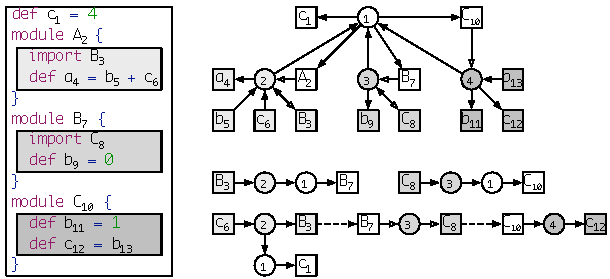
\includegraphics{figures/scope-graphs/imports/imports.pdf}
\end{boxedminipage}
\vspace*{-\baselineskip}
\caption{Modules and imports with example program, scope graph, and reachability
paths for references.}
\figurelabel{imports}
\end{figure}


\paragraph{Reachability.}

To define name resolution in the presence of imports, we first extend the
definition of reachability.
We saw above that the parent relation on scopes induces an edge $S_1 \edge
S_2$ between a scope $S_1$ and its parent scope $S_2$ in the scope graph.
Similarly, an import induces an edge $S_1 \edge S_2$ between a scope $S_1$ and
the scope $S_2$ associated with a declaration imported into $S_1$:

\vspace*{-0.5\baselineskip}

\display{
	\infrule{I_3}{
		\ri{y}{i} \in \I{S_1}  
		\tab
		p : \ri{y}{i} \resolve \dsi{y}{j}{S_2}
	}{
		\istep{\ri{y}{i}}{\dsi{y}{j}{S_2}} : S_1 \edge S_2 
	}
}

\vspace*{-0.5\baselineskip}

\noindent
Note the recursive invocation of the resolution relation on the name of the
imported scope. 

Figure~\figureref{imports} illustrates extensions to scope graphs and paths
to describe imports.
Association of a name to a scope is indicated by an open-headed arrow from the
name declaration box to the scope circle. (For example, scope 2 is associated to
declaration $\pcfmcode{A}_2$.)  An import into a scope is indicated by 
an open-headed arrow from the scope circle to the import name reference box. 
(For example, scope 2 imports the contents of the scope associated to 
the resolution of reference $\pcfmcode{B}_3$; note that 
since $\pcfmcode{B}_3$ is also a reference within scope 2, there is also an ordinary
arrow in the opposite direction, leading to a double-headed arrow in the scope graph.)
Edges in reachability paths representing the resolution of imported
scope names to their definitions are drawn dashed. (For example, reference
$\pcfmcode{B}_3$ resolves to declaration $\pcfmcode{B}_7$, which has associated
scope 3.)  The paths at the bottom right of the figure illustrate that 
the scope (labeled 2) containing reference $\pcfmcode{c}_6$ 
can reach two declarations for $\pcfmcode{c}$: 
$\pstep\cdot\dstep{\di{\pcfmcode{c}}{1}} : S_2 \reach \di{\pcfmcode{c}}{1}$
and $\istep{\ri{\pcfmcode{B}}{3}}{\dsi{\pcfmcode{B}}{7}{S_3}}\cdot
\istep{\ri{\pcfmcode{C}}{8}}{\dsi{\pcfmcode{C}}{10}{S_4}}\cdot
\dstep{\di{\pcfmcode{c}}{12}} : S_2 \reach \di{\pcfmcode{c}}{12}$,
making use of the subsidiary resolutions
$\ri{\pcfmcode{B}}{3} \resolve \di{\pcfmcode{B}}{7}$ and
$\ri{\pcfmcode{C}}{8} \resolve \di{\pcfmcode{C}}{10}$.


\begin{wrapfigure}[22]{r}{2.5cm}
\vspace*{-0.9\baselineskip}
\begin{lstlisting}
def a$_1$ = ...
module A$_2$ {
  def a$_3$ = ... 
  def b$_4$ = ...
}
module C$_5$ {
  import A$_6$
  def b$_7$ = a$_8$
  def c$_9$ = b$_{10}$
}
\end{lstlisting}
\vspace*{-\baselineskip}
\caption{Parent vs Import}
\figurelabel{parent-vs-import}
\smallskip
% \end{wrapfigure}
% \begin{wrapfigure}[12]{r}{2.5cm}
%\vspace*{-1.7\baselineskip}
\begin{lstlisting}
def a$_1$ = ...
module B$_2$ {
}
module C$_3$ {
  def a$_4$ = ...
  module D$_5$ {
    import B$_6$
    def e$_7$ = a$_8$
  }
}
\end{lstlisting}
\vspace*{-\baselineskip}
\caption{Parent of import}
\figurelabel{parent-of-import}
\end{wrapfigure} 

\paragraph{Visibility.}

Imports cause new kinds of ambiguities in resolution paths, which require
extension of the visibility policy.

The first issue is illustrated by \Figure{parent-vs-import}.
In the scope of reference \pcfmcode{b}$_{10}$ we can reach declaration
\pcfmcode{b}$_7$ with path $\dstep{\di{\pcfmcode{b}}{7}}$ and
declaration \pcfmcode{b}$_4$ with path
$\istep{\ri{A}{6}}{\dsi{A}{2}{S_A}}\cdot\dstep{\di{\pcfmcode{b}}{4}}$
(where $S_A$ is the scope named by declaration $A_2$).
We resolve this conflict by extending the specificity order with the rule
$\dstep{\_} < \istep{\_}{\_}$.
That is, local declarations override imported declarations.
Similarly, in the scope of reference \pcfmcode{a}$_8$ we can reach declaration
\pcfmcode{a}$_1$ with path $\pstep\cdot\dstep{\di{\pcfmcode{a}}{1}}$ and
declaration \pcfmcode{a}$_3$ with path
$\istep{\ri{A}{6}}{\dsi{A}{2}{S_A}}\cdot\dstep{\di{\pcfmcode{a}}{3}}$. 
We resolve this conflict by extending the specificity order with the rule
$\istep{\_}{\_} < \pstep$.
That is, resolution through imports is preferred over resolution through
parents. 
In other words, declarations in imported modules override declarations in
lexical parents.




The next issue is illustrated in \Figure{parent-of-import}. 
In the scope of reference \pcfmcode{a}$_8$ we can reach declaration
\pcfmcode{a}$_4$ with path $\pstep\cdot\dstep{\di{\pcfmcode{a}}{4}}$ and
declaration \pcfmcode{a}$_1$ with path $\pstep\cdot\pstep\cdot\dstep{\di{\pcfmcode{a}}{1}}$.
The specificity ordering guarantees that only the first of these is visible, giving
the resolution we expect.  However, with the rules as stated so far, there
is another way to reach \pcfmcode{a}$_1$, via the path
$\istep{\ri{\pcfmcode{B}}{6}}{\dsi{\pcfmcode{B}}{2}{S_B}}\cdot
\pstep\cdot\dstep{\di{\pcfmcode{a}}{1}}$.
That is, we first import module \pcfmcode{B}, and then go to its lexical 
parent, where we find the declaration.  In other words,
when importing a module, we 
import not just its declarations, but all declarations in its lexical context.
This behavior seems undesirable; to our knowledge, no real languages exhibit it. 
To rule out such resolutions, we define a well-formedness predicate $\WF(p)$
that requires paths $p$ to be of the form $\pstep^* \cdot \istep{\_}{\_}^*$, 
i.e. forbidding the use of parent steps after one or more import
steps. We use this predicate to restrict the reachable declarations relation by
only considering scopes reachable through a well-formed path:

\display{
	\infrule{R_3}{
		\di{x}{i} \in \D{S'}
		\tab
		p : S \medge S'
		\tab 
		\WF(p)
	}{
		p \cdot \dstep{\di{x}{i}} : S \reach \di{x}{i}
	}
}	

\noindent
The complete definition of well-formed paths and specificity order on paths is
given in \Figure{order}.
In \Section{extensions} we discuss how alternative visibility policies can be
defined by just changing the well-formedness predicate and specificity order.

\begin{figure}[t]
\begin{boxedminipage}{\hsize}
$$
\inferrule*{  
  \inferrule*{
    \inferrule*{
      \dsi{A}{2}{S_{A_2}} \in \D{S_{A_1}} 
      \tab
      \inferrule*{
        \ri{A}{4} \in \I{S_{root}}
        \tab
        \inferrule*{
          \ri{A}{4} \in \R{S_{root}}
          \\
          \dsi{A}{1}{S_{A_1}} \in \D{S_{root}}
        }{
          \ri{A}{4} \resolve \dsi{A}{1}{S_{A_1}}
        }
      }{
        S_{root} \edge S_{A_1} \tab (*)
      }
    }{
      S_{root} \reach \dsi{A}{2}{S_{A_2}}  
    }
  }{
    \ri{A}{4} \in \R{S_{root}}
    \tab 
    S_{root} \resolve \dsi{A}{2}{S_{A_2}}
  }
}{
\ri{A}{4} \resolve \dsi{A}{2}{S_{A_2}}
}
$$
\end{boxedminipage}
\vspace*{-\baselineskip}
\caption{Derivation for $\ri{A}{4} \resolve \dsi{A}{2}{S_{A_2}}$ in a calculus without import tracking.}
\figurelabel{self-import-derivation}
\end{figure}

\begin{wrapfigure}[20]{r}{2.6cm}
\vspace*{-.7\baselineskip}
\begin{lstlisting}
module A$_1$ { 
  module A$_2$ { 
    def a$_3$ = ...
  } 
}
import A$_4$
def b$_5$ = a$_6$
\end{lstlisting}
\vspace*{-\baselineskip}
\caption{Self import}
\figurelabel{self-import}
\medskip

% \end{wrapfigure}
% \begin{wrapfigure}[12]{r}{2.5cm}
%\vspace*{-\baselineskip}
\begin{lstlisting}
module A$_1$ {
  module B$_2$ { 
    def x$_3$ = 1 
  }
}
module B$_4$ {
  module A$_5$ { 
    def y$_6$ = 2 
  }
}
module C$_7$ {
  import A$_8$
  import B$_9$
  def z$_{10}$ = x$_{11}$ 
          + y$_{12}$
}
\end{lstlisting}
\vspace*{-\baselineskip}
\caption{Anomalous resolution}
\figurelabel{anomalous}
\end{wrapfigure}


\paragraph{Seen imports.}

Consider the example in \Figure{self-import}. 
Is declaration \pcfmcode{a}$_3$ reachable in the scope of reference
\pcfmcode{a}$_6$?
This reduces to the question whether the import of \pcfmcode{A}$_4$ can resolve to
module \pcfmcode{A}$_2$.
Surprisingly, it can, in the calculus as discussed so far, as shown by the
derivation in \Figure{self-import-derivation} (which takes a few shortcuts).
The conclusion of the derivation is that 
$\ri{A}{4} \resolve \dsi{A}{2}{S_{A_2}}$.
This conclusion is obtained by \emph{using the import at \pcfmcode{A}$_4$}
to conclude at step (*) that $S_{root} \edge S_{A_1}$, i.e. that the body of
module \pcfmcode{A}$_1$ is reachable!
In other words, the import of \pcfmcode{A}$_4$ is used in its own
resolution.  Intuitively, this is nonsensical.

To rule out this kind of behavior we extend the calculus to keep track of the
set of \emph{seen imports} $\seeni$ using judgements of the form 
$\seeni \vdash p : \ri{x}{i} \resolve \di{x}{j}$. 
We need to extend all rules to pass the set $\seeni$, but only the rules
for resolution and import are truly affected:

%\vspace*{-.5\baselineskip}

\display{
	\infrule{X}{
		\ri{x}{i} \in \R{S}
        \tab
        \{ \ri{x}{i} \} \cup \seeni \vdash p : S \resolve \di{x}{j}
	}{
		\seeni \vdash p : \ri{x}{i} \resolve \di{x}{j}
	}
}

\vspace*{-1.5\baselineskip}

\display{
	\infrule{I}{
		\ri{y}{i} \in \I{S_1}\setminus\seeni  
		\tab
		\seeni \vdash p : \ri{y}{i} \resolve \dsi{y}{j}{S_2}
	}{
		\seeni \vdash \istep{\ri{y}{i}}{\dsi{y}{j}{S_2}} : S_1 \edge S_2 
	}
}

%\vspace*{-0.5\baselineskip}


With this final ingredient, we reach the full calculus in \Figure{rescalc}.
It is not hard to see that the resolution relation is well-founded. The only
recursive invocation (via the $I$ rule) uses a strictly larger set $\seeni$
of seen imports (via the $X$ rule); since the set $\R{G}$ is finite, $\seeni$ cannot
grow indefinitely.

\paragraph{Anomalies.}

Although the calculus produces the desired resolutions for a wide variety
of real language constructs, its behavior can be surprising on corner cases.
Even with the ``seen imports'' mechanism, it is still possible for
a single derivation to resolve a given import in two different ways, leading to 
unintuitive results.  For example, in the program in \Figure{anomalous},
\pcfmcode{x}$_{11}$ can resolve to \pcfmcode{x}$_3$ and
\pcfmcode{y}$_{12}$ can resolve to \pcfmcode{y}$_6$. (Derivations left as an exercise
to the curious reader!)  
In our experience, phenomena like this occur only in the presence of
mutually-recursive imports; to our knowledge, no real language has these
(perhaps for good reason).  We defer deeper exploration of these anomalies
to future work.


%%%%%%%%%%%%%%%%%%%%%%%%%%%%%%%%%%%%%%%%%%%%%%%%%%
\endinput
	  
\paragraph{Cyclic Import Dependencies}

\begin{lstlisting}
module A { import B }
module B { import A }
\end{lstlisting}

\begin{lstlisting}
module A {
   module B {}
}
module B {
   module A {}
}
module M {
   import C;
   import D;   
   module C { import A };
   module D { import B }
} 
\end{lstlisting}

The resolution of {\tt A} can use {\tt import B} through {\tt import D} and the resolution of {\tt B} can use {\tt import A} through {\tt import C}.
Thus with seen imports both imports resolve to the innermost modules.
The following program also has the same behavior:

\begin{lstlisting}
module A {
   module B {}
}
module B {
   module A {}
}
module M {
   import C.D; 
   module C {     
      import A 
      module D { 
         import B }
      }
   }
} 
\end{lstlisting}




\paragraph{}


Notice that the identifier of an import can have a different enclosing scope than the
scope for which it is an import. 

That is, the implication $x^p \in \I{S}
\Rightarrow x^p \in \R{S}$ does \emph{not} hold. 
For example, in \Figure{includes}, the identifier $B_1$ is a
reference in scope 3, but an import in scope 2.

\subsection{Errors in Resolved Scope Graph}

\parindent0pt
\parskip0.5\baselineskip
\TODO{remove parindent/parskip commands}
	
problems in programs that lead to errors in scope graph

how this would be presented in the IDE

unresolved reference

ambiguous / conflicting resolution

quick fixing




\subsection{Construction of Scope Graph}

\TODO{algorithm for construction of scope graph for LM programs}


A scope often corresponds to a node in the AST, but this is not necessarily the
case. 

how one arrives at the set of program points 

The very challenge of formulating a theory of name resolution is to describe the
rules

a scope is smaller than a traditional scope



Languages use scoping constructs to restrict the visibility of names.
A name declared in a scope is not visible outside that scope.






	\subsection{Variants}
\sectionlabel{extensions}

The resolution calculus presented so far reflects a number of binding policy decisions.
For example, we enforce imports to be transitive and
local declarations to be preferred over imports.
However, not every language behaves like this. We now present how
other common behaviors can easily be represented with slight modifications of
the calculus.
Indeed, the modifications do not have to be done on the calculus itself (the
$\edge$, $\medge$, $\reach$ and $\resolve$ relations) but can simply be encoded
in the $\WF$ predicate and the $<$ ordering on paths.

\paragraph{Reachability policy.}

Reachability policies define how a reference can access a particular
definition, i.e. what rules can be used during the resolution. We 
can change our reachability policy by modifying the $\WF$ predicate. 
For example, if we want to rule out transitive imports, we can change $\WF$ to be
\vspace*{-0.4\baselineskip}
$$ \WF(p) \Leftrightarrow p \in \pstep^* \cdot \istep{\_}{\_}? \vspace*{-0.4\baselineskip}
$$ 
where $?$ denotes the \emph{at most one} operation on regular expressions.
Therefore, an import can only be used once at the end of the chain of scopes.

For a language that supports both transitive and non-transitive imports, we can add a
label on references corresponding to imports.
If $\r{x}$ is a reference representing a non-transitive import and $\tr{x}$
a reference corresponding to a transitive import, then the $\WF$ predicate
simply becomes:
\vspace*{-0.4\baselineskip}
$$ \WF(p) \Leftrightarrow p \in \pstep^* \cdot \istep{\tr{\_}}{\_}^*\cdot
\istep{\r{\_}}{\_}? \vspace*{-0.4\baselineskip}$$ 

\begin{wrapfigure}[7]{r}{0.2\textwidth}
\vspace*{-0.7\baselineskip}
\begin{lstlisting}[language=PCFM]
module A$_1$ {
  def x$_2$ = 3
}
module B$_3$ {
  include A$_4$;
  def x$_5$ = 6;
  def z$_6$ = x$_7$
} 
\end{lstlisting}
\vspace*{-0.7\baselineskip}
\caption{Include}
\label{fig:include}
\end{wrapfigure}

\noindent Now no import can occur after the use of a non-transitive one.

Similarly, we can modify the rule to handle the \emph{Export} declaration in 
Coq, which forces transitivity (a resolution can always use an exported module
even after importing from a non-transitive one).
Assume $\r{x}$ is a reference representing a non-transitive import and
$\er{x}$ a reference corresponding to an export; then we can use the
following predicate:

\vspace*{-0.4\baselineskip}
$$ \WF(p) \Leftrightarrow p \in \pstep^* \cdot \istep{\r{\_}}{\_}? \cdot
\istep{\er{\_}}{\_}^*\vspace*{-0.4\baselineskip}
 $$


\paragraph{Visibility policy.}

We can modify the visibility policy, i.e. how
resolutions shadow each other, by changing the definition of the specificity ordering.
For example, we might want imports to 
act like textual inclusion, so the declarations in the included module have 
the same precedence as local declarations. This is similar to Standard ML's \pcfmcode{include}
mechanism.
In the program in \Figure{include}, the reference \pcfmcode{x}$_7$ should be treated
as having duplicate resolutions, to either \pcfmcode{x}$_5$ or \pcfmcode{x}$_2$;
the former should not hide the latter.
To handle this situation, we can drop the rule
$\dstep{\_} < \istep{\_}{\_}$ so that definitions and references
will get the same precedence, and a definition will not shadow an imported
definition.
To handle both \pcfmcode{include} and ordinary imports, we can once again differentiate
the references, and define different ordering rules depending on the reference used
in the import step.

% export as in Coq

	%\newpage\clearpage		
	\section{Coverage}
\sectionlabel{coverage}

To what extent does the scope graph framework cover name binding systems that live in the
world of real programming languages? It is not possible to \emph{prove} complete
coverage by the framework, in the sense of being able to encode all possible
name binding systems that exist or may be designed in the future.
(Indeed, given that these systems are typically implemented in compilers
with algorithms in Turing-complete programming languages, the framework is likely
\emph{not} to be complete.)
However, we believe that our approach handles many lexically-scoped languages.
The design of the framework was informed by an investigation of a wide range of
name binding patterns in existing languages, their (attempted) formalization in
the NaBL name binding language \cite{KatsV10,KonatKWV12}, and their encoding in scope
graphs.
In this section, we discuss three such examples: \pcfmcode{let} bindings, qualified names,
and inheritance in Java.
This should provide the reader with a good sense of how name binding patterns
can be expressed using scope graphs.
Appendix  \refcoverageappendix\techrep{~of \cite{TUD-SERG-2015-001-local}}{} provides further examples,
including definition-before-use, compilation units and packages in Java, and namespaces and partial classes in
C\#. 

\begin{figure}[t]
\begin{boxedminipage}{\hsize}
\centering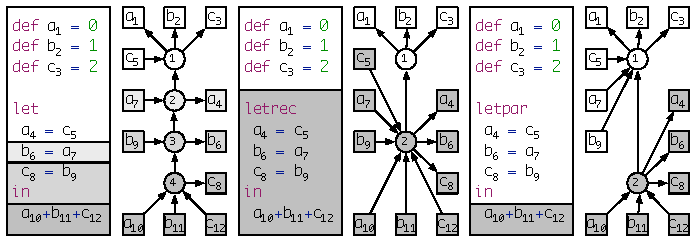
\includegraphics{figures/scope-graphs/lets/all.pdf}
\end{boxedminipage}
% \vspace{1ex}
% \hrule
\vspace*{-\baselineskip}
\caption{Example LM programs with sequential, recursive, and parallel \pcfmcode{let}, and
their encodings as scope graphs.}
\figurelabel{lm:lets}
\end{figure}

\paragraph{Let bindings.}

The several flavors of \pcfmcode{let} bindings in languages such as ML, Haskell, and
Scheme do not follow the unary lexical binding pattern in which the binding
construct dominates the abstract syntax tree that makes up its scope.
The LM language from \Figure{pcfm:grammar} has three flavors of \pcfmcode{let} bindings:
sequential, recursive, and parallel \pcfmcode{let}, each with a list of bindings and
a body expression.
\Figure{lm:lets} shows the encoding into scope graphs for each of the constructs
and makes precise how the bindings are interpreted in each flavour.
In the recursive \pcfmcode{letrec}, the bindings are visible in all initializing
expressions, so a single scope suffices for the whole construct.
In the sequential \pcfmcode{let}, each binding is visible in the
\emph{subsequent} bindings, but not in its own initializing expression. This
requires the introduction of a new scope for each binding.
In the parallel \pcfmcode{letpar}, the variables being bound are not
visible in any of the initializing expressions, but only in the body.
This is expressed by means of a single scope (2) in which the bindings are
declared; any references in the initializing expressions are associated to the
parent scope (1).

\begin{figure}[t]
\begin{minipage}[b]{0.49\textwidth}
\begin{boxedminipage}{\hsize}
\hspace*{-0.3cm}
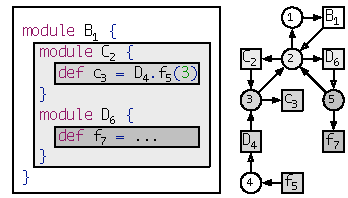
\includegraphics{figures/scope-graphs/qualified/example3.pdf}
\end{boxedminipage}
\caption{Example LM program with partially-qualified name.}
\figurelabel{lm:qualified}
\end{minipage}
\begin{minipage}[b]{0.49\textwidth}
\begin{boxedminipage}{\hsize}
\hspace*{-1.5mm}
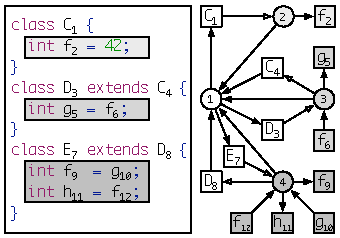
\includegraphics{figures/scope-graphs/inheritance/inheritance.pdf}
\end{boxedminipage}
\caption{Class inheritance in Java modeled by import edges.}
\figurelabel{java:inh}
\end{minipage}
\end{figure}



% \begin{wrapfigure}[11]{r}{0.51\textwidth}
% \vspace*{-2\baselineskip}
% \begin{boxedminipage}{\hsize}
% \centering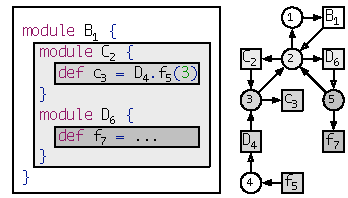
\includegraphics{figures/scope-graphs/qualified/example3.pdf}
% \end{boxedminipage}
% \caption{Example LM program with partially-qualfied name.}
% \figurelabel{lm:qualified}
% \end{wrapfigure}

\paragraph{Qualified names.}

Qualified names refer to declarations in named scopes outside the lexical scoping.
They can be either used as simple references or as imports.
For example, fully-qualified names of Java classes can be used to refer to (or import) classes
  from other packages.
While fully-qualified names allow navigating named scopes from the root scope,
partially-qualified names give access to lexical subscopes, 
  which are otherwise hidden from lexical parent scopes.

The LM program in \Figure{lm:qualified} uses a
partially-qualified name \pcfmcode{D.f} to access function \pcfmcode{f} in submodule \pcfmcode{D}.
We can model this pattern using an anonymous scope (4),
which is not linked to the lexical context. The relative name
(\pcfmcode{f}$_5$) is a reference in the anonymous scope.
We add the qualifying scope name (\pcfmcode{D}$_4$) as an import in the
anonymous scope. 
  
%\TODO{The declaration of a subpackage is never in scope.}

%\TODO{aliases: should probably be postponed to future work}

% \begin{wrapfigure}[14]{r}{0.51\textwidth}
% \vspace*{-1\baselineskip}
% \begin{boxedminipage}{\hsize}
% \centering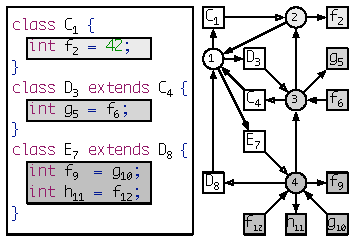
\includegraphics{figures/scope-graphs/inheritance/transitive.pdf}
% \end{boxedminipage}
% \caption{Class inheritance in Java modeled by import edges.}
% \figurelabel{java:inh}
% \end{wrapfigure}

\paragraph{Inheritance in Java.}

%As we alluded to in \Section{imports}, the concepts of named scopes and imports
%in the scope graph framework can be used to model more than just language
%constructs called `module'.
We can model
inheritance in object-oriented languages 
with named scopes and imports.
For example, \Figure{java:inh} shows a hierarchy of three Java classes.
Class \javacode{C} declares a field \javacode{f}.
Class \javacode{D} extends \javacode{C} and inherits its field \javacode{f}.   
Class \javacode{E} extends \javacode{D}, inheriting the fields of \javacode{C} and \javacode{D}.
Each class name is a declaration in the same package scope (1),
  and associated with the scope of its class body.
Inheritance is modeled with imports: a subclass body scope contains an import referring to its super class, making the declarations in the super class reachable from the body. In the example, the scope (4) representing the body of class \javacode{E} contains an import referring to its super class \javacode{D}. Using this import, \javacode{g}$_{10}$ correctly resolves to \javacode{g}$_{5}$ . Since local declarations hide imported declarations, \javacode{f}$_{12}$ also refers correctly to the local declaration \javacode{f}$_{9}$, which hides the transitively imported \javacode{f}$_{2}$.
Note that since a scope can contain several imports, encoding multiple inheritance uses exactly the same principle.

	%\newpage\clearpage
	%\newpage\clearpage
        \section{Scope Graph Construction}
\sectionlabel{construction}


%% \newcommand{\semop}[1]{[\![ #1 ]\!]}
%% \newcommand{\sem}[2]{\semop{#1}(#2)}
%% % PCFM code for math mode
%% \newcommand{\semcode}[1]{\text{\pcfmcodefig{#1}}}
%% % Formula for regular interpretation translation
%% \newcommand{\semf}[4]{
%%  $\semop{#1}(#2) = #3$\\
%% \smallskip
%% \qquad$\text{\textsf{where}} \ #4 $
%% }
%% \newcommand{\semfs}[4]{
%% $\sems{#1}{#2} = #3$\\
%% \smallskip
%% \qquad$\text{\textsf{where}} \ #4 $
%% }
%% \newcommand{\semfp}[5]{
%% $\semp{#1}{#2}{#3} = #4$\\
%% \smallskip
%% \qquad$\text{\textsf{where}} \ #5 $
%% }

%% \newcommand{\semfline}[4]{
%%  $\semop{#1}(#2) = #3 \quad\text{\textsf{where}} \ #4 $
%% }

%% \newcommand{\semp}[3]{\semop{#1}^p(#2,#3)}
%% \newcommand{\sems}[2]{\semop{#1}^s(#2)}

%% \newcommand{\sappend}{\ \text{+=}\ }
%% \newcommand{\sdefine}{\ \text{:=}\ }

\newcommand{\sema}[3]{
\semop{#1}^{#2}_{#3}
}

%\newcommand{\snew}[1]{\text{\textsf{newscope}}\{\text{\textsf{par=}}#1\}}
\newcommand{\snew}[1]{\text{\textsf{new}}_{#1}}
\newcommand{\sret}[1]{\text{\textsf{ret}}(#1)}

\newcommand{\semeqn}[4]{
$\sema{#1}{#2}{#3}$ & $\sdefine$ & ${#4}$}

\newcommand{\slet}{\text{\textsf{let }}}
\renewcommand{\sin}{\text{\textsf{ in }}}

\newcommand{\myskip}{\\[4.5pt]}

\begin{figure}[tb]
%\fbox{
\begin{boxedminipage}{\hsize}
\begin{tabular}{rcl}
\semeqn{\semcode{ds}}{prog}{}
{
\slet S \sdefine \snew{\perp} \sin
\sema{\semcode{ds}}{recd}{S}
}
\myskip
\semeqn{\semcode{d ds}}{recd}{S}
{
\sema{\semcode{d}}{dec}{S}; 
\sema{\semcode{ds}}{recd}{S}
}
\\
\semeqn{}{recd}{S}{
()
}
\myskip
\semeqn{\semcode{module x}_i \semcode{ \{ds\}}}{dec}{S}
{
\slet S' \sdefine \snew{S} \sin 
\D{S} \sappend \dsi{x}{i}{S'}; 
\sema{\semcode{ds}}{recd}{S'}
}
\\
\semeqn{\semcode{import xs}}{dec}{S}
{
\sema{\semcode{xs}}{rqid}{S};
\sema{\semcode{xs}}{iqid}{S}
}
\\
\semeqn{\semcode{def x}_i\semcode{\ = e}}{dec}{S}
{
\D{S} \sappend \di{x}{i};
\sema{\semcode{e}}{exp}{S}
}
\myskip
\semeqn{\semcode{xs}}{exp}{S}
{
\sema{\semcode{xs}}{rqid}{S}
}
\\
\semeqn{\semcode{\(fun | fix\) x}_i\semcode{ \{e\}}}{exp}{S}
{
\slet S' \sdefine \snew{S} \sin
\D{S'} \sappend \di{x}{i};
\sema{\semcode{e}}{exp}{S'}
}
\\
\semeqn{\semcode{letrec bs in e}}{exp}{S}
{
\slet S' \sdefine \snew{S} \sin 
\sema{\semcode{bs}}{recb}{S'};
\sema{\semcode{e}}{exp}{S'}
}
\\
\semeqn{\semcode{letpar bs in e}}{exp}{S}
{
\slet S' \sdefine \snew{S} \sin 
\sema{\semcode{bs}}{parb}{(S,S')};
\sema{\semcode{e}}{exp}{S'}
}
\\
\semeqn{\semcode{let bs in e}}{exp}{S}
{
\slet S' \sdefine \sema{bs}{seqb}{S} \sin
\sema{\semcode{e}}{exp}{S'}
}
\\
\semeqn{\semcode{e}_1\ \semcode{e}_2}{exp}{S}
{
\sema{\semcode{e}_1}{exp}{S};
\sema{\semcode{e}_2}{exp}{S}
}
\\
\semeqn{\semcode{e}_1 \oplus \semcode{e}_2}{exp}{S}
{
\sema{\semcode{e}_1}{exp}{S};
\sema{\semcode{e}_2}{exp}{S}
}
\\
\semeqn{\semcode{n}}{exp}{S}
{
()
}
\myskip
\semeqn{\semcode{x}_i\semcode{.xs}}{rqid}{S}
{
\R{S} \sappend \ri{x}{i};
\slet S' \sdefine \snew{\perp} \sin 
\I{S'} \sappend \ri{x}{i};
\sema{xs}{rqid}{S'}
}
\\
\semeqn{\semcode{x}_i}{rqid}{S}
{
\R{S} \sappend \ri{x}{i}
}
\myskip
\semeqn{\semcode{x}_i\semcode{.xs}}{iqid}{S}
{
\sema{xs}{iqid}{S}
}
\\
\semeqn{\semcode{x}_i}{iqid}{S}
{
\I{S} \sappend \ri{x}{i}
}
\myskip
\semeqn{\semcode{x}_i\semcode{\ = e; bs}}{recb}{S}
{
\D{S} \sappend \di{x}{i};
\sema{\semcode{e}}{exp}{S};
\sema{\semcode{bs}}{recb}{S}
}
\\
\semeqn{}{recb}{S}
{
()
}
\myskip
\semeqn{\semcode{x}_i\semcode{\ = e; bs}}{parb}{(S,S')}
{
\D{S'} \sappend \di{x}{i};
\sema{\semcode{e}}{exp}{S};
\sema{\semcode{bs}}{parb}{(S,S')}
}
\\
\semeqn{}{parb}{(S,S')}
{
()
}
\myskip
\semeqn{\semcode{x}_i\semcode{\ = e; bs}}{seqb}{S}
{
\sema{\semcode{e}}{exp}{S};
\slet S' \sdefine \snew{S} \sin
\D{S'} \sappend \di{x}{i};
\sret{S'}
}
\\
\semeqn{}{seqb}{S}
{
\sret{S}
}
\end{tabular}
\end{boxedminipage}
%}
% }}\smallskip
\caption{Scope graph construction for LM via syntax-directed AST traversal.}
\label{fig:lm-scopegraph-construction}
\end{figure}


The preceding sections have illustrated scope graph construction
by means of examples corresponding to various language features. 
Of course, to apply our formalism in practice, one must be able
to construct scope graphs systematically. Ultimately, we would
like to be able to specify this process for arbitrary 
languages using a generic binding specification language such
as NaBL~\cite{KonatKWV12}, but that remains future work.
Here we illustrate systematic scope graph construction for arbitrary
programs in a \emph{specific} language, LM (\Figure{pcfm:grammar}), 
via straightforward syntax-directed traversal.  

Figure~\ref{fig:lm-scopegraph-construction} describes the
construction algorithm.
For clarity of presentation, the algorithm traverses the 
program's concrete syntax; a real implementation would
traverse the program's AST.
The algorithm is presented in an {\it ad hoc} imperative language, 
explained here.  The traversal is specified as a collection of 
(potentially) mutually recursive functions, one or more for
each syntactic class of LM. Each function $f$ is
defined by a set of clauses $\sema{\mbox{\it{pattern}}}{f}{args}$.
When $f$ is invoked on a term, the clause whose {\it{pattern}} matches
the term is executed.  Functions may also take additional arguments $args$. 
Each clause body consists of a sequence of
statements separated by semicolons. Functions can optionally return a value
using $\sret{}$.
The $\slet$ \hspace*{-0.6em} statement binds 
a metavariable in the remainder of the clause body.
An empty clause body is written $()$.

The algorithm is initiated by invoking $\sema{\_}{prog}{}$ on an entire LM
program. Its net effect is to produce a scope graph via a sequence of
imperative operations. 
The construct $\snew{P}$ creates a new scope $S$ with parent $P$ 
(or no parent if  $p = \perp$) and
empty sets $\D{S}$, $\R{S}$, and $\I{S}$. 
These sets are subsequently populated using the
$\sappend$ operator, which extends a set imperatively.
The program scope graph is simply the set of scopes that have been created
and populated when the traversal terminates.




	\section{Resolution Algorithm}
\sectionlabel{resalg}

The calculus of \Section{rescalc} gives a precise definition of resolution.
In principle, we can search for derivations in the calculus 
to answer questions such as ``Does this variable
reference resolve to this declaration?'' or ``Which variable declarations
does this reference resolve to?''  But automating this search process is not trivial, 
because of the need for back-tracking and 
because the paths in reachability derivations can have cycles (visiting
the same scope more than once), and hence can grow arbitrarily long.

In this section we describe a deterministic and terminating
\emph{algorithm} for computing resolutions,
which provides a practical basis for implementing tools based on scope graphs,
and prove that it is sound and complete with respect to the calculus.
This algorithm also connects the calculus, which talks about
resolution of a single variable at a time, to more conventional descriptions of
binding which use ``environments'' or ``contexts'' to describe \emph{all}
the visible or reachable declarations accessible from a program location.

For us, an \emph{environment} is just a set of declarations $\di{x}{i}$. 
This can be thought of as a function from identifiers to (possible empty) 
sets of declaration positions.  (In this paper, we leave the representation 
of environments abstract; in practice, one would use a hash table or other
dictionary data structure.) We construct an atomic environment corresponding
to the declarations in each scope, 
and then combine atomic environments to describe the sets of 
reachable and visible declarations resulting from the parent and import 
relations. The key operator for combining environments is {\it shadowing},
which returns the union of the declarations in two environments restricted so
that if a variable $x$ has any declarations in the first environment, no
declarations of $x$ are included from the second environment.  More formally:


\begin{figure}[t]
\renewcommand{\S}{\mathcal{S}}
\begin{boxedminipage}{\hsize}
\vspace*{-0.5\baselineskip}
$$
\begin{array}{ll}
  \Res{\seeni}{\ri{x}{i}} & := \{ \di{x}{j} \mid \exists S\ s.t.\ \ri{x}{i} \in \R{S} \wedge \di{x}{j} \in \Env{V}{\{\ri{x}{i}\} \cup \seeni}{\emptyset}{S} \} \smallskip  \\
  \Env{V}{\seeni}{\seens}{S}  & := \Env{L}{\seeni}{\seens}{S} \triangleleft \Env{P}{\seeni}{\seens}{S} \smallskip\\
 \Env{L}{\seeni}{\seens}{S} & := \Env{D}{\seeni}{\seens}{S} \triangleleft \Env{I}{\seeni}{\seens}{S} \smallskip\\
 \Env{D}{\seeni}{\seens}{S} &:= \left\{
    \begin{array}{l}
      \emptyset  \text{ if } S\in\seens\\
      \D{S}\smallskip\\
    \end{array}
 \right.\smallskip\\
 \Env{I}{\seeni}{\seens}{S} &:= \left\{
    \begin{array}{l}
      \emptyset  \text{ if } S\in\seens\\
      \bigcup \left\{ \Env{L}{\seeni}{\{S\}\cup\seens}{S_y} \mid \ri{y}{i} \in \I{S} \setminus 
\seeni \wedge \dsi{y}{j}{S_y} \in \Res{\seeni}{\ri{y}{i}}\right\}\smallskip\\
%       \bigcup \limits_{\r{y} \in \I{S} \setminus \seeni} 
%          \left\{ \Env{L}{\seeni}{\{S\}\cup\seens}{S_y} \mid \ds{y}{S_y} \in \Res{\seeni}{\r{y}}\right\}\smallskip\\
    \end{array}
 \right.\smallskip\\
 \Env{P}{\seeni}{\seens}{S} & := \left\{
    \begin{array}{l}
      \emptyset  \text{ if } S\in\seens\\
      \Env{V}{\seeni}{\{S\}\cup\seens}{\P{S}}
    \end{array}
 \right.\smallskip\\
\end{array}\medskip
$$
\vspace*{-1.5\baselineskip}
\end{boxedminipage}
\vspace*{-\baselineskip}
\caption{Resolution algorithm}
\label{fig:resalg}
\end{figure}


% \vspace*{-0.3\baselineskip}

\begin{definition}[Shadowing] For any environments $E_1$, $E_2$, we write:\\
\centerline{$E_1 \hiding E_2 := E_1 \cup \{ \di{x}{i} \in E_2 \mid  \nexists\ \di{x}{i'} \in
E_1\}$}
\end{definition}

%\vspace*{-.2\baselineskip}

\noindent
Figure~\ref{fig:resalg} specifies an algorithm $\Res{\seeni}{\ri{x}{i}}$
for resolving a reference $\ri{x}{i}$
to a set of corresponding declarations $\di{x}{j}$.
Like the calculus,
the algorithm avoids trying to use an import to resolve itself
by maintaining a set $\seeni$ of ``already seen'' imports.
The algorithm works by computing the full environment $\Env{V}{\seeni}{\seens}{S}$ 
of declarations that are visible in the scope $S$ containing $\ri{x}{i}$, and 
then extracting just the declarations for $x$. The full environment, in turn,
is built from the more basic environments $\Envu{D}$ of immediate declarations,
$\Envu{I}$ of imported declarations, and $\Envu{P}$ of lexically enclosing declarations,
using the shadowing operator.  The order of construction matches both the $\WF$ restriction
from the calculus, which prevents the use of parent after an import, and  the path ordering $<$,
which prefers immediate declarations over imports and imports over 
declarations from the parent scope.  
(Note that the algorithm does \emph{not} work for the variants of $\WF$
and $<$ described in \Section{extensions}.)
%The algorithm is naturally implemented by 
%constructing the various environments lazily. 
A key difference from the calculus is that the shadowing operator is applied at
each stage in environment construction, rather than applying the visibility 
criterion just once at the ``top level'' as in calculus rule $V$. 
This difference is a natural consequence of the fact that the algorithm computes
sets of declarations rather than full derivation paths, so it does not maintain
enough information to delay the visibility computation.

\paragraph{Termination} The algorithm is terminating using the well-founded
lexicographic measure  $(|\R{\G} \setminus \seeni|,|\S{\G} \setminus \seens|)$.
Termination is straightforward by unfolding the calls to $Res$ in $\Envu{I}$ and then 
inlining the definitions of $\Envu{V}$ and $\Envu{L}$: this gives an equivalent algorithm 
in which the measure strictly decreases at every recursive call.

\subsection{Correctness of Resolution Algorithm}

The resolution algorithm is sound and complete
with respect to the calculus. 
\begin{theorem}
\label{theorem:correctness}
$\forall\ \seeni, \ri{x}{i}, j, (\di{x}{j}\in \Res{\seeni}{\ri{x}{i}}) 
\iff (\exists p\ s.t.\ \seeni \vdash p : \ri{x}{i} \resolve \di{x}{j})$.
\end{theorem}

We sketch the proof of this theorem here; 
details of the supporting lemmas and proofs are in Appendix \refproofappendix\techrep{~of
\cite{TUD-SERG-2015-001-local}}{}.
To begin with, we must deal with the fact that the calculus can
generate reachability derivations with cycles,
but the algorithm does not follow cycles.
In fact, \emph{visibility} derivations cannot have cycles: 

\begin{lemma}%[Resolution paths are cycle-free]
\label{lemma:cycle-free}
If $\seeni \vdash p : \ri{x}{i} \resolve \di{x}{j}$ then $p$ is cycle-free.
\end{lemma}

\begin{figure}[t]
\begin{boxedminipage}{\hsize}
\textbf{Transitive closure}
       
\vspace*{-0.5\baselineskip}

	\infrule{N'}{
		}{
		\seeni,\seens \vdash [] : A \medge A
	}

\medskip

	\infrule{T'}{
		\seeni \vdash s : A \edge B
		\tab 
                B \not\in \seens
                \tab
		\seeni,\{B\} \cup \seens \vdash p : B \medge C
	}{
		\seeni,\seens \vdash s \cdot p : A \medge C
	}

\smallskip

\textbf{Reachable declarations}
\medskip

	\infrule{R'}{
                \di{x}{i} \in \D{S'}
                \tab
                S \not\in \seens
                \tab
                \seeni,\{S\} \cup \seens \vdash p : S \medge S'
		\tab 
		\WF(p)
	}{
		\seeni,\seens \vdash p \cdot \dstep{\di{x}{i}} : S \reach \di{x}{i}
	}

\medskip

\textbf{Visible declarations}
\medskip

\infrule{V'}{
 	\seeni,\seens \vdash p : S \reach \di{x}{i}
			\tab
			\tab
			% tab
  		\forall j,p' (
  		   \seeni,\seens \vdash p' : S \reach \di{x}{j} \Rightarrow 
  		   \neg (p' < p)
  		)
  	}{
		\seeni,\seens \vdash p : S \resolve \di{x}{i}
	}

\medskip

\textbf{Reference resolution}

\medskip 

\infrule{X'}{
		\ri{x}{i} \in \R{S}
                \tab
                \{\ri{x}{i}\} \cup \seeni,\emptyset \vdash p : S \resolve \di{x}{j}
	}{
		\seeni \vdash p : \ri{x}{i} \resolve \di{x}{j}
	}

\medskip

\end{boxedminipage}
\vspace*{-\baselineskip}
\caption{``Primed'' resolution calculus with ``seen scopes'' component}\medskip
\label{fig:seencalc}
\end{figure}



\noindent
We therefore begin 
% our attack on the proof of Theorem~\ref{theorem:correctness}
by defining an alternative version of the calculus that
prevents construction of cyclic paths.  This alternative calculus 
consists of the original rules $(P),(I)$ from Figure~\ref{fig:rescalc} 
together with the new rules $(N'),(T'),(R'),(V'),(X')$ 
from Figure~\ref{fig:seencalc}.
The new rules describe transitions that include a ``seen scopes'' component $\seens$ which
is used to enforce acyclicity of paths. By inspection, this is the only difference 
between the ``primed'' system and original one.
Thus, by Lemma~\ref{lemma:cycle-free}, we have

\begin{lemma}
\label{lemma:primed}
$\forall\seeni, \seens, \di{x}{i}, (\exists p\ s.t.\ \seeni \vdash p:S \resolve
\di{x}{i})\!\iff\!(\exists p\ s.t.\ \seeni,\emptyset \vdash p:S \resolve \di{x}{i})$.
\end{lemma}

\noindent
Hereinafter, we can work with the primed system.

Next we define a family of sets $\pathx{}$ of derivable paths in the (primed) calculus. 
\begin{definition}[Path Sets]\vspace*{-.3\baselineskip}
  \begin{center}
$
\begin{array}{lll}
  \paths{D}{\seeni}{\seens}{S} & := & \{ p \mid \exists\ \di{x}{i}\ s.t.\  p = \dstep{\di{x}{i}} \wedge \seeni,\seens \vdash p : S \reach \di{x}{i}\}\\
  \paths{P}{\seeni}{\seens}{S} & := & \{ p \mid \exists\ p'\ \di{x}{i}\ s.t.\ p = \pstep \cdot p'\wedge \\
  & & \tab\tab\tab \seeni,\seens \vdash p : S \reach \di{x}{i} \wedge \seeni,\{S\}\cup\seens \vdash p' : \P{S} \resolve \di{x}{i} \} \\
  \paths{I}{\seeni}{\seens}{S} & := & \{ p \mid \exists\ p'\ \di{x}{i}\ \ri{y}{j}\ \dsi{y}{j'}{S'}\ s.t.\ p = \istep{\ri{y}{j}}{\dsi{y}{j'}{S'}}  \cdot p' \wedge \\
  & & \tab\tab\tab\seeni,\seens \vdash p : S \reach \di{x}{i} \wedge \seeni,\{S\}\cup\seens \vdash p' : S' \resolve \di{x}{i} \}
\\
  \paths{L}{\seeni}{\seens}{S} & := &  \{ p \mid  \exists\ \di{x}{i}\ s.t.\ \seeni,\seens \vdash p : S \resolve \di{x}{i} \wedge p \in \istep{\_}{\_}^*\cdot \dstep{\_}\}\\
  \paths{V}{\seeni}{\seens}{S} & := &  \{ p \mid  \exists\ \di{x}{i}\ s.t.\ \seeni,\seens \vdash p : S \resolve \di{x}{i} \}\\
\end{array}
$    
  \end{center}
\label{def:pathsets}
\end{definition}
\vspace*{-.4\baselineskip}
These sets are designed to correspond to the various classes of environments $\Envu{C}$.
$\pathx{D}$, $\pathx{P}$, and $\pathx{I}$ contain all reachability 
derivations starting with a $\dstep{\_}$, $\pstep$, or $\istep{\_}{\_}$ respectively, 
with the further condition that the \emph{tail} of each derivation is 
a visibility derivation (i.e. is most specific among all reachability derivations).
$\pathx{V}$ describes the set of all visibility derivations. ($\pathx{L}$ is similar, but omits paths including $\pstep$ steps, because well-formedness 
prevents using these steps after an import step.) For compactness, we state the key result uniformly over all classes of sets:
\begin{definition} For any path $p$, $\defof{p} := \di{x}{i}$ iff $\exists p'\ s.t.\ p = p' \cdot \dstep{\di{x}{i}}$
and for any set of paths $P$, $\defsof{P} := \{ \defof{p} \mid p \in P\}$.
\end{definition}

\begin{lemma}
\label{lemma:pathset-alg}
For each class $C \in \{V,L,D,I,P\}$:\vspace*{-.3\baselineskip}
$$ \forall\ \seeni\ \seens\ S, \Env{c}{\seeni}{\seens}{S} = \defsof{\paths{C}{\seeni}{\seens}{S}}$$
\end{lemma}

% One main difference between the calculus and the resolution algorithm is in the minimality check. The calculus first computes all the reachable definitions 
% from a current scope before choosing the minimal ones as the visible ones whereas the calculus minimize at every step during the path computation. 
% In order to bridge this gap we first prove that the tail of a visibility or reachability path is also a
% valid path starting at the next scope.

\begin{proof} 
We first prove two auxiliary lemmas about reachability and visibility after one step:
\begin{multline}\label{eqn:tailreach}\tag{$\lozenge$}
   \forall\ \seeni\ \seens\ s\ p\ S\ \di{x}{i},
   (\seeni,\seens \vdash s \cdot p\cdot\dstep{\di{x}{i}} : S \reach \di{x}{i} \Longrightarrow
   \seeni,\{S\}\cup\seens \vdash s : S \edge S' \Longrightarrow\\ 
   \seeni,\{S\}\cup\seens \vdash p\cdot\dstep{\di{x}{i}} : S' \reach \di{x}{i})    
  \end{multline}\vspace*{-8mm}
\begin{multline}\label{eqn:tailvis}\tag{$\blacklozenge$}
  \forall\ \seeni\ \seens\ s\ p\ S\ \di{x}{i},
  (\seeni,\seens \vdash s \cdot p : S \resolve \di{x}{i} \Longrightarrow 
  \seeni,\{S\}\cup\seens \vdash s : S \edge S' \Longrightarrow\\ 
  \seeni,\{S\}\cup\seens \vdash p : S' \resolve \di{x}{i})  
\end{multline}
Then we proceed by three nested inductions, 
the outer one on $\seeni$ (or, more strictly, on \mbox{$|\R{\G} \setminus \seeni|$}, the number of references
\emph{not} in $\seeni$), the second one on $\seens$ (more strictly, on \mbox{$|\S{\G} \setminus \seens|$}, the number of 
scopes \emph{not} in $\seens$) and the third one on the class $C$ with the order $V > L > {P,I,D}$. Then we conclude using \ref{eqn:tailreach} and \ref{eqn:tailvis} and a number of other technical results. Details are in Appendix~\refproofappendix\techrep{~of \cite{TUD-SERG-2015-001-local}}{}. \qed
\end{proof}

With these lemmas in hand we proceed to prove Theorem~\ref{theorem:correctness}.
\begin{proof} Fix $\seeni$, $\ri{x}{i}$, and $j$. Given $S$, the (unique) scope such that $\ri{x}{i} \in \R{S}$:\smallskip\\
\centerline{$\di{x}{j} \in \Res{\ri{x}{i}}{\seeni} \Leftrightarrow \di{x}{j} \in \Env{V}{\{\ri{x}{i}\} \cup \seeni}{\emptyset}{S}$\smallskip}
By the $V$ case of Lemma~\ref{lemma:pathset-alg} and the definition of $\pathx{S}$, this is equivalent to\smallskip\\
\centerline{$\exists p\ s.t.\ \{\ri{x}{i}\} \cup \seeni,\emptyset \vdash p : S \resolve \di{x}{j}$\smallskip}
which, by Lemma~\ref{lemma:primed} and rule $X$, is equivalent to $\exists p\ s.t.\ \seeni \vdash p : \ri{x}{i} \resolve \di{x}{j}$. \qed 
\end{proof}

\endinput

We have two key lemmas connecting the sets $\pathx{}$ with the calculus on the one hand
and the algorithm on the other.  First, $\pathx{V}$ consists of exactly the resolution 
paths described by the calculus:

\begin{lemma}[Resolution and $\pathx{V}$ equivalence] 
\label{lemma:distr}
$$\forall\ \seeni\ \seens\ S\ p\ \d{x},
 p \cdot \dstep{\d{x}}\in\paths{V}{\seeni}{\seens}{S} \iff \seeni,\seens \vdash p \cdot \dstep{\d{x}}: S \resolve \d{x}$$
\end{lemma}
\begin{proof}\vspace*{-.3\baselineskip} 
We first prove two auxiliary lemmas about reachability and visibility after one scope transition:
\vspace*{-3mm}
 \begin{multline}\label{eqn:tailreach}\tag{$\lozenge$}
   \forall\ \seeni\ \seens\ s\ p\ S\ d\ s.t.\ 
   \seeni,\seens \vdash s \cdot p\cdot\dstep{\d{x}} : S \reach \d{x} \Longrightarrow\\
   \seeni,\{S\}\cup\seens \vdash s : S \edge S' \Longrightarrow 
   \seeni,\{S\}\cup\seens \vdash p\cdot\dstep{\d{x}} : S' \reach \d{x}    
  \end{multline}\vspace*{-9mm}
\begin{multline}\label{eqn:tailvis}\tag{$\blacklozenge$}
\forall\ \seeni\ \seens\ s\ p\ S\ d\ s.t.\ 
\seeni,\seens \vdash s \cdot p : S \resolve \d{x} \Longrightarrow \\ 
\seeni,\{S\}\cup\seens \vdash s : S \edge S' \Longrightarrow 
\seeni,\{S\}\cup\seens \vdash p : S' \resolve \d{x}  
\end{multline}
Then we proceed by case analysis on the first step of $p = s\cdot p'$. 

($\Rightarrow$) The first step $s$ tells which set among $\pathx{D}$,$\pathx{P}$,$\pathx{I}$ $p$ comes from.
Thus we have $\seeni,\seens \vdash p \cdot \dstep{\d{x}}: S \reach \d{x}$ and must prove that $p$ is minimal.
Assume $\bar{s}\cdot \bar{p} < s\cdot p'$. Then using definition of \visible\ and  \ref{eqn:tailreach} we can prove that $\bar{p}$ is a reachable path smaller than $p'$, contradicting the minimality of $p'$.\medskip

($\Leftarrow$) The lemma \ref{eqn:tailvis} provides the resolution of the tail which allows us to place $p$ in
the corresponding set $\pathx{D}$,$\pathx{P}$,$\pathx{I}$. Then knowing that $p$
is minimal we lift it through the \visible\ calls to $\pathx{V}$. Details are in Appendix~\refproofappendix\techrep{~of \cite{TUD-SERG-2015-001-local}}{}.

\end{proof}

\noindent
Secondly, $\pathx{}$ sets correspond to $\Envu{}$ sets. For compactness, we state this result
uniformly over all classes of sets:
\begin{lemma}[Algorithm and path sets]
\label{lemma:pathset-alg}
For each class $C \in \{V,L,D,I,P\}$:\vspace*{-.3\baselineskip}
$$ \forall\ \seeni\ \seens\ S, \Env{c}{\seeni}{\seens}{S} = \defsof{\paths{C}{\seeni}{\seens}{S}}$$
\end{lemma}
\begin{proof}{By two nested inductions, 
the outer one on $\seeni$ (or, more strictly, on \mbox{$|\R{\G} \setminus \seeni|$}, the number of references
\emph{not} in $\seeni$) and the inner one on $\seens$ (more strictly, on \mbox{$|\S{\G} \setminus \seens|$}, the number of 
scopes \emph{not} in $\seens$).  We then proceed by cases on the class $C$, using
Lemmas~\ref{lemma:min} and \ref{lemma:distr} and a number of other technical results. 
Details are in Appendix~\refproofappendix\techrep{~of \cite{TUD-SERG-2015-001-local}}{}.}
\end{proof}

\noindent
% Proof of Theorem~\ref{theorem:correctness} is now straightforward by composing Lemmas \ref{lemma:pathset-alg}, \ref{lemma:distr} and \ref{lemma:primed}.
With these lemmas in hand we proceed to prove Theorem~\ref{theorem:correctness} .
\begin{proof} Fix $\seeni$,$\r{x}$, and $\d{x}$. Given $S$, the (unique) scope such that $\r{x} \in \R{S}$:\smallskip\\
\centerline{$\d{x} \in \Res{\r{x}}{\seeni} \Leftrightarrow \d{x} \in \Env{V}{\{\r{x}\} \cup \seeni}{\emptyset}{S}$\smallskip}
By the $V$ case of Lemma~\ref{lemma:pathset-alg} and definition of  this is equivalent to\smallskip\\
\centerline{$\exists p\ s.t.\ p \cdot \dstep{\d{x}} \in \paths{S}{\{\r{x}\} \cup \seeni}{\emptyset}{S}$\smallskip}
By Lemma~\ref{lemma:distr}, this is equivalent to:\smallskip\\
\centerline{$\exists p\ s.t.\ \{\r{x}\} \cup \seeni,\emptyset \vdash p : S \resolve \d{x}$\smallskip}
which, by Lemma~\ref{lemma:primed} and rule $X$, is equivalent to $\exists p\ s.t.\ \seeni \vdash p : \r{x} \resolve \d{x}$. \qed 
\end{proof}


%%% Local Variables: 
%%% mode: latex
%%% TeX-master: "../document"
%%% End: 


	%\newpage\clearpage
	\section{$\alpha$-equivalence and Renaming}\sectionlabel{applications}

The choice of a particular name for a bound identifier should not affect the meaning of a program. 
This notion of name irrelevance is usually referred to as $\alpha$-equivalence, 
but definitions of $\alpha$-equivalence exist only for some languages and are
language-specific.
In this section we show how the scope graph and resolution calculus can be used to 
specify $\alpha$-equivalence in a language-independent way.

%\paragraph{Position} In this section, we assume that the positions annotations not only uni%quely identify the reference or definition but also encode the position of the identifier i%n the AST. Therefore if two programs have a reference or a definition at the same position %then the annotations are equal.

\paragraph{Free variables.}
A free variable is a reference that does not resolve to any declaration ($\ri{x}{i}$ is free if $\nexists\ j,p\ s.t.\ \seeni \vdash p : \ri{x}{i} \resolve \di{x}{j}$); 
a bound variable has at least one declaration.
For uniformity, we introduce for each possibly free variable $x$ a program-independent artificial declaration $\di{x}{\bar{x}}$ with an artificial position $\bar{x}$. These declarations do not belong to any scope but are reachable through a particular well-formed path $\top$, which is less specific than any other path, according to the following rules:\vspace*{-.6\baselineskip}
$$ \infrulenl{}{\seeni \vdash \top : S \reach \di{x}{\bar{x}}}\tab\tab\tab
\infrulenl{p \neq \top}{p < \top} $$
This path representing the resolution of a free reference is shadowed by any existing path leading to a concrete declaration; therefore the resolution of bound variables is unchanged. 

\subsection{$\alpha$-Equivalence}
We now define $\alpha$-equivalence using scope graphs. Except for the leaves representing identifiers, two \a-equivalent programs must have the same abstract syntax tree. 
We write {\tt P} $\simeq$ {\tt P'} (pronounced ``{\tt P} and {\tt P'} are similar'')
when the ASTs of {\tt P} and {\tt P'} are equal up to identifiers.
To compare two programs we first compare their AST structures; if these are similar
then we compare how identifiers behave in these programs. 
Since two potentially \a-equivalent programs are similar, the identifiers occur at the same positions. In order to compare the identifiers' behavior, we define equivalence classes of positions of identifiers in a program: positions in the same equivalence class are declarations of, or references to, the same entity. The abstract position $\bar{x}$ identifies the equivalence class corresponding to the free variable $x$. 

Given a program {\tt P}, we write $\mathbb{P}$ for the set of positions corresponding to references and declarations and $\mathbb{PX}$ for $\mathbb{P}$ extended with the artificial positions (e.g. $\bar{x}$). We define the $\seq{\text{\tt P}}$ equivalence relation between elements of $\mathbb{PX}$ as the reflexive symmetric and transitive closure of the resolution relation.
\begin{definition}[Position equivalence] 
\vspace*{-\baselineskip}\medskip
      $$
      \infrulenl{ \seeni \vdash p : \ri{x}{i} \resolveau{} \di{x}{i'}}{ i \seq{\text{\tt P}} i'} \tab\tab\tab\tab
      \infrulenl{ i' \seq{\text{\tt P}} i}{ i \seq{\text{\tt P}} i'}\tab\tab\tab\tab  
      \infrulenl{ i \seq{\text{\tt P}} i' \tab i' \seq{\text{\tt P}} i''}{ i \seq{\text{\tt P}} i''} \tab\tab\tab\tab 
      \infrulenl{}{i \seq{\text{\tt P}} i}
      $$
\end{definition}
 
\noindent
In this equivalence relation, the class containing the abstract free variable declaration cannot contain any other declaration. So the references in a particular class are either all free or all bound.
\begin{lemma}[Free variable class]\label{lemma:freevarclass} The equivalence class of a free variable does not contain any other declaration, i.e. $ \forall\ \di{x}{i}, i \seq{\mtt{P}} \bar{x} \Longrightarrow i = \bar{x} $
\end{lemma}
\begin{proof} Detailed proof is in Appendix \refproofappendix\techrep{~of \cite{TUD-SERG-2015-001-local}}{}. We first prove:\\
  \tab$\forall\ \ri{x}{i},\ (\seeni \vdash \top : \ri{x}{i} \resolve \di{x}{\bar{x}}) \Longrightarrow \forall\ p\ i',\ \seeni \vdash p : \ri{x}{i} \resolveau \di{x}{i'} \Longrightarrow i' = \bar{x} \wedge p = \top$\\
and then proceed by induction on the equivalence relation. 
\end{proof}

\noindent
The equivalence classes defined by this relation contain references to or declarations of 
the same entity. 
Given this relation, we can state that two programs are \a-equivalent if the identifiers at identical positions refer to the same entity, that belong to the same equivalence class:

\begin{definition}[\a-equivalence] Two programs {\tt P1} and {\tt P2} are \a-equivalent (denoted {\tt P1} $\aeq$ {\tt P2}) when they are similar and have the same $\sim$-equivalence classes:
\vspace*{-.5\baselineskip}
 $$\mtt{P1} \aeq \mtt{P2}\ \triangleq\ \mtt{P1} \simeq \mtt{P2} \wedge \forall\ i\ i',\ i \seq{\mtt{P1}} i' \Leftrightarrow i \seq{\mtt{P2}} i'$$
\end{definition}
\begin{remark}
\vspace*{-.5\baselineskip}
  $\aeq$ is an equivalence relation since $\simeq$ and $\Leftrightarrow$ are equivalence relations.
\end{remark}

%\subsection{The $\aeq$ Relation}

\paragraph{Free variables.} The $\seq{\mtt{P}}$ equivalence classes
corresponding to free variables $x$ also contain the artificial position
$\bar{x}$. Since the equivalence classes of two equivalent programs {\tt P1} and
{\tt P2} have to be exactly the same, every element equivalent to $\bar{x}$
(i.e. a free reference) in {\tt P1} is also equivalent to $\bar{x}$ in {\tt P2}.
Therefore the free references of \a-equivalent programs have to be identical.

\paragraph{Duplicate declarations.}
The definition allows us to also capture \a-equivalence of programs with duplicate declarations. 
Assume that a reference $\ri{x}{i_1}$ resolves to two definitions $\di{x}{i_2}$ and $\di{x}{i_3}$; then 
$i_1$, $i_2$ and $i_3$ belong to the same equivalence class. Thus all $\alpha$-equivalent programs will have the same ambiguities.

% For example, in the program {\tt P1} in Figure \ref{fig:dupalpha}, \re{x}{9} has a duplicate declaration (it can resolve to \re{x}{2} through \re{A}{1} or to \re{x}{4} through \re{B}{3}) whereas \re{x}{13} simply resolves to \re{x}{2} and \re{x}{17} to \re{x}{4}. 
% Thus positions 2, 4, 9, 13, and 17 are in the same equivalence class. 
% (Similarly, positions 1,6, and 11 form an equivalence class refering to module \re{A}{}
% and positions 3,7, and 15 form an equivalence class refering to module \re{B}{}, while
% positions 8, 12, and 16 each form singleton equivalence classes.)
% The program {\tt P2} is \a-equivalent to {\tt P1}: all members of each equivalence
% class have been consistently renamed. 
% However the program {\tt P3}, where only the first declaration of \re{x}{} and its direct references are renamed into \re{z}{}, is not \a-equivalent to {\tt P1}, \re{z}{9} now only resolves to \re{z}{2} thus this program does not contain the initial ambiguity of {\tt P1}.

% \begin{figure}[t]
%   \begin{boxedminipage}{\hsize}
% \begin{center}
% \begin{minipage}{.24\linewidth}    
% \begin{lstlisting}[language=PCFM,frame=,escapechar=?]
% module A?$_{_1}$? { 
%   def x?$_{_2}$? := 1
% }
% module B?$_{_3}$? { 
%   def x?$_{_4}$? := 2
% }
% module C?$_{_5}$? {
%   import A?$_{_6}$? B?$_{_7}$?;
%   def y?$_{_8}$? := x?$_{_9}$?
% }
% module D?$_{_{10}}$? {
%   import A?$_{_{11}}$?;
%   def y?$_{_{12}}$? := x?$_{_{13}}$?
% }
% module E?$_{_{14}}$? {
%   import ?B$_{_{15}}$?;
%   def y?$_{_{16}}$? := x?$_{_{17}}$?
% }
% \end{lstlisting}
% \begin{center}
% {\tt P1}
% \end{center}
% \end{minipage}
% \hspace{.05\linewidth}\vline\hspace{.05\linewidth}
% \begin{minipage}{.24\linewidth}
%   \begin{lstlisting}[language=PCFM,frame=,escapechar=?]  
% module AA?$_{_1}$? { 
%   def z?$_{_2}$? := 1
% }
% module BB?$_{_3}$? { 
%   def z?$_{_4}$? := 2
% }
% module C?$_{_5}$? {
%   import AA?$_{_6}$? BB?$_{_7}$?;
%   def s?$_{_8}$? := z?$_{_9}$?
% }
% module D?$_{_{10}}$? {
%   import AA?$_{_{11}}$?;
%   def u?$_{_{12}}$? := z?$_{_{13}}$?
% }
% module E?$_{_{14}}$? {
%   import BB?$_{_{15}}$?;
%   def v?$_{_{16}}$? := z?$_{_{17}}$?
% }
% \end{lstlisting}
% \begin{center}
% {\tt P2}
% \end{center}
% \end{minipage} 
% \hspace{.05\linewidth}\vline\hspace{.05\linewidth}
% \begin{minipage}{.24\linewidth}
% \begin{lstlisting}[language=PCFM,frame=,escapechar=?]  
% module A?$_{_1}$? { 
%   def z?$_{_2}$? := 1
% }
% module B?$_{_3}$? { 
%   def x?$_{_4}$? := 2
% }
% module C?$_{_5}$? {
%   import A?$_{_6}$? B?$_{_7}$?;
%   def y?$_{_8}$? := z?$_{_9}$?
% }
% module D?$_{_{10}}$? {
%   import A?$_{_{11}}$?;
%   def y?$_{_{12}}$? := z?$_{_{13}}$?
% }
% module E?$_{_{14}}$? {
%   import B?$_{_{15}}$?;
%   def y?$_{_{16}}$? := x?$_{_{17}}$?
% }
% \end{lstlisting}
% \begin{center}
% {\tt P3}
% \end{center}    \end{minipage} 
% \end{center}    
%   \end{boxedminipage}
%   \caption{\a-equivalence and duplicate declaration}
%   \label{fig:dupalpha}
% \end{figure}

% APT: commenting out because hard to explain briefly and properly
%\paragraph{Unbound modules.}
%Given a term {\tt t}, a reference in {\tt t} is usually said to be bound if it is linked with a binder in {\tt t}. A \emph{bound} variable has its corresponding declaration inside the term {\tt t} whereas a {\it free} variable does not have a declaration. A closed term is a term that does not contain any free variable. For example in the term {\tt fun x -> x + y} the variable {\tt x} is bound and {\tt y} is free, therefore this term is an open term. However the presence of imports really complicates this problem, in the program {\tt import A; 2 $\cdot$ x} the module variable {\tt A} is free but one can not know if {\tt x} is bound or free, it depends if the corresponding declaration of {\tt A} defines {\tt x} or not. Since {\tt A} does not resolve to any module here, it can not provide a resolution for {\tt x}, thus we consider that {\tt x} is free in such a program.


\subsection{Renaming}

%In a context without imports, substitutions are usually defined on free variables and induc%tively on the structure of the term. When the inductive call meets a binder, it renames the bound variable with a fresh one in the sub-term where this variable is bound (and where this bound variable appear is free) before doing the recursive call on this sub-term for the main renaming, as in the following sequence.
%\begin{example}[Capture-avoiding substitution sequence in lambda calculus]\label{ex:lambdasubs}
%$$[y\backslash x]\ \lambda x.\ (x\ y)\ \longrightarrow\ \lambda z.\ [y\backslash x][x \backslash z]\ (x\ y)\ \longrightarrow\ \lambda z.\ (z\ x)$$   
%\end{example}

%In this paper we do not address the general substitution problem, i.e. substitution of a variable by a term, but we consider the particular case of renaming, i.e. the substitution of a bound variable by a new variable.
Renaming is the substitution of a bound variable by a new variable throughout the program.
It has several practical applications such as rename refactoring in an IDE, transformation to a program with unique identifiers,  or as an intermediate transformation when implementing  capture-avoiding substitution.

%Without imports, renaming of bound variable can simply be achieved by changing the name of the binder and substituting the free variable for the new one in the sub-term where it is bound. However the parts of the term where the variable is bound is not so easily accessible when the language has imports.   
%Imports completely cross over the usual inductive structure of terms and prevent us from using the same schema since a declaration can now bind in a completely different part of the program.

A valid renaming should respect $\alpha$-equivalence classes.
%When renaming a declaration or a reference, we want to not only rename this particular occurrence of the variable but also all the uses of the variable that refer to the same entity. Therefore we want to change the name of the identifier for an entire equivalence class. 
To formalize this idea we first define a generic transformation scheme on programs that also depends on the position of the sub-term to rewrite:

\begin{definition}[Position dependent rewrite rule] Given a program \mtt{P}, we denote by $(t_i \rightarrow t'\ |\ F)$ the transformation that replaces the occurrences of the sub-term $t$ at positions $i$ by $t'$ if the condition $F$ is true. $(T) \mtt{P}$ denotes the application of the transformation $T$ to the program {\tt P}.
\end{definition}

\noindent
Given this definition we can now define the renaming transformation that replaces the identifier corresponding to an entire equivalence class:
\begin{definition}[Renaming] Given a program {\tt P} and a position $i$ corresponding to a declaration or a reference for the name $x$, we denote by {\upshape [$x_i$:=$y$]{\tt P}} the program {\tt P'} corresponding to {\tt P} where all the identifiers $x$ at positions $\seq{\mtt{P}}$-equivalent to $i$ are replaced by $y$:
$$[x_i := y]\mtt{P} \triangleq (x_{i'} \rightarrow y\ |\ i' \seq{\mtt{P}} i)\mtt{P} $$
\end{definition}

\noindent
However, not every renaming is acceptable: a renaming might provoke variable captures and completely change the meaning of a program. %We consider that a renaming is \emph{valid} if and only if it produces an \a-equivalent program.
\begin{definition}[Valid renamings] Given a program {\tt P},  renaming {\upshape [$x_i$ := $y$]} is valid only if it produces an \a-equivalent program, i.e.    
  $[x_i := y]\mtt{P} \aeq \mtt{P}$
\end{definition}
\begin{remark} This definition prevents the renaming of free variables since \a-equivalent programs have exactly the same free variables.
\end{remark}
Intuitively, valid renamings are those that do not accidentally ``capture'' variables. 
Since the capture of a reference resolution also depends on the seen-import context in which this resolution occurs, a precise characterization of capture in our general setting is complex and we leave it for future work.


\endinput

















\begin{definition}[Capture] We say that a declaration $d_x$ can capture a variable $y$, different from $x$, in scope $S$ if there is a path from $S$ to $d_x$ that is not shadowed by a path from $y$ to $d_y$.
$$d_x \prec_S y \triangleq x \neq y \wedge \exists p_x\ s.t.\ \vdash p_x : S \resolveau d_x \wedge \forall\ p_y\ d_y,\ \vdash p_y : S \resolveau d_y \Rightarrow \neg p_y < p_x$$
If $d_x \prec_S y$, then renaming the declaration $d_x$ into $y$ would introduce a new resolution for $y$. We also denote $d_x \prec r_x$ the proposition $d_x \prec_S r_y$ where $r_y \in \R{S}$. 
\end{definition}
% \begin{remark} This definition works also for free variables, $d_x$ can capture the free variable $y$ in $S$ if there is a resolution for $x$ in $S$.
% \end{remark}

Renaming a bound occurrence $x_i$ into $y$ in a program {\tt P} can create two different kinds of captures:
\begin{itemize}
 \item a reference to $x$ in {\tt P} can be captured by an existing declarations of $y$ when that reference is renamed into $y$ 
 \item a declaration of $x$ in {\tt P} can capture an existing reference to $y$ when that declaration is renamed into $y$
\end{itemize}
When these two kinds of capture are avoided then the \a-equivalence is preserved.

\begin{lemma}[Renaming correctness condition] The renaming of an occurrence of a simple variable (i.e. not an import) $x$ into a different name $y$, i.e. $[x_i:=y]\mtt{P}$, is valid if and only if no reference equivalent to $i$ is captured by a declaration of $y$ and no declaration equivalent to $i$ captures a reference to $y$.
\TODO{False, need to state that y is not the name of an import}
  \begin{multline*}
    (\forall r_{x_{i'}}, i \seq{\mtt{P}} {i'} \Rightarrow \forall S, \neg r_{x_{i'}} \in \I{S} ) \wedge \forall\ S\ r_{z_i} \in \I{S}, y \neq z \in \Longrightarrow\\
    (\forall r_{x_{i'}}, i \seq{\mtt{P}} {i'}, \forall d_y, \neg d_y \prec r_{x_i} \wedge
    \forall d_{x_{i'}}, i \seq{\mtt{P}} {i'}, \forall r_y, \neg d_{x_{i}} \prec y)\ \Longleftrightarrow\ 
    [x_{{i}} := y]\mtt{P} \aeq \mtt{P}
  \end{multline*}
\end{lemma}
\begin{proof}
  


  \TODO{straightforward if we only rename pure references (not imports), if not ?????????????????? in particular the interaction with $\mathcal{I}$}
\end{proof}

\paragraph{Refactoring} \TODO{Renaming in IDE ? desugaring ? } 

\paragraph{Transformation to unique identifiers} Dealing with name binding in a program transformation that performs subtle optimization can be tedious and error prone. Therefore many transformation assume that the input program has unique identifiers, that is: a particular name represents only one entity in the entire program. In particular, if the program does not have duplicate declarations then every variable is declared at most once. 
\begin{definition}[Program with unique identifier] A program has unique identifier if the names associated to the $\sim$-equivalence classes are all different. A program {\tt P} has unique identifiers if and only if:
$$ \forall \omega_{x_{i_1}}, \oplus \forall \omega_{x_i} omega_{x_{i'}}, i = \bar{x} \vee i' = \bar{x} \vee i \seq{\mtt{P}} i'$$
where $\omega = d | r$
  
\end{definition}

In a program analysis, for example, it allows to use a global environment to store abstract values without having to update it every time the analysis enter a binder. It also allows to inline and change declarations without taking care of different captures. 



\subsection{Substitution}


For example, in the program {\tt P1} in figure \ref{fig:exrenaming}, if one try to naively rename \lstinline{z} into \lstinline{y} as in the program {\tt P2}, the reference \re{y}{2} in {\tt P2} will now refer to \re{y}{1} instead of remaining free even if the declaration of \re{y}{1} is in a completely different part of the program. The same kind of phenomenon occurs if one tries to rename the variable \re{y}{} into \re{z}{}. 
\begin{figure}[h]
  \begin{boxedminipage}{\hsize}
\begin{center}
\begin{minipage}{.28\linewidth}    
\begin{lstlisting}[language=PCFM,frame=,escapechar=?]
module A?$_{_1}$? {
  def x?$_{_1}$? := 3;
  def y?$_{_1}$? := 5
}
module B?$_{_1}$? {
  import A?$_{_2}$?;
  def t?$_{_1}$? := x?$_{_2}$? + z?$_{_1}$?
}
   \end{lstlisting}
\begin{center}
{\tt P1}
\end{center}    \end{minipage}
\hspace{.02\linewidth}\vline\hspace{.02\linewidth}
\begin{minipage}{.28\linewidth}
\begin{lstlisting}[language=PCFM,frame=,escapechar=?]  
module A?$_{_1}$? {
  def x?$_{_1}$? := 3;
  def y?$_{_1}$? := 5
}
module B?$_{_1}$? {
  import A?$_{_2}$?;
  def t?$_{_1}$? := x?$_{_2}$? + y?$_{_2}$?
}
   \end{lstlisting}
\begin{center}
{\tt P2}
\end{center}    \end{minipage}
\hspace{.02\linewidth}\vline\hspace{.02\linewidth}
\begin{minipage}{.28\linewidth}
\begin{lstlisting}[language=PCFM,frame=,escapechar=?]  
module A?$_{_1}$? {
  def x?$_{_1}$? := 3;
  def u?$_{_1}$? := 5
}
module B?$_{_1}$? {
  import A?$_{_2}$?;
  def t?$_{_1}$? := x?$_{_2}$? + y?$_{_1}$?
}
   \end{lstlisting}
\begin{center}
{\tt P3}
\end{center}    \end{minipage}
\end{center}    
  \end{boxedminipage}
  \caption{Renaming and imports}
  \label{fig:exrenaming}
\end{figure}
 In order to properly substitute \re{z}{} with \re{y}{} in {\tt P1}, one first need to rename the bound instance of \re{y}{} into a completely fresh variable (e.g. \re{u}{}) and only then to replace the free instance of \re{z}{} by \re{y}. This gives the program {\tt P3}. This intermediate transformation (substituting the bound variable \re{y}{} by \re{u}{}) consists in computing an \a-equivalent term where the naive substitution of \re{z}{} by \re{y}{} can be safely applied. Just as in Example \ref{exrenaming} where we first substitute the bound $x$ by $z$. However in a program with imports this substitution of a bound variable with a fresh one cannot be limited to a particular sub-term where this variable is bound but has to be propagated defined on the entire program. 


\subsection{Capture Free Substitution}

\begin{definition}[Renaming of a free variable specification] When substituting the free variable $x$ by $y$ in a program {\tt P}, a capture occurs if an initial reference to the free variable $x$ becomes a bound instance of the variable $y$. The result of this capture free substitution should produce a similar program {\tt P2} with the same the equivalence classes except for the one of $\bar{x}$ that becomes the one of $\bar{y}$:
$$
\begin{array}{rl}
\forall\ e,& \neg (e \seq{\mtt{P1}} \bar{x} \vee e = \bar{y}) \Longrightarrow \forall\ e',\ e \seq{\mtt{P1}} e' \Leftrightarrow e \seq{\mtt{P2}} e' \bigwedge \\
& (e \seq{\mtt{P1}} \bar{x} \vee e = \bar{y}) \Longleftrightarrow (e \seq{\mtt{P2}} y \vee e = \bar{x}) 
\end{array}
$$
\end{definition}
\begin{remark} According to this definition it is not safe to substitute $x$ by $y$ in $x + y$.
\end{remark}

\begin{lemma}[Free variable substitution correctness]
  \begin{multline*}
    (\forall r_{x_i}, i \seq{\mtt{P}} x \Rightarrow r_{x_i} \in \R{S} \Rightarrow \forall\ d_y,\ \neg d_y \prec_S x) \Longrightarrow \\
    (x_i \rightarrow y | x_i \seq{\mtt{P}} x)\mtt{P} \in valid([x:=y]\mtt{P})
  \end{multline*}
    
\end{lemma}
















\subsubsection{Substitution by closed terms}




\subsubsection{Programs with unique variable definitions}

In a compiler or in a program transformation algorithm it is always tedious and troublesome to deal with name binding and especially shadowing. One of the solution to avoid complication is to only work on program with unique declarations. A program has unique declarations if, in the entire program, a particular name is only bound once, and all the references with this name refer to that declaration (one can not redefine a free variable).  








I(x,d).p \in minima{E} <=> not D in E /\ p \in minima{ p' | I(x,d).p' in E } 


In this paragraph, given a closed import term {\tt t}, we aim at transforming this term into an equivalent one {\tt t$_u$} that has unique identifiers; i.e. a term in which all occurrences of the same name refer to the same declaration:
$$ \text{{\tt t} has unique identifiers} \triangleq \forall\ r_x\ r'_x\ d_x,\ \vdash r_x \resolveau d_x \Longrightarrow\ \vdash r'_x \resolveau d_x$$
The main idea is to use the (unique) position of the declaration as the identifier in the new program. Of course the free variables (that do not resolve to any declaration) have to remain unchanged.


	given a closed scope graph, rename all identifiers to unique names
	
	given two programs are they alpha equivalent?
	
	for closed programs without unresolved names
	
	what happens if we consider programs with unresolved names, in particular
	unresolved import names
	
	% \x . (open A in x)
	
	free variables?
	
	what are the free variables of a sub-term in the context of a fully resolved
	scope graph?
	
	define notion of pretty-printing
	
	

\subsection{Renaming and Substitution}
	
\subsection{Variable Renaming}
	
	rename the name of one declaration (or reference) and all occurrences that are
	bound to it
	
	renaming can be done with scope graph only
	
	main issue: is the name graph preserved?
	
	fixing: can we rename other declarations in order to avoid capture / conflicts
	
	define variable capture
	
\subsection{Substitution}
	
	substitution of a term for an identifier
	
	should be possible syntactically: define constraints
	

\begin{itemize}
\itemsep1pt\parskip0pt\parsep0pt
\item
  Navigation in IDE
\item {\bf 
  Alpha-equivalence / renaming / substitution}

For $\alpha$-equivalence, first consider the set of closed, well-defined (no duplicate definitions) programs. The type of identifiers is $\mathbb{I}$ and the type of occurrences is $\mathbb{O}$, we assume there exists an injective (f(x) = f(y) <=> x = y) function $fresh : \mathbb{O} \rightarrow \mathbb{I}$. Given a program p, we rename every identifier of the program depending on its position:
$$ x_o \rightarrow fresh(o)\tab\tab\ if\ \exists S, d_{x_o} \in S $$
$$ x_o \rightarrow fresh(o')\tab\tab\ if\ \exists P, P : x_o \rightarrow d_{x_{o'}}  $$.
We denote $Unique(p)$ this transformation.
Given such a transformed program, when resolving it then for every reference $x_o$ we have:
$$ \exists P, P : x_o \rightarrow d_{x_{fresh^{-1}(x)}}$$
And for every definition $d_{x}$ we have 
$$ Id(x) @ fresh^{-1}(x)$$
I guess this will be sufficient to prove that $\forall p, Unique(Unique(p)) = Unique(p)$ (unique is a projection $Unique\circ Unique = Unique$ or $Unique$ is a normalization strategy. Then comparing the normal form is a definition of alpha-equivalence (for a fixed $fresh$ function).

Particular attention is required when talking about open terms (where some variables are not defined), then one need to split the set of identifiers, assume $\mathbb{I}^f$ is the set of unbound identifiers then we need to ensure that $fresh(\mathbb{O}) \cap \mathbb{I}^f = \emptyset$.
Then same transformation can be applied and one can compare normalized programs. 
However the normalization depends on the $fresh$ function, that here depends on the program (it should not touch free variables of the program), however alpha-equivalent programs have the same free variables so, to check alpha equivalence first check sets of free variables, and then define a function $fresh$ valid for all programs, and then compare the normal form.

Another solution is to extend the set of possible identifiers, e.g. $\mathbb{I}' = \mathbb{I} + \mathbb{N}$ and define $fresh$ such that its image is included in the extension $fresh(\mathbb{O}) \cap \mathbb{I} = \emptyset$. Therefore normalization cannot capture free variables of the program.

\item {\bf alpha-equivalence v2:}

Another way, that does not involve renaming is to consider equivalence classes of positions. Define the following relation $\sim' : \mathbb{O} \times \mathbb{O}$:
$$ o_1 \sim' o_2 \Leftrightarrow
\left\{ 
  \begin{array}{l}
\exists x, Id(x)@ o_1 \wedge Id(x)@ o_2 \wedge \\
\exists P, P : x_{o_1} \rightarrow d_{x_{o_2}} \vee 
\forall P d, \neg P : x_{o_1} \rightarrow d \wedge \neg P : x_{o_2} \rightarrow d   
  \end{array}\right.$$
And define $\sim$ as its transitive, symmetric, reflexive closure.
Then $\alpha$-equivalent programs have the same AST (modulo identifier names) and same $\sim$ equivalence classes. 

\item
  Error recovery / code completion
\item
  Hygienic transformations
\item
  Task engine: incremental evaluation (separate paper)
\end{itemize}


%%% Local Variables: 
%%% mode: latex
%%% TeX-master: "../document"
%%% End: 
	
	%\newpage\clearpage
	\section{Related Work}\sectionlabel{related-work}

\paragraph{Binding-sensitive program representations.}

There has been a great deal of work on representing program syntax in
ways that take explicit note of binding structure, usually with the goal
of supporting program transformation or mechanized reasoning tools that
respect $\alpha$-equivalence by construction. Notable techniques include
de Bruijn indexing \cite{deBruijn72}, Higher-Order Abstract Syntax
(HOAS) \cite{DBLP:conf/pldi/PfenningE88}, locally nameless representations
\cite{Chargueraud12}, and nominal sets
\cite{GabbayP02}. (Aydemir, et al.
\cite{AydemirCPPW08} give a survey in the context of mechanized
reasoning.) However, most of this work has concentrated on simple
lexical binding structures, such as single-argument $\lambda$-terms.
Cheney \cite{Cheney05a} gives a catalog of more
interesting binding patterns and suggests how nominal logic can be used
to describe many of them. However, he leaves treatment of module imports
as future work.

\paragraph{Binding specification languages.}

The \emph{Ott} system \cite{SewellNOPRSS10} allows definition of syntax,
name binding and semantics. This tool generates language definitions for
theorem provers along with a notion of $\alpha$-equivalence and
functions such as capture-avoiding substitution that can be proven
correct in the chosen proof assistant modulo 
$\alpha$-equivalence. Avoiding capture is also the basis of hygienic
macros in Scheme. Dybvig \cite{DybvigHB92} gives an algorithmic
description of what hygiene means. Herman and Wand
\cite{HermanW08,Herman2010} introduce static binding specifications to
formalize a notion of $\alpha$-equivalence that does not depend on macro
expansion. Stansifer and Wand's Romeo system
\cite{StansiferW14} extends these specifications to somewhat
more elaborate binding forms, such as sequential \pcfmcode{let}.
\emph{Unbound} \cite{WeirichYS11} is another recent
domain specific language for describing bindings that supports
moderately complex binding forms. Again, none of these systems treat
modules or imports.

\paragraph{Language engineering.}

In language engineering approaches, name bindings are often realized using a random-access symbol table such that multiple analysis and transformation stages can reuse the results of a single name resolution pass \cite{AhoSU86}. Another approach is to represent the result of name resolution by means of \emph{reference attributes}, direct pointers from
the uses of a name to its definition \cite{HedinM03}. However these representations are usually built using an implementation of a language-specific resolution algorithm. 
Erdweg, et al. \cite{ErdwegSD14} describe a system for defining capture-free transformations,
assuming resolution algorithms are provided for the source and target languages. The approach represents the result of name resolution using ‘name graphs’ that map uses to definitions (references to declarations in our terminology) and are language independent.
This notion of ‘name graph’ inspired our notion of ‘scope graph’. The key difference is that the results of name resolution generated by the resolution calculus are \emph{paths} that extend a use-def pair with the \emph{language-independent evidence} for the resolution.

\paragraph{Semantics engineering.}

Semantics engineering approaches to name binding vary from first-order
representation with substitution \cite{KleinCDEFFMRTF12}, to explicit or
implicit environment propagation
\cite{Pierce2002,Mosses-JLAP-2004,ChurchillMT14}, to HOAS
\cite{Chlipala10}. Identifier bindings represented with environments are
passed along in derivation rules, rediscovering bindings for each
operation. This approach is inconvenient for more complex patterns such
as mutually recursive definitions.

	%\newpage\clearpage
	\section{Conclusion and Future Work}\label{conclusion}

We have introduced a generic, language-independent framework for describing name
binding in programming languages.
Its theoretical basis is the notion of a scope graph, which abstracts away from
syntax, together with a calculus for deriving resolution paths in the graph. 
Scope graphs are expressive enough to describe a wide range of binding patterns
found in real languages, in particular those involving modules or classes.  We
have presented a practical resolution algorithm, which is provably correct with
respect to the resolution calculus. We can use the framework to define generic
notions of \a-equivalence and renaming.

As future work, we plan to explore and extend the theory of scope graphs, in
particular to find ways to rule out anomalous examples and to give precise
characterizations of variable capture and substitution.
On the practical side, we will use our formalism to give a precise semantics to
the NaBL DSL, and verify (using proof and/or testing) that the current NaBL
implementation conforms to this semantics.

Our broader vision is that of a complete language designer's workbench that
includes NaBL as the domain-specific language for name binding specification and
also includes languages for type systems and dynamic semantics specifications.
In this setting, we also plan to study the interaction of name resolution and
types, including issues of dependent types and name disambiguation based on
types. Eventually we aim to derive a complete mechanized meta-theory for the
languages defined in this workbench and to prove the correspondence between static
name binding and name binding in dynamics semantics as outlined
in~\cite{VisserOnward14}.


	\acks
% We thank the many people who reacted to our previous work on NaBL by 
% asking ``but what is its semantics?''; this paper provides our answer.
% We thank the anonymous reviewers for their feedback on previous versions of this
% paper.
This research was partially funded by the NWO VICI
\emph{Language Designer's Workbench} project (639.023.206). 
Andrew Tolmach was partly supported by a Digiteo Chair at 
Laboratoire de Recherche en Informatique, Universit\'e Paris-Sud.


	%\bibliographystyle{splncs03}
	\bibliographystyle{abbrv}
	%\bibliography{bibliography-compact,localbib}
	\bibliography{bibliography,localbib}
	
        \newcommand{\techrep}[1]{}
        \techrep{
	\newpage\clearpage
	\appendix
	% % \section{Glossary}

\begin{description}
\item[Binding instance] synonym for \emph{declaration}
\item[Binding occurrence] synonym for \emph{reference}
\item[Declaration] introduction of a name
\item[Global scope] 
\item[Reference]
\item[Root scope]
\item[Scope] We could be more explicit that the basic building block of our
scheme -- what we are calling a "scope" -- corresponds to a letrec block (or a
module), i.e. a group of mutually recursive bindings.  This is unusual, hence
interesting (if we can motivate it properly).
\end{description}


* The general approach in Section 2 seems good to me.
Some clarification of terminology could still be helpful.

-We could be more explicit that the basic building
block of our scheme -- what we are calling a "scope" --
corresponds to a letrec block (or a module), i.e. a group
of mutually recursive bindings.  This is unusual, hence interesting
(if we can motivate it properly).

- Relationship between our (abstract) notion of scope and
the traditional idea of a  AST subterm is still a bit confused.
For example, I don't like using the term "nested scope" because that
is really an artifact of the AST view.

- We need to get to imports earlier than p. 9, because they
are the major novelty in our work. Maybe in the intro.

- We need to find the right place to discuss the entirety of
Fig. 5/6 -- in particular to argue why these relations are well-founded.
	\section{More Name Binding Patterns}
\appendixlabel{more-coverage}

In this appendix we discuss more name binding patterns and their encoding using
scope graphs.

\subsection{Definition-before-use}

\begin{wrapfigure}[13]{r}{0.51\textwidth}
\vspace*{-1\baselineskip}
\begin{boxedminipage}{\hsize}
\centering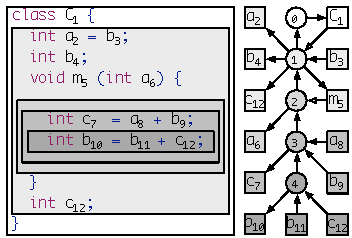
\includegraphics{figures/scope-graphs/subsequent/vars.pdf}
\end{boxedminipage}
\vspace*{-\baselineskip}
\caption{Subsequent scoping of Java variables modeled by nested scopes.}
\figurelabel{java:vars}
\end{wrapfigure}

Our scopes are sets of mutually recursive declarations. This makes it easy to
model a construct such as \pcfmcode{letrec} as we have seen in \Section{coverage}.
However, the scope constructs in many languages have a `definition before use'
policy in which bindings are only visible to references appearing `later' in the
program.
% (\TODO{speculate on the origin of such policies; Such a policy is a natural
% result of one-pass compilers.}) 
For example, the variable declarations in a
block in C or Java are only visible to the subsequent statements in the block.
While colloquially such a block is thought of as a single scope, in fact each
variable declaration opens a new scope, much like the bindings in the sequential
let construct.
\Figure{java:vars} shows how the policy is encoded for blocks in Java by placing
each declaration in a new scope that dominates the references in subsequent
statements.

% For example, in ML, the declaration of a variable with a def \TODO{notation?} is
% only visible \emph{after} in the remainder of the scope in which it is declared

%\paragraph{subsequent scope}
%
% notes about name binding rules in Java (?)
%
% The scope of a formal parameter of a method, constructor, or lambda expression is 
%   the entire body of the method, constructor, or lambda expression.
% 
% The scope of a local variable declaration in a block is the rest of the block in which the declaration appears, 
%   starting with its own initializer and including any further declarators to the right in the local variable declaration statement.
% 
% The scope of a local variable declared in the ForInit part of a basic for statement 
%   includes all of the following:
%   Its own initializer
%   Any further declarators to the right in the ForInit part of the for statement
%   The Expression and ForUpdate parts of the for statement
%  The contained Statement
% 
% The scope of a local variable declared in the FormalParameter part of an enhanced for statement is 
%   the contained Statement.
% 
% A declaration $d$ of a local variable named $n$ shadows, throughout the scope of $d$, 
%   the declarations of any other fields named $n$ that are in scope at the point where $d$ occurs, and 
%   the declarations of any other variables named $n$ that are in scope at the point where $d$ occurs but are not declared in the innermost class in which $d$ is declared.
% 
% It is a compile-time error if the name of a formal parameter is used to 
%   declare a new variable within the body of the method, constructor, or lambda expression, 
%   unless the new variable is declared within a class declaration contained by the method, constructor, or lambda expression.
% 
% It is a compile-time error if the name of a local variable $v$ is used to 
%   declare a new variable within the scope of v, 
%   unless the new variable is declared within a class whose declaration is within the scope of $v$.




% \paragraph{Field Access Modifiers in Java.}
% 
% \TODO{Don't understand this paragraph at all, really.}
% The previous example is imprecise, since it does not consider field access modifiers.
% This keeps \javacode{private} and \javacode{protected} fields visible,
%   yielding additional resolutions.
% From an IDE perspective, these resolutions are valuable, since they hint to
%   possible resolutions, when access modifiers are changed.
% Erroneous resolutions to \javacode{private} fields can be filtered by a language-specific well-formedness predicate,
%   which rejects resolution paths using imports of class scopes.
% Erroneous resolutions to \javacode{protected} requires a more sophisticated well-formedness predicate,
%   which considers the package scope of both class declarations. 

% The scope of a declaration of a member $m$ declared in or inherited by a class
% type $C$ is the entire body of $C$, including any nested type declarations.
% 
% A declaration $d$ of a field named $n$ shadows, throughout the scope of $d$, the
% declarations of any other variables named $n$ that are in scope at the point
% where $d$ occurs.

\subsection{Compilation Units and Packages in Java}

Scopes do not always correspond to single, continuous program fragments.
For example, in Java~\cite{JLS8}, 
  the scope of a top-level type name is all type declarations in the package in which it is declared.
Those type declarations can be spread over multiple, discontinuous program fragments,
  since a package can consist of a number of compilation units.

A compilation unit can be modeled as a scope,
  which imports other scopes associated with the same package name.
For example, 
  \Figure{java:units} shows two compilation units contributing to the same package \javacode{p}.
Each compilation unit declares package \javacode{p} in the root scope
  and associates the declaration with a scope for top-level type declarations.
Types \javacode{C} and \javacode{D} are declared in separate scopes, 
  but are reachable in both scopes via imports from scopes associated with \javacode{p}.
This approach follows the Java terminology, where each compilation unit declares its package.

\begin{figure}[t]
\begin{minipage}{0.42\textwidth}
\begin{boxedminipage}{\hsize}
\centering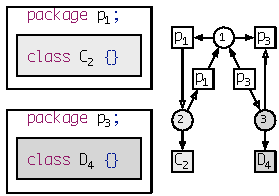
\includegraphics{figures/scope-graphs/java/units.pdf}
\end{boxedminipage}
\caption{Java compilation units modeled by import edges.}
\figurelabel{java:units}
\end{minipage}
\hfill
\begin{minipage}{0.56\textwidth}
\begin{boxedminipage}{\hsize}
\centering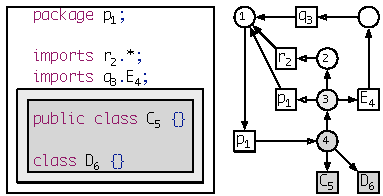
\includegraphics{figures/scope-graphs/java/imports.pdf}
\end{boxedminipage}
\caption{Java import declarations modeled by nested lexical scopes.}
\figurelabel{java:imports}
\end{minipage}
\end{figure}

\paragraph{Import Declarations.}

\Figure{java:imports} shows a compilation unit with two import declarations.
Java supports two kinds of type-import declarations in compilation units.
A \emph{single-type-import declaration} 
  imports a single type.
A \emph{type-import-on-demand declaration} 
  allows all accessible types of a package or type to be imported as needed. 
Thereby, types imported by single-import declarations shadow 
  types of the same name imported by import-on-demand declarations, 
  as well as top-level types of the same name declared in other compilation units of the same package.
The scope of an imported type name is all type declarations in the compilation unit in which the import declaration appears.

We model visibility of imported declarations by three lexical scopes per compilation unit.
The first scope handles all import-on-demand declarations.
The second scope 
  imports type declarations from other compilation units of the same package,
  and declares aliases for single-type-import declarations.
Those aliases act as a declaration and as a reference to the imported name.
According to the default visibility policy, 
  the alias declarations shadow imported declarations from the second and first scopes.
The third scope is associated with the package name and 
  declares the types of the compilation unit.
Those local declarations shadow declarations from other compilation units or packages.

\paragraph{Example.}

The scope graph diagram in \Figure{java:imports} shows 
  a root scope for package names and three lexical scopes for the compilation unit.
Scope $2$ imports from a package \javacode{r}
  and scope $3$ imports from other compilation units from package \javacode{p}.
The single-import declaration \javacode{q.E} is modeled as a qualified name resolution in the global scope
  and as a declaration in scope $3$.
Scope $4$ declares the top-level types \javacode{C} and \javacode{D}.

\paragraph{Accessibility.}

In Java, the reachability of type declarations can be influenced by access modifiers.
In the example, \javacode{C} and \javacode{D} can be accessed in other compilation units of \javacode{p},
  but \javacode{D} cannot be accessed in other packages.
To model accessibility, we need to distinguish 
  \javacode{public}  from \emph{package-private} classes, and
  imports of compilation units of the same package from regular imports in the scope graph.
We can then define a Java-specific well-formedness predicate which rejects
  paths with regular imports of package-private classes.

\subsection{Namespaces and Partial Classes in C\#}

While Java packages can be declared in multiple compilation units,
  C\# namespaces are open-ended,
  allowing also for multiple declarations of a namespace in the same compilation unit.
In a similar way, C\# supports open-ended class declarations.
\Figure{csharp:partial} shows two declarations of namespace \javacode{N}, 
  both partially declaring a class \javacode{C}.
The left part declares a field \javacode{f},
  while the right part is referring to this field.
Similar to Java import declarations, 
  the using directive in the left part only affects the left namespace declaration. 
  
We can model those partial scopes similarly to packages in Java.
Each namespace declaration corresponds to two lexical scopes,
  where local declarations in the second scope hide imported declarations in the first scope.
The second scope also imports from other namespace declarations for the same namespace.
The same pattern can be applied for partial class declarations.
However, C\# supports proper nesting of namespaces and partially qualified names.
Thus, we can no longer resolve to other partial declarations of the same name in global scope.
With the default reachability policy,
  we might find other partial declarations for the same name in lexical scope.
Instead, we need to make sure to resolve only to parts in the same surrounding namespace 
  (which might again be declared in several parts).
This can be achieved by distinguishing imports of parts from regular imports,
  and a reachability policy for the former, which rejects parent paths. 

\begin{figure}[t]
\begin{boxedminipage}{\hsize}
\centering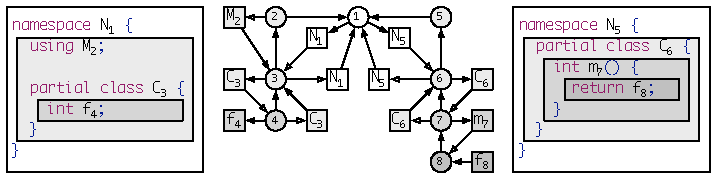
\includegraphics{figures/scope-graphs/csharp/partial.pdf}
\end{boxedminipage}
\caption{C\# namespaces and partial classes modeled by import edges.}
\figurelabel{csharp:partial}
\end{figure}

%%%%%%%%%%%%%%%%%%%%%%%%%%%%%%%%%%%%%%%%%%%%%%%%%%%%%%%%%
\endinput
  %\usepackage{graphics} is needed for \includegraphics
\begin{figure}[h]
\begin{minipage}{3cm}
\begin{lstlisting}[language=Java]
val x = 1;
{ 
  import p.x;
  x // ambiguous reference
}
\end{lstlisting}
\end{minipage}
  \caption{Java package and type declarations in different compilation units.}
  \label{figureLabel}
\end{figure}





%\subsection{PCFM}
	  
		systematic discussion of typical examples and corner cases
		
		collect all the examples in this section 
		
		
%\subsection{Namespaces.}

Some programming languages distinghuish different kinds of names. A reference of
one kind cannot refer to a declaration of another kind of name.
For example, in Java, classes, class variables, and methods are distinct kinds
of names, which do not interfere.
In ML, variables and algebraic datatype constructors are distinguished
syntactically by requiring that constructors start with a capital and variables
with a lower case letter. 
In the NaBL name binding DSL this notion is
characterized using the concept of \emph{namespaces} \cite{KonatKWV12}.

In this paper, we do not explicitly consider the notion of namespaces,
effectively assuming a single namespace.
However, this is not a limitation, since namespaces can be encoded by mapping a
name in a program to a pair of its namespace and the name. For example, we can
distinghuish a variable with name $x$ from a method with name $x$ by encoding
them as $(V, x)$ and $(M, x)$, respectively.
\GW{
  It is a limitation for references, since it requires to know the namespace before resolution. 
  Java's ambiguous names cannot be modeled this way.
}
\GW{
  Obscuring is another interesting topic here. Can we handle this by (language-specific) disambiguation?
  \emph{
    A simple name may occur in contexts where it may potentially be interpreted as the name of a variable, a type, or a package. 
    In these situations, the rules of §6.5 specify that a variable will be chosen in preference to a type, and that a type will be chosen in preference to a package. 
    Thus, it is may sometimes be impossible to refer to a visible type or package declaration via its simple name.
  }
}
\EV{Perhaps this discussion is somewhat distracting and not relevant for the
flow of the story at this position anyway and could be moved to a later point in
the paper, such as the extensions section 4.}

%\subsection{Multiple source files.}

Programs are typically distributed over multiple source files and name binding
crosses file boundaries.
Scopes do not need to correspond to nodes in an
AST, but can represent virtual code units such as a project or library.
The scope graphs for the ASTs of the individual files are joined under a common
scope.

	\newpage
	\section{Proofs}
\label{app:proofs}

We often write just $\r{x}$ (resp. $\d{x}$) for a reference (resp. declaration) at some particular but unnamed position.

%\renewcommand{\scopea}[1]{\stackrel{#1}{\longrightarrow}}
\renewcommand{\labelenumi}{\tab $\roman{enumi})$ }

\subsection{Termination of resolution algorithm}\label{subsection:inlinedresalg}

Figure \ref{fig:inlinedresalg} presents the inlined resolution algorithm that only use strictly 
decreasing recursive calls.

\begin{figure}[h]
\renewcommand{\S}{\mathcal{S}}
\begin{boxedminipage}{\hsize}
$
\begin{array}{ll}
  \Res{\seeni}{\r{x}} & := \left\{ \di{x}{i} \left| \exists S\ s.t.\ \r{x} \in \R{S} \wedge \di{x}{i} \in 
  \left(\begin{array}{l}
    \Env{D}{\{\r{x}\} \cup \seeni}{\emptyset}{S}  \\
     \triangleleft ~\Env{I}{\{\r{x}\} \cup \seeni}{\emptyset}{S}  \\
     \triangleleft ~\Env{P}{\{\r{x}\} \cup \seeni}{\emptyset}{S}    
  \end{array}\right)
 \right\}\right. \smallskip  \\
\Env{D}{\seeni}{\seens}{S} &:= \left\{
    \begin{array}{l}
      \emptyset  \text{ if } S\in\seens\\
      \D{S}\smallskip\\
    \end{array}
 \right.\smallskip\\
 \Env{I}{\seeni}{\seens}{S} &:= \left\{
    \begin{array}{l}
      \emptyset  \text{ if } S\in\seens\\
      \bigcup \left\{
        \begin{array}{l}
          \Env{D}{\seeni}{\{S\}\cup\seens}{S_y}\\
          \triangleleft ~\Env{I}{\seeni}{\{S\}\cup\seens}{S_y}
        \end{array}\hspace*{-1mm}
      \left| 
        \begin{array}{l}
          \r{y} \in \I{S} \setminus \seeni\ \wedge \\
          \exists S_y\ s.t.\ \r{y} \in \R{S_y}\ \wedge \\
          \ds{y}{S_y} \in 
          \left(\begin{array}{l}
              \Env{D}{\{\r{x}\} \cup \seeni}{\emptyset}{S_y}  \\
              \triangleleft ~\Env{I}{\{\r{x}\} \cup \seeni}{\emptyset}{S_y}  \\
              \triangleleft ~\Env{P}{\{\r{x}\} \cup \seeni}{\emptyset}{S_y}    
            \end{array}\right)
        \end{array}\hspace*{-1.5mm}
      \right\}\right.\smallskip\\
    \end{array}
 \right.\smallskip\\
 \Env{P}{\seeni}{\seens}{S} & := \left\{
   \begin{array}{l}
     \emptyset  \text{ if } S\in\seens\\
     \left(\begin{array}{l}
       \Env{D}{\seeni}{\{S\}\cup\seens}{\P{S}} \\
       \triangleleft ~\Env{I}{\seeni}{\{S\}\cup\seens}{\P{S}} \\
       \triangleleft ~\Env{P}{\seeni}{\{S\}\cup\seens}{\P{S}} 
     \end{array}\right)
   \end{array}
 \right. \smallskip\\
\end{array}\medskip
$
\end{boxedminipage}
\caption{Inlined resolution algorithm}
\label{fig:inlinedresalg}
\end{figure}

\subsection{Well-formed Paths and Specificity Ordering}

We can give a simple grammatical characterization of well-formed paths, and
use it to define a measure on paths that is compatible with the specificity 
ordering.

\begin{lemma}[Well-formed path measure]\label{lem:wfpm} For all well-formed paths $p$, there
exist $i,j \geq 0$ such that $p = \pstep^i \cdot \istep{\_}{\_}^j$. 
We write
$m(p)$ for the corresponding pair $(i,j)$ and write $<$ for the lexicographic ordering
on these pairs.
\end{lemma}

\begin{lemma}[WF path measure and specificity ordering are compatible]\label{lem:pathmescomp} 
For all well-formed paths $p,p'$,
\begin{equation*}
 p\cdot\dstep{\_} < p'\cdot\dstep{\_} \iff m(p) < m(p')  
\end{equation*}
\end{lemma}
\begin{proof} Let $m(p) = (i,j)$ and $m(p') = (i',j')$. Let
$q = p\cdot\dstep{\_}$ and $q' = p'\cdot\dstep{\_}$,
and write $q_k,q'_{k}$ for the $k$-th steps of $q$ and $q'$, respectively.
\\ ($\Longrightarrow$) Assume $p < p'$.
Then in the first step $k$ where $q$ and $q'$ differ (i.e., the first application of rule $Lex1$),
we have three possible cases:
\begin{itemize}
 \item ($DI$) $q_k = \dstep{\_}$ and $q'_k = \istep{\_}{\_}$: then $i = i'$ and $j < j'$; hence $m(p) < m(p')$.
 \item ($IP$) $q_k = \istep{\_}{\_}$ and $q'_k = \pstep$: then $i < k \le i'$; hence $m(p) < m(p')$.
 \item ($DP$) $q_k = \dstep{\_}$ and $q'_k = \pstep$: then $i < k \le i'$; hence $m(p) < m(p')$. 
\end{itemize}
($\Longleftarrow$) Suppose $m(p) < m(p')$. Then there are two cases:
\begin{itemize}
 \item $i < i'$: then $\forall k \leq i, q_k = q'_k$,  
                    $q_{i+1} = \istep{\_}{\_}$ or $\dstep{\_}$, and $q'_{i+1} = \pstep$; hence $p < p'$.
 \item $i = i'$ and $j < j'$: then  $\forall k \leq i+j, q_k = q'_k$,
                    $q_{i+j+1} = \dstep{\_}$ and $q'_{i+j+1} = \istep{\_}{\_}$; hence $p < p'$.
\end{itemize}
 \qed
\end{proof}


\subsection{Cycles in Resolution Paths}

To enforce the termination of the resolution algorithm, we only look for cycle-free paths in this algorithm.
Looking for cycle-free paths is sufficient:

\begin{definition}[Cycle] 
\label{def:cycle}
A path $p$ contains a cycle if there exist $p_1, p_2, p_3$ 
such that $p = p_1 \cdot p_2 \cdot p_3$, $p_2 \neq []$, and 
there exist $A$, $B$ and $S$ such that 
$\seeni \vdash p_1 : A \medge S$, $\seeni \vdash p_2 : S \medge S$,and
$\seeni \vdash p_3: S \medge B$.
\end{definition}

\begin{lemma}[Lemma~\ref{lemma:cycle-free}: Resolution paths are cycle-free.]
If 
\begin{equation*}
\seeni \vdash p : \r{x} \resolve \d{x}
\end{equation*}
then $p$ is cycle-free.
\end{lemma}
\begin{proof}
By rule $(X)$, we have $\seeni' \vdash p: S_r \resolve \d{x}$ where
$\seeni'$ = $\{\r{x}\} \cup \seeni$ and
$S_r$ is the (unique) scope such that $\r{x} \in \R{S_r}$.
By rule $(V)$ we have $\seeni' \vdash p: S_r \reach \d{x}$ and
\begin{equation}\label{eqn:noshorter}\tag{\mbox{$*$}}
\nexists\ p'\ \di{x}{i'}\ s.t.\ \seeni' \vdash p': S_r \reach \di{x}{i'}\ \mbox{\it and}\ p' < p.
\end{equation}
By rule $(R)$ we have 
$\seeni' \vdash p_0: S_r \medge S_d$ where $p = p_0 \cdot \dstep{\d{x}}$ and
$S_d$ is the (unique) scope such that $\d{x} \in \D{S_d}$;
moreover, $\WF(p_0)$ holds, so by Lemma~\ref{lem:wfpm}, 
$p_0=\pstep^i\cdot\istep{\_}{\_}^j$ for some $i,j \geq 0$.
We claim $p_0$ contains no cycle.
For suppose it does, with $p_1, p_2, p_3$ and $S$ as in Definition~\ref{def:cycle}, 
and consider the {\it shrunken} path $p' = p_1 \cdot p_3$. Then, since
$\seeni' \vdash p_1 : S_r \medge S$ and $\seeni' \vdash p_3 : S \medge S_d$, we have
$\seeni' \vdash p' : S_r \medge S_d$.  Also, $p'$ must have the form $\pstep^{i'}\cdot\istep{\_}{\_}^{j'}$,
where, depending on the position of $p_2$ in $p_0$,  
either (i) $i' < i$ or (ii) $i' = i$ and $j' < j$. Therefore $\WF(p')$ holds, 
and we have $\seeni' \vdash p' \cdot \dstep{\d{x}} : S_r \reach \d{x}$.
But since $m(p') = (i',j') < (i,j) = m(p_0)$, then by Lemma~\ref{lem:pathmescomp}, $p'\cdot\dstep{\d{x}} < p_0\cdot\dstep{\d{x}}$, contradicting ($\ref{eqn:noshorter}$). 
So $p_0$ has no cycle, and hence neither does $p$. \qed
\end{proof}

\begin{comment}

\begin{lemma}[Cycle-free Path Existence]
\label{lemma:cycle-free} 
If there is a path for a resolution then there is
a cycle-free path for this resolution.
\vspace*{-.6\baselineskip}
$$
 \forall\seeni,\r{x},\d{x},  (\exists p\ s.t.\ \seeni \vdash p : \r{x} \resolve \d{x}) \Longrightarrow 
(\exists p, p\ \mbox{\it is cycle-free} \wedge \seeni \vdash p : \r{x} \resolve
\d{x}) $$
\end{lemma}
\begin{proof}
The set of all resolution paths 
$\{ p \mid \seeni \vdash p\cdot\dstep{\d{x}} : \r{x} \resolve \d{x}\}$
must contain (at least one) shortest path $p$ (we use \emph{shorter} when referring to  the length of the path and \emph{smaller} when referring to the path ordering $<$).  
We claim $p$ contains no cycle.
For suppose it does, with $p_1, p_2, p_3$ as in Definition~\ref{def:cycle} and 
consider the {\it shrunken} path $p' = p_1 \cdot p_3$. Then:
\begin{equation*}
\r{x} \in S_r \wedge \d{x} \in S_d \wedge \seeni \vdash p' : S_r \medge S_d
\end{equation*}
Moreover, by considering all possible patterns of steps for $p_2$, 
we can see that $p'$ is well-formed. Hence
\begin{equation*}
\seeni \vdash p' : S_r \reach \d{x}  
\end{equation*}
We claim $p'$ is also a minimal (most-specific) path resolving $\r{x}$ under $\seeni$.
For suppose not. Then there is a $q$ such that:
\begin{equation*}
  \seeni \vdash q : \r{x} \reach \d{x} \wedge q < p_1 \cdot p_3 
\end{equation*}
Then we have two cases:
  \begin{itemize}
   \item $q= q_1 \cdot q_2 $ and $q_1 < p_1$; and therefore $q < p_1\cdot p_2 \cdot p_3 = p$   
   \item $q = p_1 \cdot q_2 $ and $q_2 < p_3$; in this case $p_1 \cdot p_2
   \cdot q_2$ is also a well-formed path more specific than $p_1\cdot p_2 \cdot p_3 = p$,
  \end{itemize}
In either case, we have exhibited a well-formed path more specific than $p$, contradicting
the assumed minimality of $p$. 
Therefore  $p'$ is indeed minimal, so we have:
\begin{equation*}
\seeni \vdash p' : \r{x} \resolve \d{x} 
\end{equation*}
But $p'$ is strictly shorter than $p$, which is a contradiction. 
So $p$ must not contain a cycle. \qed
\end{proof}
\end{comment}

\subsection{Shadowing and Resolution}

%We present here a lemma that allows us to exhibit a minimal (i.e., most specific) path for the resolution of a reference
%as soon as we know that some declaration is reachable from the reference. 
%In proofs of minimality of $p$, it will allow us not only to suppose (for contradiction) that
%$p$ is not minimal (therefore there is more specific path $p'$ such that $\seeni,\seens \vdash p' : S \reach \d{x}$) 
%but that there is a more specific path $p'$ such that $\seeni,\seens \vdash p' : S \resolve \d{x}$.
%Using this measure we can directly prove the existence of a minimal well-formed resolution path 
%when a well-formed resolution path exists. This means that as soon as a declaration is reachable from a reference, it can only be shadowed
%by other declarations and that this shadowing process stops somewhere. 
%APT: I couldn't find a way to clarify this paragraph to my satisfaction...


\begin{lemma}[Shadowing preserves resolution] \label{lemma:shadowexists}
If there is a reachability path from a scope to the declaration of a variable, then there
is a visibility path, at least as specific, from that scope to some declaration of 
that variable.
\begin{multline*}
\forall\ \seeni\ \seens\ S\ p\ \di{x}{i},
\seeni,\seens \vdash p : S \reach \di{x}{i} \Longrightarrow\\
(\exists\ q\ j\ s.t.\ \seeni,\seens \vdash q : S \resolve \di{x}{j} \wedge q \leq p).
\end{multline*}
\end{lemma}
\begin{proof} Fix $\seeni$, $\seens$, $S$, $p$, and $\di{x}{i}$. Let 
$W := \{ p' \mid \exists i'\ s.t.\ \seeni,\seens \vdash p' : S \reach \di{x}{i'} \wedge p' \le p\}$
be the set of reachability paths from $S$ to $x$ that are at least as specific as $p$. 
We need to show that $W$ contains a minimal reachable path, i.e., an element $q$ such that:
$\forall i'\ p', \seeni,\seens \vdash p' : S \reach \di{x}{i'} \Rightarrow \neg (p' < q)$.
$W$ is not empty (it contains $p$) and the set of associated measures of 
its members, i.e.
\begin{equation*}
 m(W) = \{ m(p') \mid \exists\ i'\ s.t.\ \seeni \vdash\ p'\cdot\dstep{\di{x}{i'}} : S \reach \di{x}{i'} \wedge p'\cdot\dstep{\di{x}{i'}} \le p\}
\end{equation*}
is a set of pairs of natural
numbers, on which the lexicographic ordering is well-founded. Thus it
has at least one smallest element, with associated path $q$ and declaration position $j$, 
and using lemma \ref{lem:pathmescomp}, $q$ is minimal for $<$ in $W$. 
We claim that $q$ is minimal among all reachable paths.
For suppose not; then there is a path $q' < q$ and an $i'$ such that  
\begin{equation*}
  \seeni,\seens \vdash\ q' : S \reach \di{x}{i'}. 
\end{equation*}
But since $q$ is in $W$ then $q \leq p$ and $<$ is transitive so $q' < p$ and then $q' \in W$,
contradicting the minimality of $q$ in $W$.
Therefore we have an element $q$ and position $j$ such that:
\begin{equation*}
  \seeni,\seens \vdash\ q : S \resolve \di{x}{j} \wedge q \le p 
\end{equation*}\qed
\end{proof}

\subsection{Correctness of resolution algorithm}

% \begin{lemma} \label{lemma:weakening}
%   $\forall\ \seeni\ \seens\ p\ S\ S'\ S''\ s.t. \seeni,\{S\}\cup\seens \vdash p  : S' \medge S'' \longrightarrow
%   \seeni,\seens \vdash p : S' \medge S''$  
% \end{lemma}
% \begin{proof}
%   Trivial, by induction on p, $B \notin \{S\}\cup\seens \Rightarrow B \notin \seens$. 
% \end{proof}

We now proceed to prove the correctness of the resolution algorithm. We first address some auxiliary lemmas that we will need in the proof.
First, the path uniquely encodes the sequence of scopes in the resolution: 
\begin{lemma}[Transition unique] \label{lemma:transuniq}
\begin{equation*}
\seeni,\seens \vdash s : S \edge S_1 \Longrightarrow \seeni,\seens \vdash s : S \edge S_2 \Longrightarrow S_1 = S_2
\end{equation*}
\end{lemma}
\begin{proof} Trivial by case analysis on $s$: import steps record the imported scope $S_y$ to which they step,
and parent steps go to the uniquely defined parent.\qed
\end{proof}

Then we state that we can cut a resolution path for the reachability relation, i.e., if a declaration is reachable from a scope $S$ then it is also reachable from any scope appearing in the resolution.

\begin{lemma}[Reachable tail] \label{lemma:tailreach} If a definition is reachable from a scope $S$ through scope $S'$ then it is also reachable from $S'$:\\
  \begin{equation*}
   \forall\ \seeni\ \seens\ s\ p\ S\ d,
    \begin{array}[t]{rl}
    \seeni,\{S\}\cup\seens & \vdash s : S \edge S' \Longrightarrow \\  
    \seeni,\seens & \vdash s \cdot p\cdot\dstep{\d{x}} : S \reach \d{x} \Longrightarrow \\
    & \seeni,\{S\}\cup\seens \vdash p\cdot\dstep{\d{x}} : S' \reach \d{x}    
    \end{array} 
  \end{equation*}
   
\end{lemma}
\begin{proof} If $s\cdot p$ is well formed then $p$ is also well formed. By inversion of:
  \begin{equation*}
    \seeni,\seens \vdash s \cdot p \cdot \dstep{\d{x}} : S \reach \d{x} 
  \end{equation*}
and using lemma \ref{lemma:transuniq}, we get:
\begin{enumerate}[leftmargin=15mm]
 \item $\seeni,\{S,S'\}\cup\seens \vdash p : S' \medge S_d $
 \item $S \notin \seens$
 \item $S' \notin \seens$
 \item $\d{x} \in \D{S_d}$
\end{enumerate}
Therefore, using $i)$, $iii)$ and $iv)$, we get by rule $(R')$:
\begin{equation*}
\seeni,\{S\}\cup\seens \vdash p\cdot\dstep{\d{x}} : S' \reach \d{x}   
\end{equation*}\qed
\end{proof}

Similarly, if a declaration is visible from a reference then it is visible all along the path.

\begin{lemma}[Visible tail] \label{lemma:tailres}
If a definition is visible from a scope $S$ through scope $S'$ then it is also visible from $S'$:\\
\begin{equation*}
\forall\ \seeni\ \seens\ s\ p\ S\ \di{x}{i}, 
\begin{array}[t]{rll}
\seeni,\{S\}\cup\seens & \vdash s : S \edge S' \Longrightarrow & (i) \\
\seeni,\seens & \vdash s \cdot p \cdot \dstep{\di{x}{i}} : S \resolve \di{x}{i} \Longrightarrow & (ii)\\ 
& \seeni,\{S\}\cup\seens \vdash p \cdot \dstep{\di{x}{i}} : S' \resolve \di{x}{i}  
\end{array}
\end{equation*}
\end{lemma}
\begin{proof} By inversion on $(ii)$
we get:
\begin{itemize}[leftmargin=15mm]
 \item[$(*)$\tab] $\seeni,\seens \vdash s \cdot p \cdot \dstep{\di{x}{i}} : S \reach \di{x}{i}$ 
 \item[$(**)$\tab] $\forall\ p'\ \di{x}{i'}\ s.t.\ \seeni,\seens \vdash p' : S \reach \di{x}{i'} \Rightarrow \neg p' < s\cdot p $ 
\end{itemize}
By lemma \ref{lemma:tailreach} and $(*)$ we have:
\begin{itemize}[leftmargin=15mm]
 \item[$(\lozenge)$\tab] $\seeni,\{S\}\cup\seens \vdash p \cdot \dstep{\di{x}{i}} : S' \reach \di{x}{i}$
\end{itemize}
Suppose $p$ is not minimal. Then there is a $p'$ such that:
\begin{itemize}[leftmargin=15mm]
 \item[$(Hr)$\tab] $\seeni,\{S\}\cup\seens \vdash p' \cdot \dstep{\di{x}{i'}} : S' \reach \di{x}{i'}$
 \item[$(<)$\tab] $ p' \cdot \dstep{\di{x}{i'}} < p \cdot \dstep{\di{x}{i}} $
\end{itemize}
If $s = \pstep$ then, since inversion on $(Hr)$ gives us $\WF(p')$, we obtain $\WF(s \cdot p')$.
Alternatively, if $s = \istep{\_}{\_}$ then, since inversion on $(*)$ gives us $\WF(s\cdot p)$, we know $p$
has the form $\istep{\_}{\_}^*$.
Then by (<), we must have that $p'$ also has the form $\istep{\_}{\_}^*$, so we again obtain $\WF(s \cdot p')$.
Therefore, by inversion of $(Hr)$ and using $(i)$ we have: \\
\begin{equation*}
\seeni,\seens \vdash s\cdot p'\cdot\dstep{\di{x}{i'}} : S \reach \di{x}{i'}  
\end{equation*}
which contradicts $(**)$.
Therefore $p$ is minimal and using $(\lozenge)$ we have:
\begin{equation*}
\seeni,\{S\}\cup\seens \vdash p \cdot \dstep{\di{x}{i}} : S' \resolve \di{x}{i}.
\end{equation*}\qed
\end{proof}

%To shorten notation, we write $\pathx{C}$ for $\paths{C}{\seeni}{\seens}{S}$ for each clause class $C$.
The elements in the $\pathx{C}$ sets are incomparable under the specificity ordering.

\begin{lemma}[Path set minima]\label{lemma:notinf}
\begin{equation*}
\forall\ C\ \seeni\ \seens\ S,\ \forall p, p' \in \paths{C}{\seeni}{\seens}{S},\ \neg p < p'.
\end{equation*}
\end{lemma}
\begin{proof} Assume for contradiction that $p < p' (*)$. Proceed by case analysis on $C$:
  \begin{itemize}
   \item Case $I$: by definition of $\pathx{I}$:
    \begin{enumerate}[leftmargin=15mm]
     \item $p = \istep{\r{y}}{\ds{y}{S_y}}\cdot \bar{p}$ 
     \item $p' = \istep{\r{z}}{\ds{z}{S_z}}\cdot \bar{p}'$
     \item $\seeni,\{S\}\cup\seens \vdash \bar{p} : S_y \resolve \di{x}{i} $
     \item $\seeni,\{S\}\cup\seens \vdash \bar{p}' : S_z \resolve \di{x}{i'} $
    \end{enumerate}
    By inversion of $(*)$, $\istep{\r{y}}{\ds{y}{S_y}} = \istep{\r{z}}{\ds{z}{S_z}}$ and hence $S_y = S_z$, so we cannot have $\bar{p} < \bar{p'}$ since both $\bar{p}$ and $\bar{p}'$ are minimal.
    \item Case $P$: Proof is similar to case $I$: both $\bar{p}$ and $\bar{p}'$ are resolutions from $\P{S}$.
    \item Cases $L,V,D$: trivial.\qed
  \end{itemize}
\end{proof}


\newcommand{\Case}[1]{\textbf{Case #1}:}
\renewcommand{\theenumi}{\arabic{enumi}}
\renewcommand{\labelenumi}{\theenumi)}


We now proceed to prove that the different functions of the algorithm compute definitions corresponding to paths in the $\pathx{C}$ sets.
\begin{lemma}
[Lemma~\ref{lemma:pathset-alg}]
For each class $C \in \{V,L,D,I,P\}$: 
\begin{equation*}
\forall\ \seeni\ \seens\ S, \Env{c}{\seeni}{\seens}{S} = \defsof{\paths{C}{\seeni}{\seens}{S}}
\end{equation*}
\end{lemma}
\begin{proof}
The proof is by three nested inductions,
the outer one on $\seeni$ (or, more strictly, on the size of \mbox{$|\R{\G} \setminus \seeni|$}, the references
\emph{not} in $\seeni$) and the second one on $\seens$ (more strictly, the size of \mbox{$|\S{\G} \setminus \seens|$}, 
the scopes \emph{not} in $\seens$) and the third one on the class $C$, with the order $V > L > D,I,P$.
We then pick an $\d{x}$, and proceed according to the class $C$:\smallskip

\noindent \Case{D} \\
$\d{x} \in \Env{D}{\seeni}{\seens}{S} \iff$ (by definition of $\Envu{D}$) \\
$\d{x} \in \D{S} \wedge S \not\in \seens \iff$ (by rule $(R')$)\\
$\seeni,\seens\vdash \dstep{\d{x}} : S \reach \d{x} \iff$ (by definition of $\Delta$ and $\pathx{D}$)\\
$\d{x} \in \defsof{\paths{D}{\seeni}{\seens}{S}}$\\

\noindent \Case{P}\\
$\d{x} \in \Env{P}{\seeni}{\seens}{S} \iff$ (by definition of $\Envu{P}$) \\
$\d{x} \in \Env{V}{\seeni}{\{S\} \cup \seens}{\P{S}} \wedge S \not\in \seens \iff$ (by induction on $\seens$)\\
$\d{x} \in \defsof{\paths{V}{\seeni}{\{S\} \cup \seens}{\P{S}}} \wedge S \not\in \seens \iff$ (by definition of $\Delta$, $\pathx{V}$)\\
% really need an additional little lemma here 
$\exists p\ s.t.\ \seeni,\{S\}\cup\seens \vdash p \cdot \dstep{\d{x}} : \P{S} \resolve \d{x} \wedge S \notin \seens$\\ 
\tab $\iff$ ($\Longrightarrow$ by rule $(P)$  and rules $(V',R')$; $\Longleftarrow$ by weakening)\\
$\exists p\ s.t.\ \seeni,\{S\}\cup\seens \vdash p \cdot \dstep{\d{x}} : \P{S} \resolve \d{x} \wedge S \notin \seens \wedge \\
\tab\tab\tab\seeni \vdash \pstep : S \edge \P{S} \wedge \P{S} \notin \{S\}\cup \seens$\\ 
\tab $\iff$ (by rules $(R')$ and $(T')$)\\
$\exists p\ s.t.\ \seeni,\{S\}\cup\seens \vdash p \cdot \dstep{\d{x}} : \P{S} \resolve \d{x} \wedge \seeni,\seens \vdash \pstep\cdot p\cdot \dstep{\d{x}} : S \reach \d{x}$ \\
\tab$ \iff$ (by definition of $\Delta$ and$\pathx{P}$)\\
% and again here
$ \d{x} \in \defsof{\paths{P}{\seeni}{\seens}{S}}$\\

\newcommand{\ttab}{\tab\tab\tab}
\noindent \Case{I}\\
$\d{x} \in \Env{I}{\seeni}{\seens}{S} \iff$ (definition of $\Envu{I}$) \\
$\d{x} \in \bigcup \left\{ \Env{L}{\seeni}{\{S\}\cup\seens}{S_y} \mid \r{y} \in \I{S}\setminus \seeni \wedge \ds{y}{S_y} \in \Res{\seeni}{\r{y}}\right\} \wedge S \not\in \seens$\\
\tab $ \iff$ (by unfolding of $\Res{\seeni}{\r{y}}$ and induction on $\seeni$) \\
$\d{x} \in \bigcup \left\{ \Env{L}{\seeni}{\{S\}\cup\seens}{S_y} \left| 
  \begin{array}{l}
    \r{y} \in \I{S}\setminus \seeni  \wedge\\
    \exists S', \r{y} \in \R{S'} \wedge\\
    \tab \ds{y}{S_y} \in \defsof{\paths{V}{\{\r{y}\}\cup\seeni}{\emptyset}{S'}} 
  \end{array}\right\}\right. \wedge S \not\in \seens$\\
\tab $\iff$ (by definition of $\pathx{V}$ and rule $(X')$)\\
$\d{x} \in \bigcup \left\{ \Env{L}{\seeni}{\{S\}\cup\seens}{S_y} \left|  
  \begin{array}{l}
   \r{y} \in \I{S}\setminus\seeni \wedge \\
   \exists q\ \ds{y}{S_y}\ s.t.\ \seeni \vdash q: \r{y} \resolve \ds{y}{S_y}
\end{array}\right\}\right. \wedge S \not\in \seens$ \\
\tab $\iff$ (by $L$ case of induction on $\seens$) \\
$\exists \r{y}\ q\ \ds{y}{S_y}\ p\ s.t.\\
\ttab \r{y} \in \I{S}\setminus\seeni \wedge \seeni \vdash q:\r{y} \resolve \ds{y}{S_y} \wedge\\
\ttab p \cdot D(\d{x}) \in \paths{L}{\seeni}{\{S\}\cup\seens}{S_y} \wedge S \not\in \seens$\\
\tab$\iff$ (by definition of $\pathx{L}$)\\
$\exists \r{y}\ q\ \ds{y}{S_y}\ p\ s.t.\ \r{y} \in \I{S}\setminus\seeni \wedge \\
\ttab \seeni \vdash q:\r{y} \resolve \ds{y}{S_y} \wedge \\
\ttab \seeni,{\{S\}\cup\seens} \vdash p \cdot \dstep{\d{x}} : S_y \resolve \d{x} \wedge \\
\ttab p \in \istep{\_}{\_}^* \wedge\\
\ttab S \not\in \seens$\\
\tab$\iff$ (by rule $(I)$)\\
$\exists \r{y}\ \ds{y}{S_y}\ p,\\ 
\ttab \seeni \vdash \istep{\r{y}}{\ds{y}{S_y}} : S \edge S_y\\
\ttab \seeni,{\{S\}\cup\seens} \vdash p \cdot \dstep{\d{x}} : S_y \resolve \d{x} \wedge \\
\ttab p \in \istep{\_}{\_}^* \wedge\\
\ttab S \not\in \seens$\\
\tab $\iff$ ($\Longrightarrow$ by $(R')$; $\Longleftarrow$ by weakening)\\
$\exists\ S_x\ \r{y}\ \ds{y}{S_y}\ p,\\ 
\ttab \seeni \vdash \istep{\r{y}}{\ds{y}{S_y}} : S \edge S_y\\
\ttab S_y \notin {\{S\}\cup\seens}\\
\ttab \seeni,{\{S,S_y\}\cup\seens} \vdash p  : S_y \medge S_x\\
\ttab \d{x} \in S_x \wedge\\
\ttab \seeni,{\{S\}\cup\seens} \vdash p \cdot \dstep{\d{x}} : S_y \resolve \d{x} \wedge \\
\ttab p \in \istep{\_}{\_}^* \wedge\\
\ttab S \not\in \seens$\\
\tab $\iff$ (by $(T')$, $(I)$ and $\WF$ definition)\\
$\exists\ S_x\ \r{y}\ \ds{y}{S_y}\ p,\\ 
\ttab \seeni,{\{S\}\cup\seens} \vdash \istep{\r{y}}{\ds{y}{S_y}}\cdot p : S \medge S_x\\
\ttab \d{x} \in S_x \wedge\\
\ttab \seeni,{\{S\}\cup\seens} \vdash p \cdot \dstep{\d{x}} : S_y \resolve \d{x} \wedge \\
\ttab \WF(\istep{\r{y}}{\ds{y}{S_y}}\cdot p \cdot \dstep{\d{x}}) \wedge\\
\ttab S \not\in \seens$\\
\tab $\iff$ (by $(R')$)\\
$\exists\ \r{y}\ \ds{y}{S_y}\ p,\\ 
\ttab \seeni,{\seens} \vdash \istep{\r{y}}{\ds{y}{S_y}}\cdot p \cdot \dstep{\d{x}}: S \reach \d{x} \wedge\\
\ttab \seeni,{\{S\}\cup\seens} \vdash p \cdot \dstep{\d{x}} : S_y \resolve \d{x} $\\
\tab $\iff$ (by definition of $\pathx{I}$)\\
$\exists\ \r{y}\ \ds{y}{S_y}\ p,\\
\ttab \istep{\r{y}}{\ds{y}{S_y}}\cdot p \cdot \dstep{\d{x}} \in \paths{I}{\seeni}{\seens}{S}$\\
\tab $\iff$ (by definition of $\Delta$)\\
$\d{x} \in \defsof{\paths{I}{\seeni}{\seens}{S}}$\\

\noindent \Case{L} 
We split the two directions:

\Case{L.($\Rightarrow$)} \\
$\d{x} \in \Env{L}{\seeni}{\seens}{S} \Rightarrow$ (by definition of $\Envu{L}$) \\
$\d{x} \in \Env{D}{\seeni}{\seens}{S} \hiding \Env{I}{\seeni}{\seens}{S}$\\
By case on the set $\d{x}$ comes from:
\begin{enumerate}
 \item If $\d{x} \in \Env{D}{\seeni}{\seens}{S}$ \\
 then by the induction on the class (since $D < L$) we get:\\
 $\d{x} \in \defsof{\paths{D}{\seeni}{\seens}{S}} \Rightarrow$ (by definition of $\Delta$ and $\pathx{D}$)\\
 $\seeni,\seens \vdash \dstep{\d{x}} : S \reach \d{x} \Rightarrow$ ($\dstep{\d{x}}$ is always minimal)\\ 
 $\seeni,\seens \vdash \dstep{\d{x}} : S \resolve \d{x} \Rightarrow$ (since $\dstep{\d{x}} \in \istep{\_}{\_}^*\cdot \dstep{\_}$)\\
 $\dstep{\d{x}} \in \paths{L}{\seeni}{\seens}{S}\Rightarrow$ (by definition)
 $\d{x} \in \defsof{\paths{L}{\seeni}{\seens}{S}}$
 \smallskip

\item If $\forall\ i,\ \di{x}{i} \notin \Env{D}{\seeni}{\seens}{S}$ and $\d{x} \in \Env{I}{\seeni}{\seens}{S}$
 then by the induction on class (since $I < L$) we get that:
 $\d{x} \in \defsof{\paths{I}{\seeni}{\seens}{S}}$\\
By definition of $\pathx{I}$ there exist $p\ p'\ \r{y}\ \ds{y}{S'}$, such that $p = \istep{\r{y}}{\ds{y}{S'}}  \cdot p'$ and:
\begin{itemize}[leftmargin=15mm]
 \item[$(*)$] $ \seeni,\seens \vdash p : S \reach \d{x}$
 \item[$(**)$] $ \seeni,\{S\} \cup \seens \vdash p' : S' \resolve \d{x}$
\end{itemize}
From $(*)$ we have $\WF(\istep{\r{y}}{\ds{y}{S'}}  \cdot p')$, which trivially implies that
 $p \in \istep{\_}{\_}^*\cdot \dstep{\_}$.\\
Thus, to prove that $\d{x} \in \defsof{\paths{L}{\seeni}{\seens}{S}}$ it is sufficient to prove that $ \seeni,\seens \vdash p : S \resolve \d{x}$ and given $(*)$ we need only 
prove that $p$ is minimal:\\
Assume for contradiction that there is a path $\bar{p}$ such that:
\begin{itemize}[leftmargin=15mm]
 \item[$ (\diamond)$] $ \seeni,\seens \vdash \bar{p} : S \reach \di{x}{i}$
\end{itemize}
and $\bar{p} < \istep{\r{y}}{\ds{y}{S'}}\cdot p'$. Then we have 2 cases:
\begin{itemize}[leftmargin=10mm]
 \item $\bar{p} = \dstep{\di{x}{i}}$:\\
  then by definition of $\pathx{D}$ it contains a resolution path for $x$ and by induction hypothesis on the class ($D < L$) there is a definition $\di{x}{i} \in \Env{D}{\seeni}{\seens}{S}$: contradiction.
 \item $\bar{p} = \istep{\r{y}}{\ds{y}{S'}}\cdot \bar{p}' \wedge \bar{p}' < p'$:\\
  then by $(\diamond)$ and lemma \ref{lemma:tailreach}, we have that:\\
  \tab $\seeni,\{S\} \cup \seens \vdash \bar{p}' : S' \reach \di{x}{i}$ \\
  which contradicts $(**)$ since $\bar{p}' < p'$.\medskip
\end{itemize}
\end{enumerate}

\Case{L.($\Leftarrow$)} 
Assume $\d{x} \in \defsof{\paths{L}{\seeni}{\seens}{S}}$. Then there is a path $p$ such that:
\begin{itemize}[leftmargin=15mm]
 \item[$(*)$] $\seeni,\seens \vdash p : S \resolve \d{x}$
 \item[$(**)$] $p \in \istep{\_}{\_}^*\cdot  \dstep{\_}$
\end{itemize}
By rule $(V')$ we have that:
\begin{itemize}[leftmargin=15mm]
 \item[$(i)$] $\seeni,\seens \vdash p : S \reach \d{x}$
 \item[$(ii)$] $p$ is a minimal path for $x$ under $\seeni,\seens$.
\end{itemize}
By case analysis on the first step of $p$: 
\begin{enumerate}
  \item Case $p =  \dstep{\d{x}}$: \\
   $\d{x}$ is trivially in $\Env{D}{\seeni}{\seens}{S}$ and thus in $\Env{L}{\seeni}{\seens}{S}$.
 \item Case $p = \istep{\r{y}}{\ds{y}{S'}}\cdot p'$:\\
 By lemma \ref{lemma:tailres} and $(*)$ we have:\\
\tab $\seeni,\{S\} \cup \seens \vdash p' : S' \resolve \d{x}$ \\
Combining this with $(i)$  we have $p \in \paths{I}{\seeni}{\seens}{S}$ 
so by induction on the class, $\d{x} \in \Env{I}{\seeni}{\seens}{S}$.
Moreover, there is no $i$ with $\di{x}{i} \in \Env{D}{\seeni}{\seens}{S}$: if there were, 
we would have a path $q = \dstep{\di{x}{i}}$ with $q < p$ and $\seeni,\seens \vdash q : S \reach \di{x}{i}$, contradicting $(ii)$.
So $\d{x} \in\Env{L}{\seeni}{\seens}{S}$.
\end{enumerate}

\noindent \Case{V}
We split the two directions:

\Case{V.($\Rightarrow$)}\\ 
$\d{x} \in \Env{V}{\seeni}{\seens}{S} \Rightarrow$ (by definition of $\Envu{L}$) \\
$\d{x} \in \Env{L}{\seeni}{\seens}{S} \hiding \Env{P}{\seeni}{\seens}{S}$\\
By case on the set $\d{x}$ comes from:
\begin{enumerate}
 \item If $\d{x} \in \Env{L}{\seeni}{\seens}{S}$ \\
 then by induction on the class (since $L < V$) we get:\\
 $\d{x} \in \defsof{\paths{L}{\seeni}{\seens}{S}}$\\
By definition of $\pathx{L}$ there is a path $p$ in $\istep{\_}{\_}^*\cdot \dstep{\_}$ such that:\\
 $\seeni,\seens \vdash p : S \resolve \d{x}$\\
And we have the conclusion:\\
 $\d{x} \in \defsof{\paths{V}{\seeni}{\seens}{S}}$

\item If $\forall\ i,\ \di{x}{i} \notin \Env{L}{\seeni}{\seens}{S}$ and $\d{x} \in \Env{P}{\seeni}{\seens}{S}$ 
then by the induction on the class (since $P < V$) we get that:
 $\d{x} \in \defsof{\paths{P}{\seeni}{\seens}{S}}$.\\
By definition of $\pathx{P}$ there exists $p'$ such that $p = \pstep \cdot p'$ and:
\begin{itemize}[leftmargin=15mm]
 \item[$(*)$] $ \seeni,\seens \vdash p : S \reach \d{x}$
 \item[$(**)$] $ \seeni,\{S\} \cup \seens \vdash p' : \P{S} \resolve \d{x}$
\end{itemize}
Given $(*)$, to prove that $\d{x} \in \defsof{\paths{V}{\seeni}{\seens}{S}}$ it is sufficient to prove that $p$ is minimal:\\
Assume for contradiction that there is a path $\bar{p}$ such that:
\begin{itemize}[leftmargin=15mm]
 \item[$ (\diamond)$] $ \seeni,\seens \vdash \bar{p} : S \reach \di{x}{i}$
\end{itemize}
and $\bar{p} < \pstep \cdot p'$. 
Then we have 2 cases:
\begin{itemize}[leftmargin=10mm]
 \item $\bar{p} \in \istep{\_}{\_}^*\cdot \dstep{\_}$:\\
  Then by $ (\diamond)$ and Lemma \ref{lemma:shadowexists} there is a path $\bar{p}'$ and a definition $\di{x}{i'}$ such that:
  \begin{itemize}
   \item[$(i)$]  $ \seeni,\seens \vdash \bar{p}' : S \resolve \di{x}{i'}$ 
   \item[$(ii)$]$\bar{p}' \leq \bar{p}$
  \end{itemize}
  From $(ii)$ we know  $\bar{p}' \in \istep{\_}{\_}^*\cdot \dstep{\_}$ and thus $\bar{p}' \in \paths{L}{\seeni}{\seens}{S}$.
By induction ($L < V$) we get that $\di{x}{i'} \in \Env{L}{\seeni}{\seens}{S}$: contradiction.

 \item $\bar{p} = \pstep\cdot \bar{p}' \wedge \bar{p}' < p'$:\\
  then by $(\diamond)$ and lemma \ref{lemma:tailreach}, we have that:\\
  \tab $\seeni,\{S\} \cup \seens \vdash \bar{p}' : \P{S} \reach \di{x}{i'}$ \\
  which contradicts $(**)$ since $\bar{p}' < p'$.\medskip
\end{itemize}
\end{enumerate}

\Case{V.($\Leftarrow$)} Assume $\d{x} \in \defsof{\paths{V}{\seeni}{\seens}{S}}$ then there is a path $p$ such that:
\begin{itemize}[leftmargin=15mm]
 \item[$(*)$] $\seeni,\seens \vdash p : S \resolve \d{x}$
\end{itemize}
By rule $(V')$ we have that:
\begin{itemize}[leftmargin=15mm]
 \item[$(i)$] $\seeni,\seens \vdash p : S \reach \d{x}$
 \item[$(ii)$] $p$ is a minimal path for $x$ under $\seeni,\seens$.
\end{itemize}
By case analysis on the first step on $p$: 
\begin{enumerate}
 \item Case $p \in \istep{\_}{\_}^*\cdot \dstep{\_}$: then $\d{x}$ is trivially in $\defsof{\paths{L}{\seeni}{\seens}{S}}$ and 
thus in $\Env{L}{\seeni}{\seens}{S}$ by induction on class and thus in $\Env{V}{\seeni}{\seens}{S}$.

 \item Case $p = \pstep \cdot p'$:\\
 By lemma \ref{lemma:tailres} and $(*)$ we have:\\
\tab $\seeni,\{S\} \cup \seens \vdash p' : \P{S} \resolve \d{x}$ \\
From this and $(i)$ we know $p \in \paths{P}{\seeni}{\seens}{S}$ and by induction on the class, $\d{x} \in \Env{P}{\seeni}{\seens}{S}$.
To show $\d{x} \in \Env{V}{\seeni}{\seens}{S}$, it suffices to show that
$\Env{L}{\seeni}{\seens}{S}$ cannot contain a definition $\di{x}{i}$. 
Suppose for contradiction that it does. 
Then by induction on class there is a resolution path $\bar{p}$ for $\di{x}{i}$ in 
$\paths{L}{\seeni}{\seens}{S}$.  By definition of $\pathx{L}$, $\bar{p}$ has the form
$\istep{\_}{\_}^*\cdot \dstep{\_}$, so $\bar{p} < p$, contradicting $(ii)$.
\end{enumerate}

This last case concludes the proof. \qed
\end{proof}

\subsection{\a-equivalence}\label{subsection:aeqproof}

We prove Lemma \ref{lemma:freevarclass} about the absence of declaration in the equivalence class of a free variable:
\begin{lemma}[Lemma \ref{lemma:freevarclass}] The equivalence class of a free variable can not contain any other declaration:
\begin{equation*}
\forall \di{x}{i}, i \seq{\mtt{P}} \bar{x} \Longrightarrow i = \bar{x}
\end{equation*}
\end{lemma}
\begin{proof}
  First, since $\top$ is the only path to the free variable definition we have:\\ 
  \tab$\forall\ \ri{x}{i}\ p,\ (\seeni \vdash p : \ri{x}{i} \resolve \di{x}{\bar{x}}) \Longrightarrow p = \top$\\
  Then since $\top$ is less specific than any other path and using the $(V)$ rule we have: 
  \tab$\forall\ \ri{x}{i},\ (\seeni \vdash \top : \ri{x}{i} \resolve \di{x}{\bar{x}}) \Longrightarrow \forall\ p\ i',\ \seeni \vdash p : \ri{x}{i} \resolve \di{x}{i'} \Longrightarrow i' = \bar{x}$\\
  So if there is resolution to the free variable declaration, then it is the only possible resolution for the reference. Finally, we prove by induction on the equivalence relation $i \seq{\mtt{P}} i'$ that any term
equivalent to $\bar{x}$ resolves to $\bar{x}$ or is $\bar{x}$ itself:
  \begin{multline*}
    \forall\ i\ j,\ i \seq{\mtt{P}} j \Longrightarrow\\
    \begin{array}{rl}
    ((j = \bar{x}\ \vee\ \seeni \vdash \top : \ri{x}{j} \resolve \di{x}{\bar{x}}) \Rightarrow (i = \bar{x}\ \vee\ \seeni \vdash \top : \ri{x}{i} \resolve \di{x}{\bar{x}})) & \wedge \\
    ((i = \bar{x}\ \vee\ \seeni \vdash \top : \ri{x}{i} \resolve \di{x}{\bar{x}}) \Rightarrow (j = \bar{x}\ \vee\ \seeni \vdash \top : \ri{x}{j} \resolve \di{x}{\bar{x}}))
    \end{array}
  \end{multline*}
Instantiating $j$ with $\bar{x}$ finishes the proof.\qed
\end{proof}
\endinput


\endinput

Let us now prove an equivalent definition of $\paths{V}{\seeni}{\seens}{S}$ stating that the paths in $\paths{V}{\seeni}{\seens}{S}$ are exactly
the resolution paths from S:

\begin{lemma}[Lemma~\ref{lemma:distr}]
  \begin{multline*}
\forall\ \seeni\ \seens\ S\ p\ \d{x}, p \cdot \dstep{\d{x}}\in\paths{V}{\seeni}{\seens}{S} \iff \seeni,\seens \vdash p \cdot \dstep{\d{x}}: S \resolve \d{x}    
  \end{multline*}
\end{lemma}

Proof: We fix $\seeni$, $\seens$ and proceed by case analysis on the first step of $p$.\medskip\\
($\Rightarrow$) Suppose $p \cdot \dstep{\d{x}}\in\pathx{V}$. By definition of $\pathx{V}$ and $\pathx{L}$
sets we have 
\begin{equation*}
  p \cdot \dstep{\d{x}}\in \visible(\visible(\pathx{D} \cup \pathx{I}) \cup \pathx{P}) 
\end{equation*}
Depending on the first step of $p$, we know the set $\pathx{D}$, $\pathx{I}$ or $\pathx{P}$ which $p$ comes from:\medskip\\

\noindent Case $p = []$:\\
since $\dstep{\d{x}}\in \pathx{D}$, it is trivial by definition of $\pathx{D}$ since $\dstep{\_}$ is always minimal.\medskip

\noindent Case $p \cdot \dstep{\di{x}{i}} = \istep{\r{y}}{\ds{y}{S'}}\cdot p'$: \\
$p \in \pathx{I}$ and $\pathx{D}$ does not contain a resolution for $x$ (otherwise $p\cdot \dstep{\di{x}{i}}$ is not in the $\visible$).
By definition of $\pathx{I}$ we have:
\begin{itemize}[leftmargin=15mm]
 \item[$(*)$]  $\seeni,\seens \vdash p\cdot \dstep{\di{x}{i}} : S \reach \di{x}{i}  $
 \item[$(**)$]  $\seeni,\{S\}\cup\seens \vdash p' : S \resolve \di{x}{i}  $
\end{itemize}
Given $(*)$, to get the conclusion we need to prove that $p\cdot \dstep{\di{x}{i}}$ is minimal. Assume there is a path $\bar{p}$ such that:
\begin{itemize}[leftmargin=15mm]
 \item[$ (\diamond)$] $ \seeni,\seens \vdash \bar{p} : S \reach \di{x}{i'}$
\end{itemize}
and $\bar{p} < \istep{\r{y}}{\ds{y}{S'}}\cdot p'$. Then we have 2 cases:
\begin{itemize}[leftmargin=10mm]
 \item $\bar{p} = \dstep{\di{x}{i'}}$:\\
  then by definition of $\pathx{D}$ it contains a resolution for $x$: contradiction
 \item $\bar{p} = \istep{\r{y}}{\ds{y}{S'}}\cdot \bar{p}' \wedge \bar{p}' < p'$:\\
  then by $(\diamond)$ and lemma \ref{lemma:tailreach}, we have that:\\
  \tab $\seeni,\{S\} \cup \seens \vdash \bar{p}' : S' \reach \di{x}{i'}$ \\
  which contradicts $(**)$ since $\bar{p}' < p'$.\medskip
\end{itemize}

\noindent Case $p \cdot \dstep{\di{x}{i}} = \pstep\cdot p'$:\\ 
$p \in \pathx{P}$ and $\pathx{D} \cup \pathx{I}$ does not contain a resolution for $x$ (if not $p$ is not in the $\visible$).
By definition of $\pathx{P}$ we have:
\begin{itemize}[leftmargin=15mm]
 \item[$(*)$] $ \seeni,\seens \vdash p\cdot \dstep{\di{x}{i}} : S \reach \di{x}{i}$
 \item[$(**)$] $ \seeni,\{S\} \cup \seens \vdash p' : \P{S} \resolve \di{x}{i}$
\end{itemize}
Given $(*)$, to get the conclusion we need to prove that $p\cdot \dstep{\di{x}{i}}$ is minimal. Assume there is a path $\bar{p}$ such that:
\begin{itemize}[leftmargin=15mm]
 \item[$(\diamond)$] $ \seeni,\seens \vdash \bar{p} : S \reach \di{x}{i'}$
\end{itemize}
and $\bar{p} < p\cdot \dstep{\di{x}{i}}$ then we have 3 cases:
\begin{itemize}[leftmargin=10mm]
 \item $\bar{p} = \dstep{\di{x}{i'}}$:\\
  then by definition of $\pathx{D}$ it contains a resolution for $x$: contradiction
 \item $\bar{p} = \istep{\r{y}}{\ds{y}{S'}}\cdot \bar{p}'$:\\
  then by $(\diamond)$ and lemma \ref{lemma:tailreach}, we have that:\\
  \tab $\seeni,\{S\} \cup \seens \vdash \bar{p}' : S' \reach \di{x}{i'}$\\
  Using lemma \ref{lemma:shadowexists}, we get a path $\bar{p}''$ and a definition $\di{x}{i''}$ such that:
  \begin{itemize}[leftmargin=15mm]
   \item[$(i)$] $ \seeni,\{S\} \cup \seens \vdash \bar{p}'' : S' \resolve \di{x}{i''}$
   \item[$(ii)$] $\bar{p}'' < \bar{p}'$
  \end{itemize}
  Since $\bar{p}$ and $\bar{p}''$ are well-formed and using $(ii)$ then we have that:\\
  \tab $\bar{p}'' \in \istep{\_}{\_}^*\cdot \dstep$\\
  and thus:\\
  \tab $WF(\istep{\r{y}}{\ds{y}{S'}}\cdot \bar{p}'')$\\
  Therefore using $(i)$ and $(\diamond)$ we get:
  \begin{itemize}[leftmargin=15mm]
   \item[(iii)] $\seeni,\seens \vdash \istep{\r{y}}{\ds{y}{S'}}\cdot \bar{p}'' : S \reach \di{x}{i''}$
  \end{itemize}
  Then by $(i)$ and $(iii)$, $\bar{p}''$ is a resolution for $x$ in $\pathx{I}$ which is a contradiction.
 \item $\bar{p} = \pstep \cdot \bar{p}' \wedge \bar{p}' < p'$:\\
 then by $(\diamond)$ and lemma \ref{lemma:tailreach}, we have that:\\
 \tab $\seeni,\{S\} \cup \seens \vdash \bar{p}' : \P{S} \reach \di{x}{i'}$ 
 which contradicts $(**)$ since $\bar{p}' < p'$ 
  \bigskip
\end{itemize}

\noindent ($\Leftarrow$) Suppose that:
\begin{itemize}[leftmargin=15mm]
 \item[$(*)$] $\seeni,\seens \vdash p \cdot \dstep{\d{x}}: S \resolve \d{x}$
\end{itemize}
By rule $(V')$ we have that:
\begin{itemize}[leftmargin=15mm]
 \item[$(i)$] $\seeni,\seens \vdash p \cdot \dstep{\d{x}} : S \reach \d{x}$
 \item[$(ii)$] $p\cdot \dstep{\d{x}}$ is a minimal path for $x$ under $\seeni,\seens$.
\end{itemize}
By case analysis on the first step of $p$: \medskip

\noindent Case $p = []$: \\
then $p\cdot \dstep{\d{x}}$ is trivially in $\pathx{D}$ and thus in the $\visible$.\medskip

\noindent Case $p\cdot \dstep{\d{x}} = \istep{\r{y}}{\ds{y}{S'}}\cdot p'$:\
 by lemma \ref{lemma:tailres} and $(*)$ we have:\\
\tab $\seeni,\{S\} \cup \seens \vdash p' : S' \resolve \d{x}$ \\
So, using $(i)$, we have $p \cdot \dstep{\d{x}} \in \pathx{I}$ and by lemma \ref{lemma:notinf} $p\cdot \dstep{\d{x}} \in \visible(\pathx{I})$.\\
If $\pathx{D}$ contains a path for $x$ then it is trivially smaller than $p\cdot \dstep{\d{x}}$ and thus $p\cdot \dstep{\d{x}}$ can not be minimal which contradicts $(ii)$. So $\pathx{D}$ does not contain a path for $x$ and therefore:\\
\tab $p\cdot \dstep{\d{x}} \in \visible(\pathx{D} \cup \pathx{I})$.\\
Therefore, using lemma \ref{lemma:min} for $\pathx{P}$, $p\cdot \dstep{\d{x}} \in \pathx{V}$.\medskip

\noindent Case $p\cdot \dstep{\d{x}} = \pstep\cdot p'$: \\
by lemma \ref{lemma:tailres} and $(*)$ we have:\\
\tab $\seeni,\{S\} \cup \seens \vdash p' : \P{S} \resolve \d{x}$\\
So, using $(i)$, we have $p \cdot \dstep{\d{x}} \in \pathx{P}$ and by lemma \ref{lemma:notinf} $p\cdot \dstep{\d{x}} \in \visible(\pathx{P})$.\\
If $\pathx{D}$ or $\pathx{I}$ contains a path for $x$ then it is trivially smaller than $p\cdot \dstep{\d{x}}$ and thus $p\cdot \dstep{\d{x}}$ can not be minimal which contradicts $(ii)$. 
Therefore, $\pathx{P}$, $p\cdot \dstep{\d{x}} \in \pathx{V})$.\qed \bigskip

 \begin{lemma}\label{lemma:pathl} Similar to lemma \ref{lemma:distr} for $\pathx{L}$:\\
$\forall\ \seeni\ \seens\ S\ p\ \d{x},
 p \cdot \dstep{\d{x}}\in\paths{L}{\seeni}{\seens}{S} \iff \seeni,\seens \vdash p \cdot \dstep{\d{x}}: S \resolve \d{x} \wedge p \in \istep{\_}{\_}^*$
 \end{lemma}
 \begin{proof} Fix $\seeni$,\ $\seens$,\ $S$,\ $p$ and $\d{x}$

\noindent ($\Rightarrow$) If $p \cdot \dstep{\d{x}} \in \paths{L}{\seeni}{\seens}{S}$ then $p \in \paths{V}{\seeni}{\seens}{S}$ since for all $p'$ in $\paths{P}{\seeni}{\seens}{S}$ we have $p \cdot \dstep{\d{x}} < p'$.
Then by lemma \ref{lemma:distr}, we have that:\\
\tab $\seeni,\seens \vdash p \cdot \dstep{\d{x}}: S \resolve \d{x}$\\
We now need to prove that $p \in \istep{\_}{\_}^*$, we have 2 cases:
\begin{itemize}
 \item if $p \cdot\dstep{\d{x}}\in \paths{D}{\seeni}{\seens}{S}$ then $p=[]$ and thus $p\in \istep{\_}{\_}^*$
 \item if $p \cdot\dstep{\d{x}}\in \paths{I}{\seeni}{\seens}{S}$ then:\\
\tab $\exists\ \r{y}\ \d{y}\ p'\ s.t.\ p = \istep{\r{y}}{\d{y}}\cdot p'$\\
and by inversion on:
\tab $\seeni,\seens \vdash \istep{\r{y}}{\d{y}} \cdot p' \cdot\dstep{\d{x}}  : S \reach \d{x}$
we have $WF(\istep{\r{y}}{\d{y}} \cdot p')$ and thus $\istep{\r{y}}{\d{y}} \cdot p' (= p) \in  \istep{\_}{\_}^*$.
\end{itemize}\medskip

\noindent ($\Leftarrow$) Assume:
\tab $\seeni,\seens \vdash p \cdot \dstep{\d{x}}: S \resolve \d{x} \wedge p \in \istep{\_}{\_}^*$
then by lemma \ref{lemma:distr}, $p \cdot \dstep{\d{x}} \in \paths{V}{\seeni}{\seens}{S}$. 
Since $p$ in $\istep{\_}{\_}^*$ then $p$ can not be in $\paths{P}{\seeni}{\seens}{S}$ so $p$ has to be in $\paths{L}{\seeni}{\seens}{S}$.\qed
 \end{proof}



%%% Local Variables: 
%%% mode: latex
%%% TeX-master: "../document"
%%% End: 


%	\newpage
%	\section{LM to Scope Graph translation}


%% \newcommand{\semop}[1]{[\![ #1 ]\!]}
%% \newcommand{\sem}[2]{\semop{#1}(#2)}
%% % PCFM code for math mode
%% \newcommand{\semcode}[1]{\text{\pcfmcodefig{#1}}}
%% % Formula for regular interpretation translation
%% \newcommand{\semf}[4]{
%%  $\semop{#1}(#2) = #3$\\
%% \smallskip
%% \qquad$\text{\textsf{where}} \ #4 $
%% }
%% \newcommand{\semfs}[4]{
%% $\sems{#1}{#2} = #3$\\
%% \smallskip
%% \qquad$\text{\textsf{where}} \ #4 $
%% }
%% \newcommand{\semfp}[5]{
%% $\semp{#1}{#2}{#3} = #4$\\
%% \smallskip
%% \qquad$\text{\textsf{where}} \ #5 $
%% }

%% \newcommand{\semfline}[4]{
%%  $\semop{#1}(#2) = #3 \quad\text{\textsf{where}} \ #4 $
%% }

%% \newcommand{\semp}[3]{\semop{#1}^p(#2,#3)}
%% \newcommand{\sems}[2]{\semop{#1}^s(#2)}

%% \newcommand{\sappend}{\ \text{+=}\ }
%% \newcommand{\sdefine}{\ \text{:=}\ }

\newcommand{\sema}[3]{
\semop{#1}^{#2}_{#3}
}

%\newcommand{\snew}[1]{\text{\textsf{newscope}}\{\text{\textsf{par=}}#1\}}
\newcommand{\snew}[1]{\text{\textsf{new}}_{#1}}
\newcommand{\sret}[1]{\text{\textsf{ret}}(#1)}

\newcommand{\semeqn}[4]{
$\sema{#1}{#2}{#3}$ & $\sdefine$ & ${#4}$}

\newcommand{\slet}{\text{\textsf{let }}}
\renewcommand{\sin}{\text{\textsf{ in }}}

\newcommand{\myskip}{\\[4.5pt]}

\begin{figure}[tb]
%\fbox{
\begin{boxedminipage}{\hsize}
\begin{tabular}{rcl}
\semeqn{\semcode{ds}}{prog}{}
{
\slet S \sdefine \snew{\perp} \sin
\sema{\semcode{ds}}{recd}{S}
}
\myskip
\semeqn{\semcode{d ds}}{recd}{S}
{
\sema{\semcode{d}}{dec}{S}; 
\sema{\semcode{ds}}{recd}{S}
}
\\
\semeqn{}{recd}{S}{
()
}
\myskip
\semeqn{\semcode{module x}_i \semcode{ \{ds\}}}{dec}{S}
{
\slet S' \sdefine \snew{S} \sin 
\D{S} \sappend \dsi{x}{i}{S'}; 
\sema{\semcode{ds}}{recd}{S'}
}
\\
\semeqn{\semcode{import xs}}{dec}{S}
{
\sema{\semcode{xs}}{rqid}{S};
\sema{\semcode{xs}}{iqid}{S}
}
\\
\semeqn{\semcode{def x}_i\semcode{\ = e}}{dec}{S}
{
\D{S} \sappend \di{x}{i};
\sema{\semcode{e}}{exp}{S}
}
\myskip
\semeqn{\semcode{xs}}{exp}{S}
{
\sema{\semcode{xs}}{rqid}{S}
}
\\
\semeqn{\semcode{\(fun | fix\) x}_i\semcode{ \{e\}}}{exp}{S}
{
\slet S' \sdefine \snew{S} \sin
\D{S'} \sappend \di{x}{i};
\sema{\semcode{e}}{exp}{S'}
}
\\
\semeqn{\semcode{letrec bs in e}}{exp}{S}
{
\slet S' \sdefine \snew{S} \sin 
\sema{\semcode{bs}}{recb}{S'};
\sema{\semcode{e}}{exp}{S'}
}
\\
\semeqn{\semcode{letpar bs in e}}{exp}{S}
{
\slet S' \sdefine \snew{S} \sin 
\sema{\semcode{bs}}{parb}{(S,S')};
\sema{\semcode{e}}{exp}{S'}
}
\\
\semeqn{\semcode{let bs in e}}{exp}{S}
{
\slet S' \sdefine \sema{bs}{seqb}{S} \sin
\sema{\semcode{e}}{exp}{S'}
}
\\
\semeqn{\semcode{e}_1\ \semcode{e}_2}{exp}{S}
{
\sema{\semcode{e}_1}{exp}{S};
\sema{\semcode{e}_2}{exp}{S}
}
\\
\semeqn{\semcode{e}_1 \oplus \semcode{e}_2}{exp}{S}
{
\sema{\semcode{e}_1}{exp}{S};
\sema{\semcode{e}_2}{exp}{S}
}
\\
\semeqn{\semcode{n}}{exp}{S}
{
()
}
\myskip
\semeqn{\semcode{x}_i\semcode{.xs}}{rqid}{S}
{
\R{S} \sappend \ri{x}{i};
\slet S' \sdefine \snew{\perp} \sin 
\I{S'} \sappend \ri{x}{i};
\sema{xs}{rqid}{S'}
}
\\
\semeqn{\semcode{x}_i}{rqid}{S}
{
\R{S} \sappend \ri{x}{i}
}
\myskip
\semeqn{\semcode{x}_i\semcode{.xs}}{iqid}{S}
{
\sema{xs}{iqid}{S}
}
\\
\semeqn{\semcode{x}_i}{iqid}{S}
{
\I{S} \sappend \ri{x}{i}
}
\myskip
\semeqn{\semcode{x}_i\semcode{\ = e; bs}}{recb}{S}
{
\D{S} \sappend \di{x}{i};
\sema{\semcode{e}}{exp}{S};
\sema{\semcode{bs}}{recb}{S}
}
\\
\semeqn{}{recb}{S}
{
()
}
\myskip
\semeqn{\semcode{x}_i\semcode{\ = e; bs}}{parb}{(S,S')}
{
\D{S'} \sappend \di{x}{i};
\sema{\semcode{e}}{exp}{S};
\sema{\semcode{bs}}{parb}{(S,S')}
}
\\
\semeqn{}{parb}{(S,S')}
{
()
}
\myskip
\semeqn{\semcode{x}_i\semcode{\ = e; bs}}{seqb}{S}
{
\sema{\semcode{e}}{exp}{S};
\slet S' \sdefine \snew{S} \sin
\D{S'} \sappend \di{x}{i};
\sret{S'}
}
\\
\semeqn{}{seqb}{S}
{
\sret{S}
}
\end{tabular}
\end{boxedminipage}
%}
% }}\smallskip
\caption{Scope graph construction for LM via syntax-directed AST traversal.}
\label{fig:lm-scopegraph-construction}
\end{figure}


}
\end{document}

	
\endinput
	
	
	\section{Objectives}\label{objectives}

high-level overview of the approach

Definition and use points, additional edges ??

usual name binding relies on 3 concepts:

\begin{itemize}
\itemsep1pt\parskip0pt\parsep0pt
\item
  Definition : introduction of a new variable
\item
  reference : use of a variable
\item
  resolution : the process of associating a definition to a reference
\end{itemize}

Resolution is a complicated concept, just as one does not want ot use
the compiler as a semantics for a language, we do not want to use the
resolution algorithm to describe the name binding of a language.

Introduce an abstraction that only represent the name binding of a
program. Reduce name binding to simple concepts :

\begin{itemize}
\item
  Definition : introduction of a new variable
\item
  reference : use of a variable
\item
  Scope : sets of definition and references nodes or
\item
  scope hierarchy : the scope hierarchy of a program is a tree such
  every point of the program is associated with a scope (a node in that
  tree). This tree represents respresent the name binding structure of
  the program according to the following statement:
\end{itemize}

reference nodes with same names associated to the same scope resolve to
the same definition node

\begin{itemize}
\itemsep1pt\parskip0pt\parsep0pt
\item
  an abstract resolution specification operating on the scope hierarchy
\end{itemize}

Adding modules and imports - imports : virtual edges in the scope
hierarchy - imports policies

	\newpage\clearpage
	\section{Scope Graphs and Resolution Paths}
\label{sec:scope-graphs}

\endinput

\newcommand{\inlinegraphics}[1]{$\vcenter{\hbox{\includegraphics[scale=0.7]{#1}}}$}

Abstract syntax trees 
  contain many details which are irrelevant for name binding,
  but capture the scope structure of programs only implicitly.
In this section we introduce \emph{scope graphs}, 
  which capture information relevant for name binding explicitly.

The identifiers and scopes of a program form the nodes in its scope graph.
Each instance of an identifier \smcode{i} is represented by a box node \inlinegraphics{figures/scope-graphs/legend/identifier}.
Each scope is represented by a circle node \inlinegraphics{figures/scope-graphs/legend/scope}.
Directed edges describe the various relations between identifiers and scopes.

% \begin{itemize}
%   \item two different kinds of edges
%   \begin{enumerate}
%     \item scope resolution (white tip)
%     \begin{itemize}
%       \item identifier $i$ to identifier $i'$: $i$ needs to be resolved in a scope associated with $i'$, $i'$ identifies resolution scopes for $i$
%       \item identifier $i$ to scope $s$: $s$ is named $i$, $i$ is associated with scope $s$ 
%       \item scope $s$ to identifier $i$: $s$ imports definitions from scopes associated with $i$, $i$ identifies import scopes for $s$
%     \end{itemize}
%   \end{enumerate}
% \end{itemize}
% 
% well-formedness:
% 
% \begin{itemize}
%   \item no black tips from identifiers to identifiers
%   \item no white tips from scopes to scopes
%   \item subgraph of scope nodes is acyclic
% \end{itemize}


% resolution:
% 
% \begin{itemize}
%   \item lexical resolution path: from identifier $i$ to scope $s_0$ to scope $s_1$ \ldots to scope $s_n$ to identifier $i$, only black tips
%   \item scope resolution: resolution path from identifier $i$ to identifier $i$, followed by white tip edge to scope $s$
%   \item qualified resolution path: white tip edge from identifier $i$ to identifier $i'$, followed by scope resolution path from $i'$ to $s$, followed from (local) resolution path to identifier $i$
% \end{itemize}


\paragraph{Example language}

Throughout this paper we use a small example language PCFM (`PCF with Modules') to demonstrate the adequacy of our approach.
PCFM extends PCF~\cite{Mitchell1996} with a module system and 
  covers typical, but non-trivial, idioms of name binding in programming languages.

\begin{figure}[t]
\begin{boxedminipage}{\hsize}
\begin{grammar}
\sdnn{\pcfmcode{program}}{\ks{\w{\pcfmcode{decl}}}}
\\
\sdnn{\pcfmcode{decl}}{\text{\pcfmcodemm{module}}\ \w{\pcfmcode{id \{}}\ \ks{\w{\pcfmcode{decl}}}\ \kw{\pcfmcode{\}}}}
\altf{\text{\pcfmcodemm{import}}\ \w{\pcfmcode{qid}}}
\altf{\text{\pcfmcodemm{def}}\ \w{\pcfmcode{id}}\ \kw{=}\ \w{\pcfmcode{exp}}}
\\
\sdnn{\pcfmcode{exp}}{\w{\pcfmcode{qid}}}
%\altf{\kw{(}\ \w{exp}\ \w{)}}
%\altf{\kw{ifz}\ \w{exp}\ \kw{then}\ \w{exp}\ \kw{else}\ \w{exp}}
\altf{\text{\pcfmcodemm{fun}}\ \w{\pcfmcode{id \{ exp \}}}}
\altf{\text{\pcfmcodemm{fix}}\ \w{\pcfmcode{id \{ exp \}}}}
\altnn{\text{\pcfmcodemm{let}}\ \ks{\w{\pcfmcode{bind}}}\ \text{\pcfmcodemm{in}}\ \w{\pcfmcode{exp}}}
\altf{\text{\pcfmcodemm{letrec}}\ \ks{\w{\pcfmcode{bind}}}\ \text{\pcfmcodemm{in}}\ \w{\pcfmcode{exp}}}
\altf{\text{\pcfmcodemm{letpar}}\ \ks{\w{\pcfmcode{bind}}}\ \text{\pcfmcodemm{in}}\ \w{\pcfmcode{exp}}}
\altnn{\w{\pcfmcode{exp}}\ \w{\pcfmcode{exp}}}
\altf{\w{\pcfmcode{exp}}\ \kw{\oplus}\ \w{\pcfmcode{exp}}}
\altf{\w{\pcfmcode{int}}}
\\
\sdnn{\pcfmcode{qid}}{\w{\pcfmcode{id}}}
\altf{\w{\pcfmcode{id}}\ \kw{.}\ \w{\pcfmcode{qid}}}
\\
\sdnn{\pcfmcode{bind}}{\w{\pcfmcode{id}}\ \kw{=}\ \w{\pcfmcode{exp}}}
%\mc{id}{identifiers}
%\\
%\mc{int}{integer constants}
\end{grammar}
\end{boxedminipage}
\vspace*{-\baselineskip}
  \caption{Syntax of LM.}
  \figurelabel{pcfm:grammar}
\end{figure}
  

  
\Figure{pcfm:grammar} provides a syntax definition for the language and numbers language constructs relevant for name binding.
A program~(1) provides a global scope for its declarations.
A \kw{module} declaration~(2) binds a module name and scopes its declarations.
Declarations inside a program or inside a module are unordered and can be mutually recursive.
An \kw{import} declaration~(3) refers to a module name and 
  imports declarations from this module into the scope of the declaration.
Thereby, local declarations can hide imported declarations.
In contrast, an \kw{include} declaration~(4) also imports declarations from another module,
  but local declarations conflict with included ones.
Both \kw{import} and \kw{include} declarations can be cyclic.
A variable declaration~(5) binds a variable name in the scope of the declaration.
As a consequence, the declared variable will be visible in its defining expression as well.

In expressions, variables can be accessed either by unqualified~(6) or qualified~(7) names.
Both \kw{fun}~(8) and \kw{fix}~(9) expressions bind a variable name in their argument expression.
All three variants of let expressions bind variable names in their expression, 
  but bind names differently inside their bindings~(13).
The parallel variant \kw{letpar}~(12) binds 
  each variable only in the body of the let expression, but not in its bindings.
The sequential \kw{let} variant~(10), 
  binds each variable name only in subsequent bindings.
The recursive \kw{letrec} variant~(11),
  binds each variable name in all its bindings.

%\subsection{Scope Graphs and Resolution Graphs by Example}

\paragraph{Bindings}

A program typically contains several instances of the same identifier.
For example, 
  the program in \Figure{global} contains 
    two instances of identifier \smcode{a}, 
    three instances of identifier \smcode{b}, 
    and a single instance of \smcode{c}.
The corresponding scope graph in \Figure{global}
  represents these instances as box nodes 
    \inlinegraphics{figures/scope-graphs/global/referring}
    \inlinegraphics{figures/scope-graphs/global/binding}.
We use subscripts in programs and graphs to distiguish different instances of same identifiers.

\begin{figure}[htb]
\begin{center}
  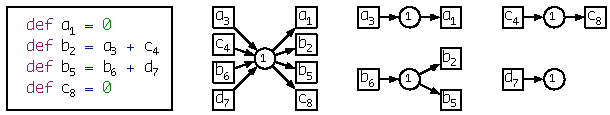
\includegraphics{figures/scope-graphs/global/example}
  \caption{%
    Program with variable declarations and references~(left), 
    corresponding scope graph~(center), and resolution graphs~(right).}
  \figurelabel{global}
\end{center}
\end{figure}

Depending on their syntactical position,
  instances have different roles in name binding.
A \emph{binding instance} introduces a new binding for the identifier in a certain scope.
In scope graphs, a directed edge \inlinegraphics{figures/scope-graphs/legend/definition} 
  connects a scope \inlinegraphics{figures/scope-graphs/legend/scope} 
  with a binding instance \inlinegraphics{figures/scope-graphs/legend/identifier} of that scope.
A \emph{referring instance} refers to a, potentially non-existing, binding instance of the same name in a certain scope.
If such a binding instance exists, the referring instance is a \emph{bound instance},
  otherwise it is a \emph{free instance}.
In scope graphs, a directed edge \inlinegraphics{figures/scope-graphs/legend/reference} 
  connects a referring instance \inlinegraphics{figures/scope-graphs/legend/identifier} 
  to its scope \inlinegraphics{figures/scope-graphs/legend/scope}.
In the example from \Figure{global},   
  all instances occur in the global scope \inlinegraphics{figures/scope-graphs/global/scopes} of the program
  which has incoming edges from referring instances \inlinegraphics{figures/scope-graphs/global/referring}
  and outgoing edges to its binding instances \inlinegraphics{figures/scope-graphs/global/binding}.
  
% \paragraph{Local resolution}
% 
% With scope graphs, name resolution corresponds to 
%   finding \emph{resolution paths} from referring instances to binding instances of the same name.
% In the scope graph from \Figure{global},
%   we cannot find a resolution path for \inlinegraphics{figures/scope-graphs/global/referring-c}.
% Thus, this instance is a free instance. 
% In contrast, 
%   we can find resolution paths to resolve 
%   \inlinegraphics{figures/scope-graphs/global/referring-a} and
%   \inlinegraphics{figures/scope-graphs/global/referring-b}, 
%   which makes those instances bound instances.
% So far, we only consider local resolution paths.



\newtheorem{definition}{Definition}
\begin{definition}[Local resolution path]
  A \emph{local resolution path for \smcode{i}} is
  a path \inlinegraphics{figures/scope-graphs/legend/local-resolution}
  from a referring instance %\inlinegraphics{figures/scope-graphs/legend/identifier} 
  to a binding instance %\inlinegraphics{figures/scope-graphs/legend/identifier} 
  of the same identifier \smcode{i}
  in the same scope \smcode{s}.
\end{definition}

%\paragraph{Local ambiguities}
%\paragraph{Local ambiguities.}

We can construct the \emph{resolution graph} of a particular instance,
  by restricting a scope graph to the nodes and edges from resolution paths of that instance.
\Figure{global} shows the resolution graphs for \inlinegraphics{figures/scope-graphs/global/referring-a} and
  \inlinegraphics{figures/scope-graphs/global/referring-b}.
Since their is only a single resolution path for \inlinegraphics{figures/scope-graphs/global/referring-a},
  its resolution graph is linear.
In contrast, the resolution graph for \inlinegraphics{figures/scope-graphs/global/referring-b} branches,
  since we can find paths to different binding instances \inlinegraphics{figures/scope-graphs/global/binding-b}.
We call such resolutions \emph{ambigous}.
In this case, the ambiguity is caused by 
  two conflicting binding instances \inlinegraphics{figures/scope-graphs/global/binding-b}
  in the same scope.
With scope graphs, we can define such conflicts in terms of paths:

\begin{definition}[Local conflict]
A binding instance \inlinegraphics{figures/scope-graphs/legend/definition} 
  \emph{conflicts locally}
  with another binding instance \inlinegraphics{figures/scope-graphs/legend/definition} 
  of the same identifier \smcode{i}
  in the same scope \smcode{s}.
\end{definition}

\paragraph{Lexical scoping}

A program typically defines several scopes.
For example, 
  the \kw{fix} and \kw{fun} expressions in the program in \Figure{lexical} 
  introduce two scopes for their argument expressions.
The corresponding scope graph in \Figure{lexical}
  represents these scopes as circle nodes 
    \inlinegraphics{figures/scope-graphs/lexical/fix-scope}
    \inlinegraphics{figures/scope-graphs/lexical/fun-scope}.
Scopes can be nested.
In scope graphs, a directed edge \inlinegraphics{figures/scope-graphs/legend/lexical} 
  connects a nested scope \inlinegraphics{figures/scope-graphs/legend/nested} 
  to its surrounding parent scope \inlinegraphics{figures/scope-graphs/legend/parent}.

\begin{figure}[htb]
\begin{center}
  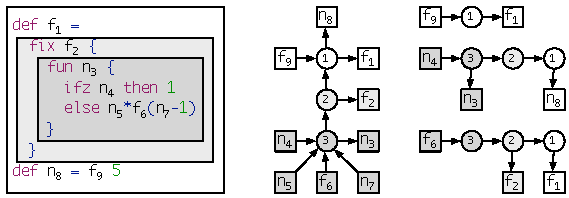
\includegraphics[trim=0.175cm 0cm 0cm 0cm]{figures/scope-graphs/lexical/example}
  \caption{%
    Lexical scopes in a function declaration~(left), 
    corresponding scope graph~(center), and resolution graphs~(right).}
  \figurelabel{lexical}
\end{center}
\end{figure}

In the example from \Figure{lexical},
  three scopes form a linear nesting hierarchy \inlinegraphics{figures/scope-graphs/lexical/nested}.
The two top-level variable declarations introduce two binding instances 
  \inlinegraphics{figures/scope-graphs/lexical/binding-f0}
  \inlinegraphics{figures/scope-graphs/lexical/binding-n0}
and a referring instance 
  \inlinegraphics{figures/scope-graphs/lexical/referring-f0}
in global scope \inlinegraphics{figures/scope-graphs/lexical/global-scope}.
The \kw{fix} expression introduces another binding instance 
  \inlinegraphics{figures/scope-graphs/lexical/binding-f1}
  in a new scope \inlinegraphics{figures/scope-graphs/lexical/fix-scope}
  which is nested in the global scope \inlinegraphics{figures/scope-graphs/lexical/global-scope}.
Finally, the \kw{fun} expression introduces another binding instance
  \inlinegraphics{figures/scope-graphs/lexical/binding-n2}
  and four referring instances 
  \inlinegraphics{figures/scope-graphs/lexical/referring-n2}
  \inlinegraphics{figures/scope-graphs/lexical/referring-f2}
  in a new scope \inlinegraphics{figures/scope-graphs/lexical/fun-scope}
  which is nested in the scope \inlinegraphics{figures/scope-graphs/lexical/fix-scope} of the fix expression.
 

%\paragraph{Lexical resolution}

A referring instance can be resolved either in its local scope or
  in one of its surrounding parent scopes.
Thus, we need to extend Definition~1 to allow chains of nested scopes.

\begin{definition}[Lexical resolution path]
A \emph{lexical resolution path for \smcode{i}} is
  a path \inlinegraphics{figures/scope-graphs/legend/lexical-resolution}
  from a referring instance 
  to a binding instance  
  of the same identifier \smcode{i}, 
    iff \inlinegraphics{figures/scope-graphs/legend/lexical-path} is a \emph{lexical scope path}.
Thereby, a \emph{lexical scope path} is either
a (degenerated) path \inlinegraphics{figures/scope-graphs/legend/scope}, or 
a path \inlinegraphics{figures/scope-graphs/legend/lexical-induct}
  from a nested scope \inlinegraphics{figures/scope-graphs/legend/nested-induct}
  to its ancestor scope \inlinegraphics{figures/scope-graphs/legend/parent}, 
    iff \inlinegraphics{figures/scope-graphs/legend/lexical-path} is a lexical scope path.
\end{definition}

\Figure{lexical} provides the resolution graphs according to the scope graph from the same figure.
First, \inlinegraphics{figures/scope-graphs/lexical/referring-f0} can be resolved locally.
Second, \inlinegraphics{figures/scope-graphs/lexical/referring-n2} can be resolved 
  either locally to \inlinegraphics{figures/scope-graphs/lexical/binding-n2} 
  or to \inlinegraphics{figures/scope-graphs/lexical/binding-n0} in the outermost surrounding scope.
Finally, \inlinegraphics{figures/scope-graphs/lexical/referring-f2} cannot be resolved locally but to
  \inlinegraphics{figures/scope-graphs/lexical/binding-f1} and
  \inlinegraphics{figures/scope-graphs/lexical/binding-f0} in its two surrounding scopes.


%\paragraph{Lexical ambiguities}

Hierarchies of nested lexical scopes introduce another source for ambiguous resolutions.
A referring instance can not only be resolved to conflicting binding instances in the same scope,
but also to conflicting binding instances in different scopes in the scope hierarchy.
Both ambiguities in the example from \Figure{lexical} are caused by the latter.
In the case of \inlinegraphics{figures/scope-graphs/lexical/referring-n2},
  the local binding instance \inlinegraphics{figures/scope-graphs/lexical/binding-n2}
  conflicts with \inlinegraphics{figures/scope-graphs/lexical/binding-n0}
  from the global scope.
In the case of \inlinegraphics{figures/scope-graphs/lexical/referring-f2},
  no local binding instance is involved.
  Instead, the conflict arises in the parent scope,
  where
    \inlinegraphics{figures/scope-graphs/lexical/binding-f1}
    conflicts with \inlinegraphics{figures/scope-graphs/lexical/binding-f0}
    from the global scope.

Such conflicts are typically resolved in favour of binding instances
  in scopes closer to the referring instances.
Binding instances in a nested scope \emph{shadow} 
  binding instances of the same name from surrounding scopes.
Similar to local conflicts, we can define shadowing in terms of paths in a scope graph.

\begin{definition}[Lexical shadowing]
A binding instance \inlinegraphics{figures/scope-graphs/legend/shadowing}
  \emph{shadows} 
  another binding instance \inlinegraphics{figures/scope-graphs/legend/shadowed} 
    of the same identifier \smcode{i}
  \emph{in scope \smcode{sn}},
  iff there exist a lexical scope path \inlinegraphics{figures/scope-graphs/legend/lexical-path}.
\end{definition}

With shadowing, name resolution corresponds to 
  finding paths from referring instances to unshadowed binding instances of the same name.
The ambiguities in the example from \Figure{lexical} are
  resolved in favour of the more local binding instances 
    \inlinegraphics{figures/scope-graphs/lexical/binding-n2} and
    \inlinegraphics{figures/scope-graphs/lexical/binding-f1}.

\paragraph{Alternative lexical scope hierarchies}

Similar syntactic structures can introduce different lexical scope hierarchies.
For example, 
  the programs in \Figure{let} employ different kinds of \kw{let} expressions,
    resulting in different scoping hierarchies for syntactically equivalent binding parts.
The \kw{letpar} expression introduces only a single scope \inlinegraphics{figures/scope-graphs/lets/body-scope} 
  for the body of the expression.
Binding instances \inlinegraphics{figures/scope-graphs/lets/par-bind} 
  from the binding parts are connected to the new scope.
As a consequence, referring instances \inlinegraphics{figures/scope-graphs/lets/par-bind-refer} 
  from the binding parts resolve to binding instances \inlinegraphics{figures/scope-graphs/lets/global-bind} 
  in the global scope.

\begin{figure}[htb]
\begin{center}
  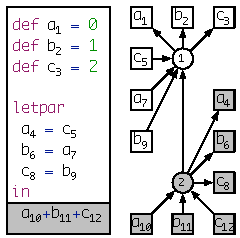
\includegraphics[trim=0.7cm 0cm 0cm 0cm]{figures/scope-graphs/lets/par}
  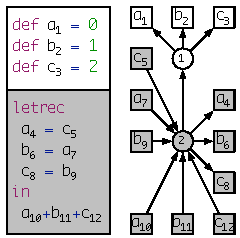
\includegraphics[trim=0.7cm 0cm 0cm 0cm]{figures/scope-graphs/lets/rec}
  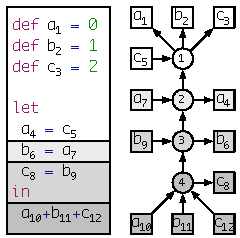
\includegraphics{figures/scope-graphs/lets/seq}
  \caption{Different kinds of let expressions and corresponding lexical scope hierarchies.}
  \figurelabel{let}
\end{center}
\end{figure}

The \kw{letrec} expression also introduces a single scope \inlinegraphics{figures/scope-graphs/lets/body-scope},
  but includes the binding parts in this scope.
This way, referring instances \inlinegraphics{figures/scope-graphs/lets/rec-bind-refer}
  from the binding parts now resolve to binding instances \inlinegraphics{figures/scope-graphs/lets/par-bind}
  from the binding parts.
Together with a disambiguation strategy which prefers local bindings, 
  binding parts can shadow other bindings in the whole \kw{letrec} expression.
Finally, the sequential \kw{let} expression introduces nested scopes \inlinegraphics{figures/scope-graphs/lets/scopes} 
  for each binding part.
These scopes include subsequent binding parts and the body of the \kw{let} expression.
In contrast to \kw{letrec} expressions,
  the same \kw{let} expression can bind instances of the same identifier multiple times,
  where new bindings shadow previous bindings.
Though, binding parts in \kw{let} expressions can only shadow bindings in subsequent binding parts and in the body,
  while binding parts in \kw{letrec} expressions can shadow bindings in preceding binding parts as well.
Hence, \inlinegraphics{figures/scope-graphs/lets/c2} resolves to \inlinegraphics{figures/scope-graphs/lets/c1}
  in global scope and not to \inlinegraphics{figures/scope-graphs/lets/c3} in a subsequent binding part.
  

% \begin{figure}[htb]
% \begin{center}
%   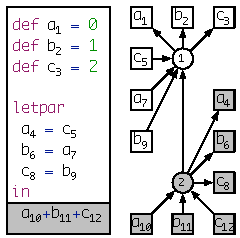
\includegraphics[trim=0.7cm 0cm 0cm 0cm]{figures/scope-graphs/lets/par}
%   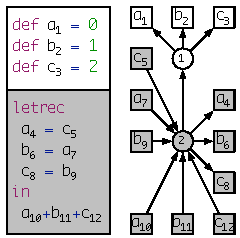
\includegraphics[trim=0.7cm 0cm 0cm 0cm]{figures/scope-graphs/lets/rec}
%   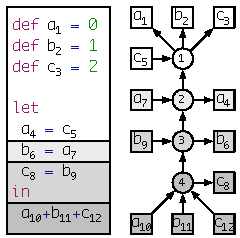
\includegraphics{figures/scope-graphs/lets/seq}
%   \caption{Scoping in different kinds of let expressions.}
%   \figurelabel{let}
% \end{center}
% \end{figure}

\paragraph{Named scopes and qualified names}

Language constructs might associate names with corresponding scopes.
For example, each module in the program in \Figure{qualified}
  associates a module name with the scope of the module, 
    which captures the declarations of the module.
We call such scopes \emph{named scopes}.
Binding instances in named scopes can be accessed from other scopes via the name of the scope.
For example, the program in \Figure{qualified} uses \emph{qualified names} to access declarations of a module from another module.

We introduce a second kind of edges, to model named scopes and qualified names.
A directed edge \inlinegraphics{figures/scope-graphs/legend/named} connects 
  a binding instance \inlinegraphics{figures/scope-graphs/legend/identifier} 
  to its associated named scope \inlinegraphics{figures/scope-graphs/legend/scope}.
A complementary directed edge \inlinegraphics{figures/scope-graphs/legend/qualified} connects 
  a qualified referring instance \inlinegraphics{figures/scope-graphs/legend/identifier} 
  to a qualifying referring instance \inlinegraphics{figures/scope-graphs/legend/qualifier}.
  
With qualified names, we can resolve to binding instances in a named scope, 
  even if these instances are not in the lexical scope of the referring instance.
In the example program in \Figure{qualified}, \inlinegraphics{figures/scope-graphs/qualified/b2} resolves to
  \inlinegraphics{figures/scope-graphs/qualified/b1}, which is not in the lexical scope of module \smcode{C}.
The corresponding resolution path includes the resolution path of the qualifier, 
  which is surrounded by two \inlinegraphics{figures/scope-graphs/legend/edge2} edges.
The opening edge  \inlinegraphics{figures/scope-graphs/qualified/opening} 
  is provided by the qualified name, 
  while the closing edge \inlinegraphics{figures/scope-graphs/qualified/closing} 
  is provided by a named scope.
The resolution path is completed by the binding instance \inlinegraphics{figures/scope-graphs/qualified/finish}.
%
The resolution of \inlinegraphics{figures/scope-graphs/qualified/b3} illustrates resolution of nested qualifiers.
In general, each nested qualifier needs to be resolved in the named scope of its preceeding qualifier, 
  before we can resolve the qualified name in the named scope of the last qualifier.
  
\begin{figure}[t]
\begin{center}
  %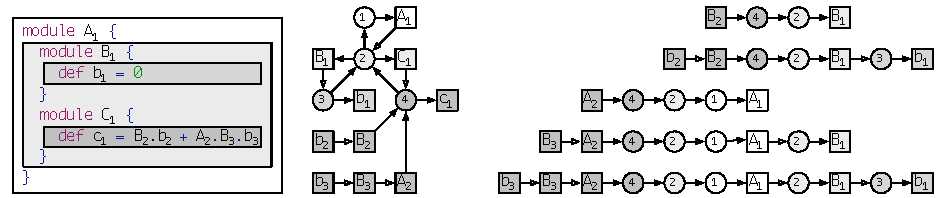
\includegraphics[trim=0.175cm 0cm 0cm 0cm]{figures/scope-graphs/qualified/example}
  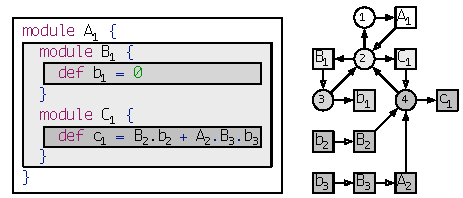
\includegraphics[trim=0.175cm 0cm 0cm 0cm]{figures/scope-graphs/qualified/example2}
  \vspace{0.35cm}
  
  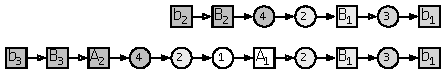
\includegraphics{figures/scope-graphs/qualified/resolution2}
  \caption{Named module scopes and qualified name access~(left), corresponding scope graph~(right) and resolution graphs~(bottom).}
  \figurelabel{qualified}
\end{center}
\end{figure}


\begin{definition}[Qualified resolution path]
  A path \inlinegraphics{figures/scope-graphs/legend/qualified-resolution}
  from a referring instance \inlinegraphics{figures/scope-graphs/legend/identifier} 
  to a binding instance \inlinegraphics{figures/scope-graphs/legend/identifier} of the same name
  is a \emph{qualified resolution path for \smcode{i}}, 
    iff \inlinegraphics{figures/scope-graphs/legend/qualifier-resolution} is 
      a lexical or qualified resolution path for \emph{\smcode{q}}.
\end{definition}

\paragraph{Imports}

Import directives introduce binding instances from a named scope into another scope.
In scope graphs, a directed edge \inlinegraphics{figures/scope-graphs/legend/import} connects 
  an importing scope \inlinegraphics{figures/scope-graphs/legend/scope}
  with a reference \inlinegraphics{figures/scope-graphs/legend/identifier} to the imported scope.
During resolution, these edges enable scope paths from importing scopes to imported scopes,
  making binding instances in the imported scope reachable for the importing scope.
This is orthogonal to lexical scoping, where scope paths from nested scopes to surrounding scopes
  make binding instances available to the nested scopes.  
Though, lexical scoping and importing cannot be combined arbitrarily.
While resolution should consider imports in surrounding scopes,
  it should not consider surrounding scopes of imported scopes.
This leads to the following definition of resolution paths:

\begin{definition}[Resolution path]
A \emph{resolution path for \smcode{i}} is either
  a path \inlinegraphics{figures/scope-graphs/legend/lexical-resolution}, 
    iff \inlinegraphics{figures/scope-graphs/legend/lexical-path} is a \emph{scope path}, or
  a path \inlinegraphics{figures/scope-graphs/legend/qualified-resolution},
    iff \inlinegraphics{figures/scope-graphs/legend/qualifier-resolution} is a resolution path for \emph{\smcode{q}}.

Thereby, a \emph{scope path} is either
  a (degenerated) path \inlinegraphics{figures/scope-graphs/legend/scope}, or 
  a path \inlinegraphics{figures/scope-graphs/legend/lexical-induct}, 
    iff \inlinegraphics{figures/scope-graphs/legend/lexical-path} is a scope path, or
  a path \inlinegraphics{figures/scope-graphs/legend/import-induct}, 
    iff \inlinegraphics{figures/scope-graphs/legend/lexical-path} is a scope path and
    \inlinegraphics{figures/scope-graphs/legend/import-resolution} is a resolution path for \emph{\smcode{j}}.
\end{definition}

\Figure{includes} shows an example program with three modules.
To resolve \inlinegraphics{figures/scope-graphs/imports/vb1} in \inlinegraphics{figures/scope-graphs/imports/s2},
  we need to consider the import of \inlinegraphics{figures/scope-graphs/imports/B1},
  which resolves to \inlinegraphics{figures/scope-graphs/imports/B2}.
In its associated scope \inlinegraphics{figures/scope-graphs/imports/s3},
  we find \inlinegraphics{figures/scope-graphs/imports/vb2} 
  and another import \inlinegraphics{figures/scope-graphs/imports/C1},
  which resolves to \inlinegraphics{figures/scope-graphs/imports/C2}.
In its associated scope \inlinegraphics{figures/scope-graphs/imports/s4}, 
  we find \inlinegraphics{figures/scope-graphs/imports/vb3}. 
%   
This ambigous resolution is caused by a conflict between 
  the local binding instance \inlinegraphics{figures/scope-graphs/imports/vb2}
  and the imported binding instance \inlinegraphics{figures/scope-graphs/imports/vb3}.
In general, a conflict occurs, 
if two local or imported binding instances have the same name.

\begin{definition}[Conflict]
A binding instance \inlinegraphics{figures/scope-graphs/legend/conflict1}
  \emph{conflicts in scope} \inlinegraphics{figures/scope-graphs/legend/scope}  with 
  another binding instance \inlinegraphics{figures/scope-graphs/legend/conflict2} of the same name,
  iff there exist local scope paths 
    \inlinegraphics{figures/scope-graphs/legend/conflict3} and
    \inlinegraphics{figures/scope-graphs/legend/conflict-4}.

\noindent Thereby, a \emph{local scope path} is either
  a (degenerated) path \inlinegraphics{figures/scope-graphs/legend/scope}, or 
  a path \inlinegraphics{figures/scope-graphs/legend/import-induct}, 
    iff \inlinegraphics{figures/scope-graphs/legend/lexical-path} is a local scope path and
    \inlinegraphics{figures/scope-graphs/legend/import-resolution} is a resolution path for \emph{\smcode{j}}.
\end{definition}

\begin{figure}[t]
\begin{center}
  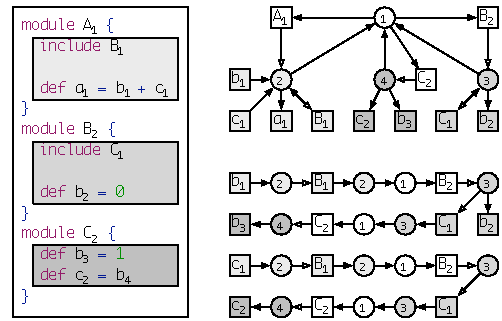
\includegraphics[trim=0.175cm 0cm 0cm 0cm]{figures/scope-graphs/imports/include}
  \caption{Includes of modules.}
  \figurelabel{includes}
  \bigskip
  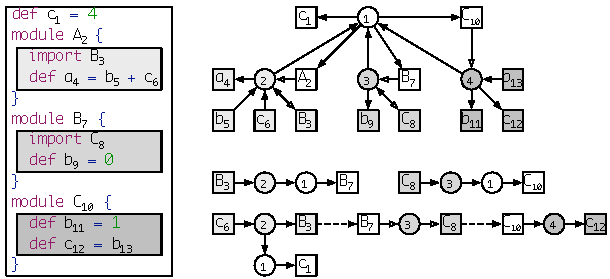
\includegraphics[trim=0.175cm 0cm 0cm 0cm]{figures/scope-graphs/imports/imports}
  \caption{Imports of modules.}
  \figurelabel{imports}
\end{center}
\end{figure}

\paragraph{Alternative import scope hierarchies}

Earlier in this section, we showed that similar syntactic constructs might yield different lexical scope hierarchies.
This also holds for import scope hierarchies.
For example, the program in \Figure{imports} is a variant of the previous program from \Figure{includes},
  where local declarations can hide imported declarations and local imports hide transitive imports.
Each module now introduces two nested scopes.
Import edges connect only to the outer scope.
This way, local declarations can hide imported declarations.
For example, 
  the resolution of \inlinegraphics{figures/scope-graphs/imports/vb1} in \Figure{imports} 
  does no longer has a conflict between a local declaration and an imported declaration.
Though, the resolution is still ambigous.
The ambiguity is caused by module names which are now associated with two scopes.
This is needed to still allow for transitive imports, 
  where both local declarations and imported declarations can be imported.
The ambiguity can be resolved by an explicit order of scopes associated with names.
In the case of \kw{import} directives, we want to prefer the inner scope of a module (for local definitions) 
  over its outer scope (for imports).

% \begin{definition}[Shadowing]
% A binding instance \inlinegraphics{figures/scope-graphs/legend/identifier}
%   \emph{shadows} another binding instance \inlinegraphics{figures/scope-graphs/legend/shadowed} of the same name
%   \emph{in scope \smcode{sn}},
%   iff there exist a local scope path \ldots 
%   and a scope path \inlinegraphics{figures/scope-graphs/legend/lexical-path}.
% \end{definition}

	\newpage\clearpage
	\section{A Theory of Visibility}

naming conflict: multiple resolution paths for same identifier

some naming conflicts are resolved by policies for visibility 

thesis: shadowing / visibility is independent / orthogonal to resolution paths

systematic analysis of the design space of shadowing as expressed in terms of path well-formedness and specificity ordering
\begin{itemize}
 \item  model different kinds of imports through flags on imports
\item transitive vs non-transitive vs non-transitive+export
\item include vs import vs prefer-imported: maybe use a precedence value in the imports
\item imports with inherited lexical scope (handled by well-formedness)
\end{itemize}

Add flags to imports to describe the different policies, should be handled by well-formedness of the resolution path

\newcommand{\flag}[1]{\overline{#1}}

\paragraph{Import Policies}
To reflect the different imports policies, we add boolean flags to the imports,
when no flag is specified the default behavior is used.
Assume some \emph{import B} is declared in a module {\it A},
\begin{itemize}
 \item If the Import/Export flag $e$ of this import is $0$ then the definition in {\it B} are visible in $A$ and if it is $1$ the definitions
  in {\it B} are also visible from every scope importing \emph{A}.
 \item If the transitivity flag $t$ is $0$ then the resolution can only use the definitions or exports of the imported module else
  the resolution can use all the import clauses in the imported scopes
 \item If the parent (recursive) flag $r$ is $0$ then the resolution process can only continue through possible imports else it 
  can also look into the parent scope
\end{itemize}
The flag of an import is thus a triple of booleans and denoted $\flag{etr}$, for example a non-transitive export that do not allow recursive call
to parent has flag $\flag{100}$.


% The precedence flag $pr^{F}$ can be either set to:
%   \begin{itemize}
%    \item Usual import $u$ whose precedence is lower than the definition, thus a resolution using directly a definition is preferred
%     over an usual import
%    \item Include import $i$ whose precedence is the same than a definition
%    \item Pref import $p$ whose precedence is higher than a definition, such an import is preferred over a direct definition
%   \end{itemize}

??? what if we want priority of import over parents ? for example import with same precedence as parent, parent preferred over imports ??? 
Back to the idea of giving a precedence to imports in algorithm: try to resolve with precedence n, if you find something then done else try with
prec (n+1), parent and definition are only one of these way.

Automata in Figure \ref{fig:algoterm} for the correctness of the path, the states corresponds to different authorization first component is the transitivity flag, i.e. are you allowed to 
use simple imports, second component is the parent flag, i.e. can you look inside the parent scope. Transitions are either parent rule $P$, or imports flags 

\begin{figure}
\centering
\begin{tikzpicture}[shorten >=1pt,auto]

\tikzset{>=stealth',
    every edge/.append style={->}
  }
      \node[circle,draw] (TR) at (0,2.6) {\it 11};
      \node[circle,draw] (TX) at (4.5,5.2) {\it 10};
      \node[circle,draw] (NX) at (3,2.6) {\it 00};
      \node[circle,draw] (NR) at (4.5,0) {\it 01};
      \node (ri) at (4.5,2) {};
      
     \path 

     (TR) edge[loop left] node[left] {\small $\flag{x11} + P$} (TR)
     (TR.90) edge[bend left=35] node[above left] {\small $\flag{x10}$} (TX.175)
     (TR) edge[bend left=10] node[above] {\small $\flag{x00}$} (NX)
     (TR.280) edge[bend right=35] node[above right] {\small $\flag{x01}$} (NR.175)

     (TX) edge[loop above] node[above] {\small $\flag{x10}$} (TX)
          edge[bend left=10] node[right] {\small $\flag{x00}$} (NX)
     (TX.185) edge[bend right=35] node[below right] {\small $\flag{x11}$} (TR.80)
     (TX.340) edge[bend left=50] node[right] {\small $\flag{x01}$} (NR.20)

     (NX) edge[loop right] node[right] {\small $\flag{100}$} (NX)
          edge[bend left=10] node[left] {\small $\flag{110}$} (TX)
          edge[bend left=10] node[right] {\small $\flag{101}$} (NR)
     (NX) edge[bend left=10]  node[below] {\small $\flag{111}$} (TR)

     (NR) edge[loop below] node[below] {\small $\flag{101} + P$} (NR)
     (NR.30) edge[bend right=50] node[left] {\small $\flag{110}$} (TX.330)
     (NR) edge[bend left=10] node[left] {\small $\flag{100}$} (NX)
     (NR.185) edge[bend left=35] node[below left] {\small $\flag{111}$} (TR.270);

\end{tikzpicture}
%\rule{\textwidth}{.1pt}
\caption{Path Well Formedness Automata}
\label{fig:algoterm}
\end{figure}


\begin{figure}
\begin{boxedminipage}{\hsize}

\textbf{Edges in scope graph}

\smallskip

	\infrule{R}{
		x^p \in \R{S}
	}{
		\mathcal{I} \vdash x^p \scopea{x}{R(x^p)} S
	}
	
\smallskip

	\infrule{D}{
		d_x \in \D{S}
	}{
		\mathcal{I} \vdash S \scopea{x}{D(d_x)} d_x
  }

\smallskip

% 	\infrule{T}{}{
% 		\mathcal{I} \vdash S_1\cdot S_2\cdot S^* \scopea{x}{T} S_2 \cdot S^*
% 	}

% \smallskip

	\infrule{Par}{
		\P{S} = S'
	}{
		\mathcal{I} \vdash S \scopea{x}{Par} S'
	}

\smallskip

	\infrule{I}{
		y^p \in \mathcal{I}(S_1)  
		\tab 
		y^p \notin \mathcal{I} 
		\tab
		y^p\!,\mathcal{I} \vdash y^p \resolvea{P^*}\!\!\!d_y^{S_2}		
	}{
		\mathcal{I} \vdash S_1 \scopea{x}{I^t(y^p,P^*)} S_2 
	}

\smallskip

% 	\infrule{I}{
% 		y^p \in \I{S_1}  
% 		\tab 
% 		y^p \notin \mathcal{I} 
% 		\tab
% 		y^p\!,\mathcal{I} \vdash y^p \resolvea{P^*}\!\!\!d_y^{S_2^*}	
% 	}{
% 		\mathcal{I} \vdash S_1\cdot S_1^* \scopea{x}{I(y^p\!,P^*)} S_2^* 
% 	}

% \smallskip

\textbf{Path composition}

	\infrule{C1}{}{
		\mathcal{I} \vdash d_x \lra{[]}{x} d_x
	}

\smallskip

	\infrule{C2}{
		\mathcal{I} \vdash A \scopea{x}{P} B
		\tab 
		\mathcal{I} \vdash B \lra{P^*}{x} C
	}{
		\mathcal{I} \vdash A \lra{P\cdot P^*}{x} C
	}

\smallskip
\textbf{Resolution}

	\infrule{Res}{
 		\begin{array}{c}
    	\mathcal{I} \vdash x^p \lra{P^*_1}{x} d_x
			\tab
			\tab
			\tab
			P^*_1 : WFP
    	\\
  		\forall d'_x,P^*_2(\mathcal{I} \vdash x^p \lra{P^*_2}{x} d'_x\Rightarrow\neg
  	P^*_2 < P^*_1)
  	\end{array}
	}{
		\mathcal{I} \vdash x^p \resolvea{P^*_1} d_x
	}

\bigskip


\end{boxedminipage}
\caption{Resolution Calculus}
\label{fig:calculus}
\end{figure}


%\begin{figure}[p]

\begin{minipage}[t]{.49\hsize}
\begin{boxedminipage}[t]{\hsize}
\textbf{References and declarations}
\begin{itemize}
  \item $\mbox{$\dsi{x}{i}{S}$}$: declaration with name $x$ at position $i$ and optional
  associated named scope $S$
  \item $\ri{x}{i}$: reference with name $x$ 
  at position~$i$ 
\end{itemize}
\textbf{Scope graph}
\begin{itemize}
  \item $\G$: scope graph
  \item $\S{\G}$: scopes $S$ in $\G$ 
  \item $\D{S}$: declarations $\dsi{x}{i}{S'}$ in $S$
  \item $\R{S}$: references $\ri{x}{i}$ in $S$
  \item $\I{S}$: imports $\ri{x}{i}$ in $S$
  \item $\P{S}$: parent scope of $S$
\end{itemize}
\textbf{Well-formedness properties}
\begin{itemize}
  \item $\P{S}$ is a partial function
  \item The parent relation is well-founded
  \item Each $\ri{x}{i}$ and $\di{x}{i}$ appears in exactly one scope $S$
\end{itemize}
\end{boxedminipage}
\caption{Scope graphs}
\figurelabel{scope-graph}
\end{minipage}
\begin{minipage}[t]{.49\hsize}
\begin{boxedminipage}[t]{\hsize}
\textbf{Resolution paths}
\vspace*{-0.4\baselineskip}
$$\begin{array}{rl}
          s & := \dstep{\di{x}{i}}\ |\ \istep{\ri{x}{i}}{\dsi{x}{j}{S}}\ |\ \pstep\\
          p & := []\ |\ s\ |\ p\cdot p\\
          & \mbox{\rm (inductively generated)} \\[0pt]
          [] \cdot p & = p \cdot [] = p\\
          (p_1 \cdot p_2) &\cdot\ p_3  = p_1 \cdot (p_2 \cdot p_3)
\end{array}$$ 

\textbf{Well-formed paths}

\vspace*{-0.5\baselineskip}

\[
	   \WF(p) \Leftrightarrow p \in \pstep^* \cdot \istep{\_}{\_}^* 
\]
	
\textbf{Specificity ordering on paths}

%\bigskip

	\infrule{DI}{}{
		\dstep{\_} < \istep{\_}{\_}
	}

\medskip

	\infrule{IP}{}{
		\istep{\_}{\_} < \pstep 
	}

\medskip

	\infrule{DP}{}{
		 \dstep{\_} < \pstep
	}

\medskip

    \infrule{Lex1}{
		s_1 < s_2
	}{ 
		s_1\cdot p_1 < s_2 \cdot p_2
	}


\medskip

	\infrule{Lex2}{
		p_1 < p_2
	}{ 
		s \cdot p_1 < s \cdot p_2
	}

\smallskip

\end{boxedminipage}
\caption{Resolution paths, well-formedness predicate, and specificity
ordering.}
\figurelabel{order}
\end{minipage}

\bigskip

\begin{boxedminipage}{\hsize}
\textbf{Edges in scope graph}
\smallskip

	\infrule{P}{
		\P{S_1} = S_2
	}{
		\seeni \vdash \pstep : S_1 \edge S_2
	}

\medskip

	\infrule{I}{
		\ri{y}{i} \in \I{S_1}\setminus\seeni  
		\tab
		\seeni \vdash p : \ri{y}{i} \resolve \dsi{y}{j}{S_2}
	}{
		\seeni \vdash \istep{\ri{y}{i}}{\dsi{y}{j}{S_2}} : S_1 \edge S_2 
	}

\medskip
\textbf{Transitive closure}

%\medskip
       
	\infrule{N}{
		}{
		\seeni \vdash [] : A \medge A
	}

\medskip

	\infrule{T}{
		\seeni \vdash s : A \edge B
		\tab 
		\seeni \vdash p : B \medge C
	}{
		\seeni \vdash s \cdot p : A \medge C
	}

\smallskip

\textbf{Reachable declarations}
\medskip

	\infrule{R}{
		\di{x}{i} \in \D{S'}
		\tab
		\seeni \vdash p : S \medge S'
		\tab 
		\WF(p)
	}{
		\seeni \vdash p \cdot \dstep{\di{x}{i}} : S \reach \di{x}{i}
	}

\medskip

\textbf{Visible declarations}
\medskip

\infrule{V}{
 	\seeni \vdash p : S \reach \di{x}{i}
			\tab
			\tab
			% tab
  		\forall j,p' (
  		   \seeni \vdash p' : S \reach \di{x}{j} \Rightarrow 
  		   \neg (p' < p)
  		)
  	}{
		\seeni \vdash {p} : S \resolve \di{x}{i}
	}

\medskip

\textbf{Reference resolution}

\medskip 

\infrule{X}{
		\ri{x}{i} \in \R{S}
    \tab
    \{ \ri{x}{i} \} \cup \seeni \vdash p : S \resolve \di{x}{j}
	}{
		\seeni \vdash p : \ri{x}{i} \resolve \di{x}{j}
	}
\end{boxedminipage}
\caption{Resolution calculus}
\figurelabel{rescalc}



\end{figure}




Set of \emph{seen-imports} : 
\begin{itemize}
 \item how do we introduce it ?
 \item in which cases is it really necessary ?
\end{itemize}

%%% Local Variables: 
%%% mode: latex
%%% TeX-master: "../document"
%%% End: 

	\newpage\clearpage
	\section{Resolution Automata}

the calculus depends on recursive invocations

derive a (non-deterministic) resolution automaton from the calculus

$S1 \rightarrow_x S2 \rightarrow_x S3 \rightarrow_x S4$

$S1 \rightarrow [x] S2 \rightarrow [y,x] S2 \rightarrow [y,x] S3 \rightarrow [x] S4$

formalize calculus

prove correspondence to the first calculus

- produces same paths
- apply same well-formedness \& specificity ordering

	\newpage\clearpage
	\section{Evaluation}\label{evaluation}

\begin{itemize}
\itemsep1pt\parskip0pt\parsep0pt
\item
  Coverage: can we express the name binding patterns of real languages?
\end{itemize}




%%% Local Variables: 
%%% mode: latex
%%% TeX-master: t
%%% End: 
